\section{Validation against Hu et al.\ (2017) and Smith et al.\ (2021)}
\label{sec:validation}

\subsection{Setup}

\code{examples/SubgridTests/StromgrenSphereClumpSmith2021/} reproduces
both papers' D-type expansion test directly: four co-located
19.2\,M$_\odot$ sources ($\dot N_{\rm ion}\approx2.5\times10^{48}\,
{\rm s^{-1}}$ each, $1\times10^{49}\,{\rm s^{-1}}$ combined), a uniform
$100\,{\rm cm^{-3}}$, $10^3\,$K background, and a 10\,pc-radius,
$10^4\,{\rm cm^{-3}}$ clump 20\,pc from the sources -- all confirmed
against the papers' own text, not assumed. Both papers report the
initial (equilibrium, no clump) Str\"omgren radius as 3.1\,pc for this
configuration, and reach $\sim$20--25\,pc by $t=8\,$Myr in the
uniform-medium, no-clump case; Smith et al.'s Fig.~2 (with the clump
present) shows their spherical scheme partially disrupting the clump
by 8\,Myr, and their HealPix scheme leaving it largely intact while the
front elsewhere reaches close to the no-clump reference. This is the
comparison every run below reproduces at two gas resolutions:
\code{gas\_mass=20} (matching \citeauthor{Smith2021}'s own resolution
for this test) and \code{gas\_mass=95} (a representative galaxy
zoom-in baryon particle mass).

\subsection{Why every run below uses $Z/Z_\odot\approx0.231$}
\label{sec:metallicity}

Both reference papers are effectively zero-metallicity (\citet{Hu2017}
state their D-type test medium is ``composed of pure hydrogen'';
neither paper's recombination rate or temperature floor has a
metallicity term at all) and clamp ionized gas to a flat $10^4\,$K.
This code's own temperature floor (Eq.~\ref{eq:floor}) is
metallicity-\emph{dependent}: at $Z=0$ the applied temperature is
$\approx$47,500\,K, not $10^4\,$K, which raises $r_{\rm HII}$ through
two independent channels -- a lower case-B recombination coefficient
(Section~\ref{sec:beta-temperature}) and a higher D-type driving sound
speed ($c_s\propto\sqrt T$) -- so a $Z=0$ run is expected to overshoot
the papers' reference, and can run large enough to hit
\code{Stars:max\_HII\_search\_radius} (45\,pc) or the box half-width
(50\,pc).

Both channels are neutralized by construction at the metallicity where
$T_{\rm collisional}=10^4\,$K exactly (Eq.~\ref{eq:tcollisional}):
\begin{equation}
  \frac{0.86}{1+0.22\log_{10}(Z/Z_\odot)} = 1
  \quad\Longrightarrow\quad Z/Z_\odot \approx 0.231.
  \label{eq:z0231}
\end{equation}
Every validation run below uses this metallicity
(\code{initial\_metallicity=0.231}). This gives a direct,
apples-to-apples comparison against the papers' own convention --
without needing to widen the box or search radius, since the front no
longer overshoots enough to approach either default ceiling.

\subsection{The $Z/Z_\odot\approx0.231$ matrix at \texttt{gas\_mass=20}}
\label{sec:matrix-gas20}

This is the direct replacement for Smith et al.'s Fig.~2 comparison
(spherical vs.\ HealPix), at \citeauthor{Smith2021}'s own gas
resolution, run at the metallicity that removes the two systematic
channels from Section~\ref{sec:metallicity} so the comparison is a fair
one.

\begin{center}
\begin{tabular}{lrrr}
  \hline
  scheme  & rebuild=0.01\,Myr & rebuild=0.05\,Myr & rebuild=0.1\,Myr \\
  \hline
  uniform (nside=0) & 12.5--14.3\,pc & 12.5--13.2\,pc & 13.3--13.6\,pc \\
  angular (nside=1) & 24.7--27.7\,pc & 13.2--20.5\,pc & 12.2--14.0\,pc \\
  \hline
\end{tabular}
\end{center}

\textbf{The uniform scheme is consistently low, regardless of rebuild
cadence} (12.5--14.3\,pc across all three) -- the clump's mass-biasing
(Section~\ref{sec:angular-splitting}) suppresses it the same way at
this finer resolution as at \code{gas\_mass=95}
(Section~\ref{sec:matrix-gas95}); this is a scheme limitation, not a
resolution effect.

\textbf{The angular scheme only matches the papers at the fast rebuild
cadence.} At \code{rebuild=0.01\,Myr} (this example's default) it
reaches 24.7--27.7\,pc, right in the papers' $\sim$20--25\,pc range,
and Figure~\ref{fig:gas20-slices} shows this is a genuine match, not a
bookkeeping artifact: $r_{\rm physics}=21.05\,$pc for the star shown,
close to $r_{\rm HII}=27.72\,$pc, with a visibly intact, symmetric
bubble showing the clump's expected notch on its near side -- closely
matching \citeauthor{Smith2021}'s HealPix panel. At
\code{rebuild=0.05\,Myr} the result degrades and scatters
(13.2--20.5\,pc, only one of four stars reaching the reference band),
and at \code{rebuild=0.1\,Myr} it collapses to the same
$\approx$13\,pc as the uniform scheme -- \emph{the angular scheme's
entire benefit over uniform disappears at slow rebuild cadences.} This
makes physical sense: each of the 12 angular pixels holds only
$\dot N_{\rm ion}/12$ of the budget: at a slow cadence a pixel that
exhausts its small share early has nothing left to spend until the next
rebuild, which is exactly the starvation the fast cadence avoids. A
second, not-yet-tested candidate contributor: at $Z/Z_\odot\approx0.231$
metal-line cooling is far more efficient than at $Z=0$ (unlike the
tagged/floored interior, gas that has aged out of its tag but not yet
been re-tagged cools on its own, per item e7,
Section~\ref{sec:open}), so a slow rebuild cadence may let more of the
front cool back below the tagging threshold between rebuilds at this
metallicity than it would at $Z=0$ -- consistent with the fast cadence
mattering more here than it appeared to in the earlier $Z=0$ sweep.
Not isolated from the pixel-starvation effect above; both point the
same direction.
\textbf{Conclusion: \code{rebuild=0.01\,Myr} is not just the papers'
own convention -- at this resolution, it is necessary for the angular
scheme to do what it is meant to do.} This is a stronger justification
for this example's existing default than was available before this
matrix.

\begin{figure}
  \centering
  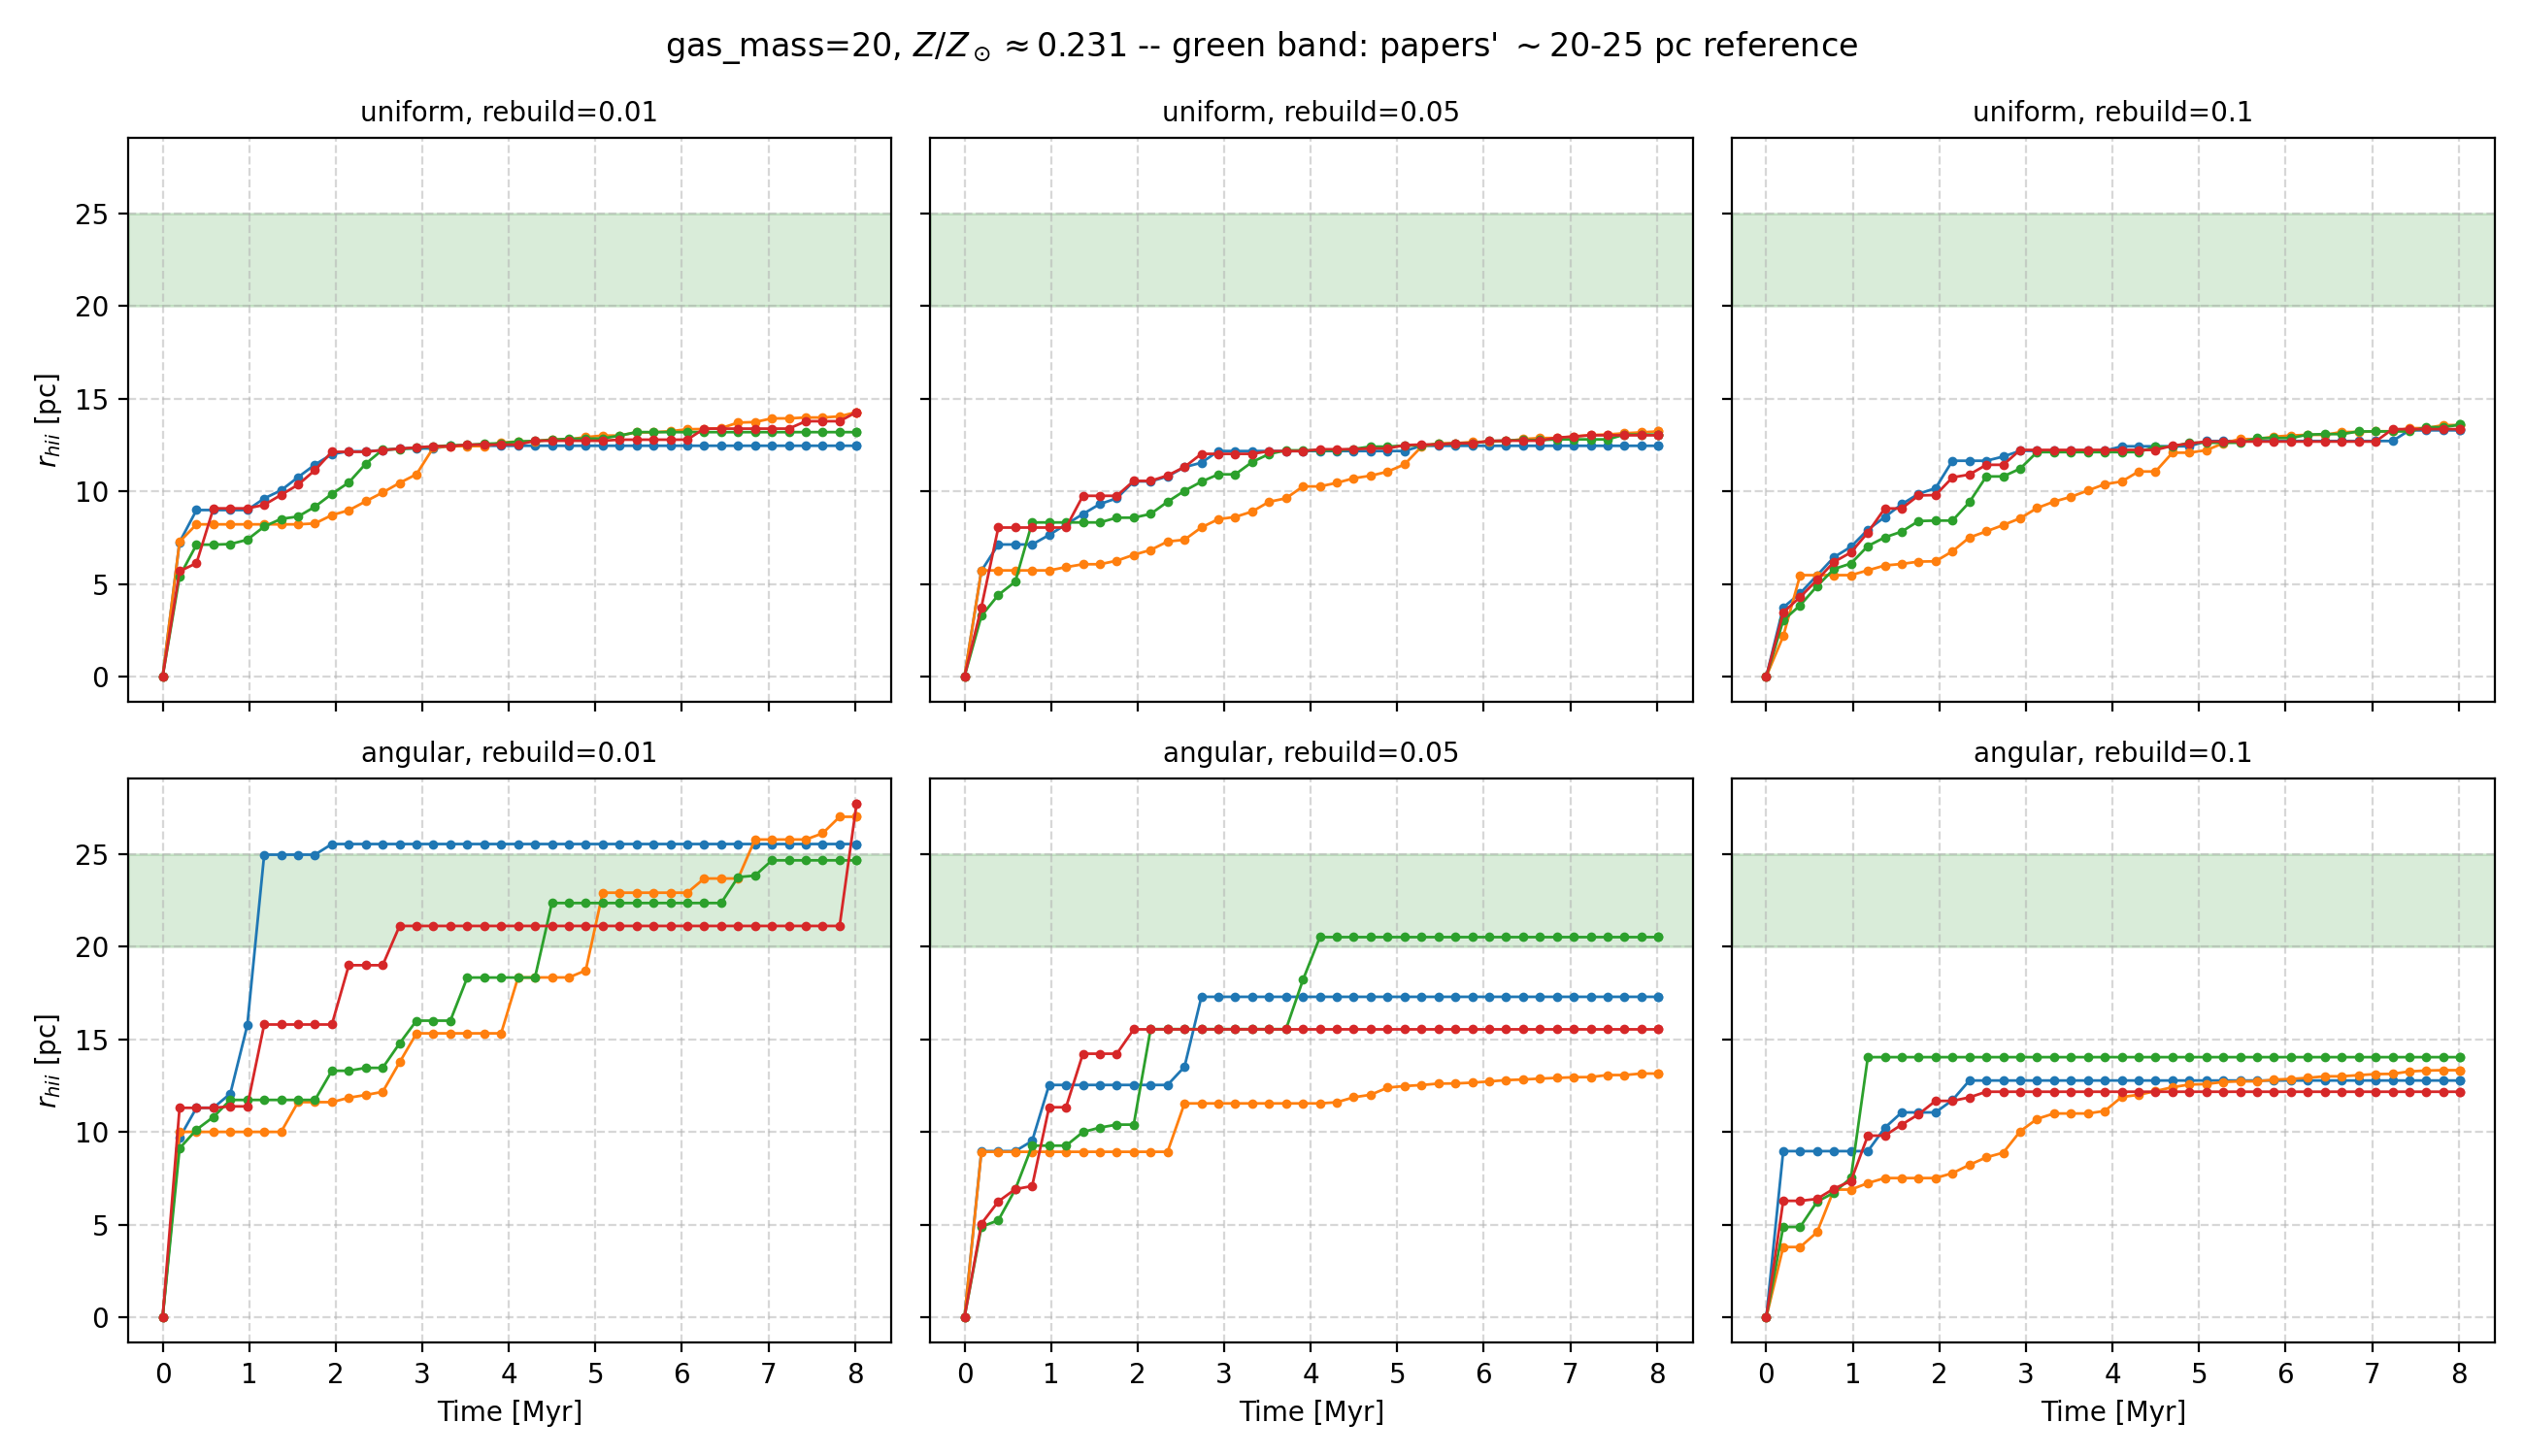
\includegraphics[width=\linewidth]{Figures/gas20_z0231_matrix}
  \caption{Per-star $r_{\rm HII}(t)$ at \texttt{gas\_mass=20},
    $Z/Z_\odot\approx0.231$, for all six configurations. Green band:
    the papers' $\sim$20--25\,pc reference. Only the angular,
    fast-rebuild case (bottom left) consistently reaches it.}
  \label{fig:gas20-growth}
\end{figure}

\begin{figure}
  \centering
  \begin{tabular}{@{}c@{}c@{}c@{}}
    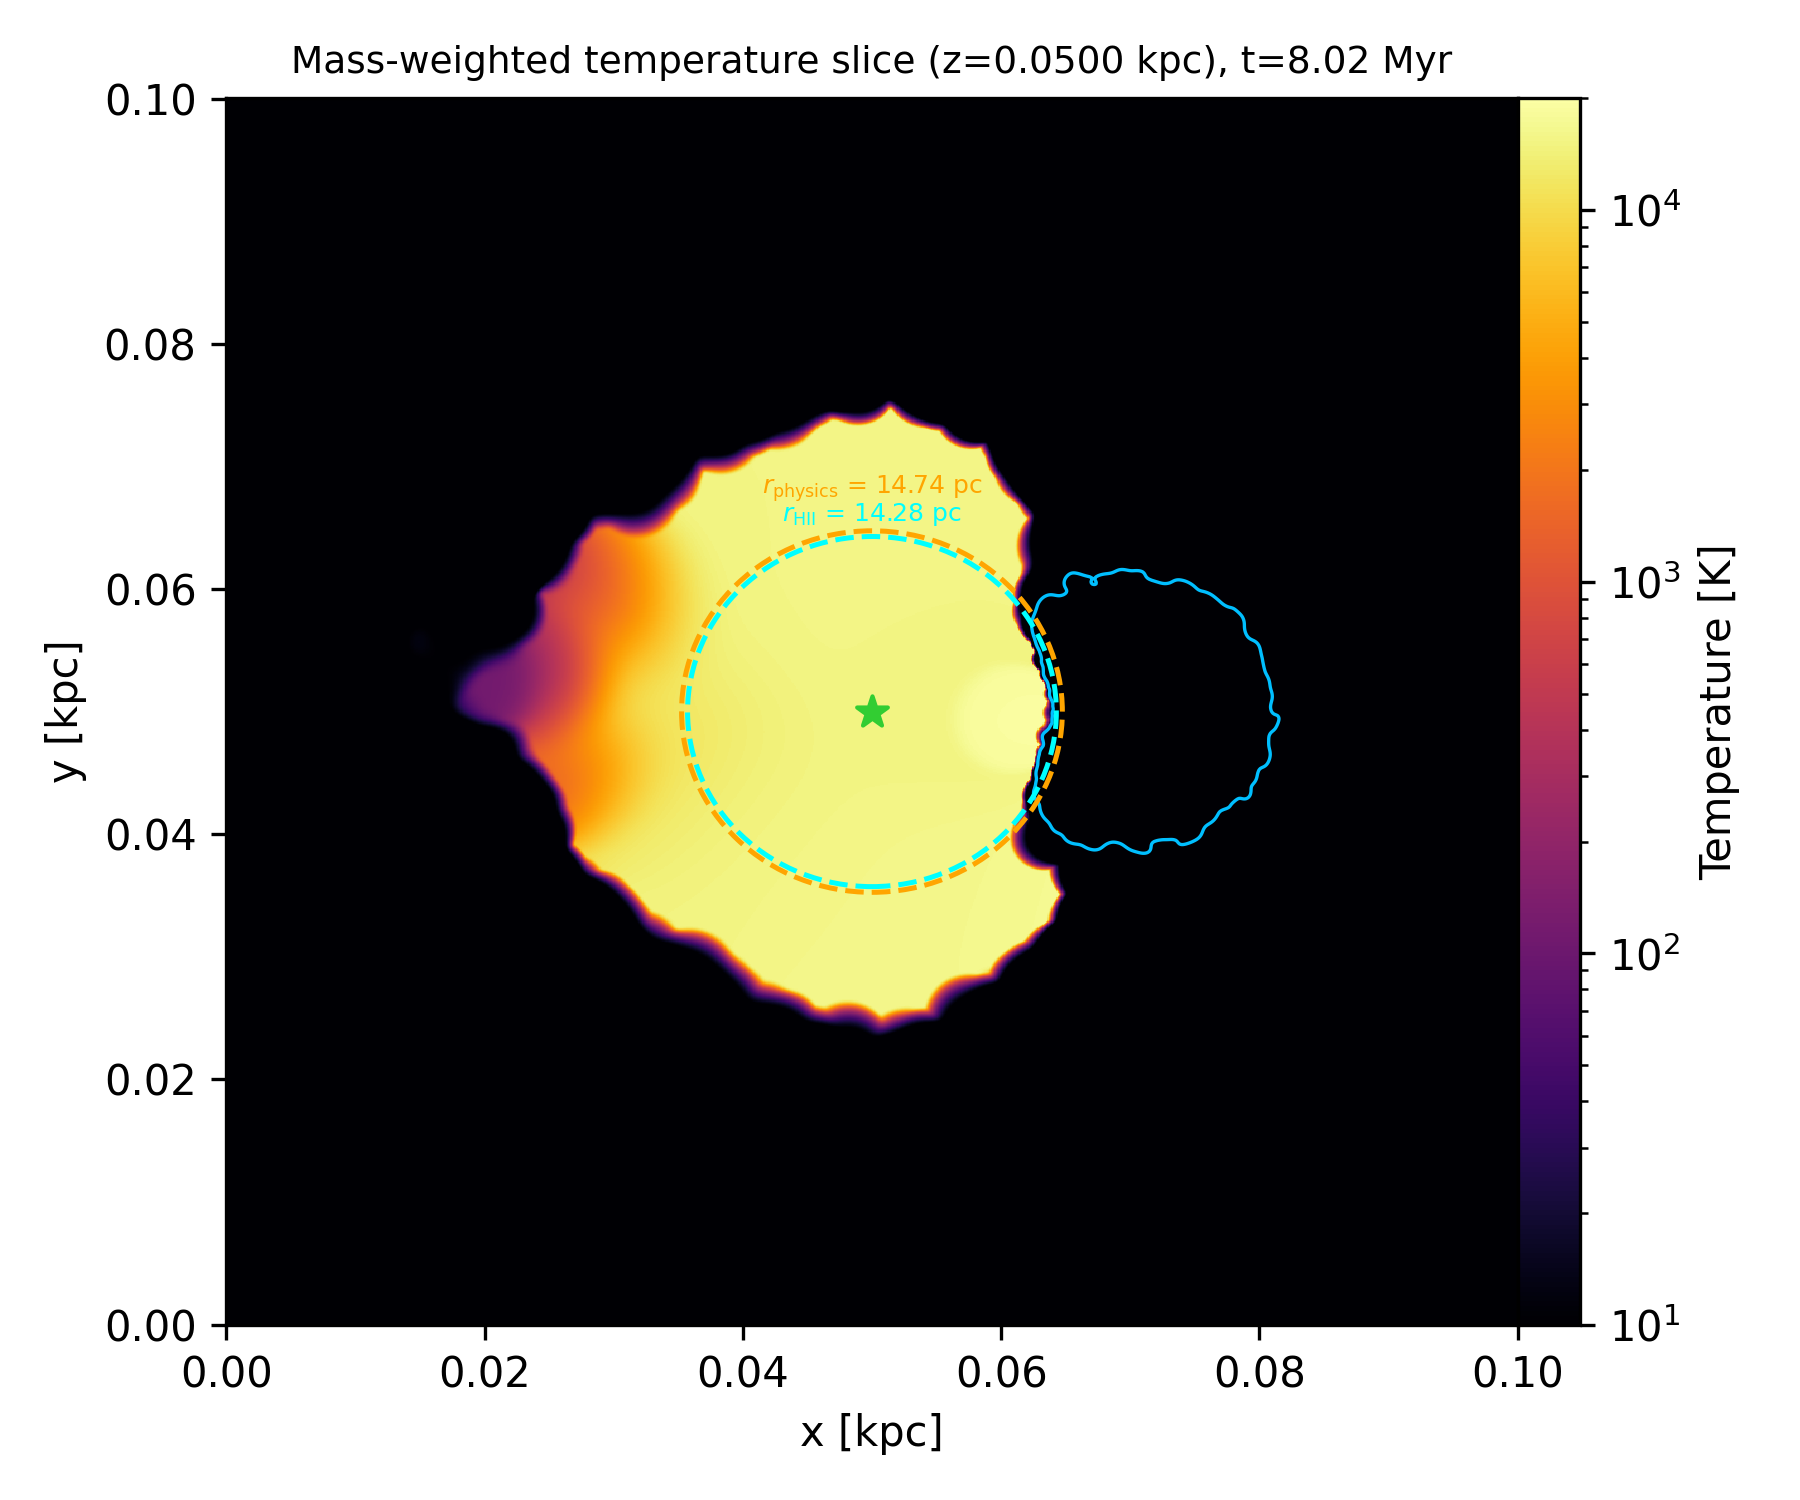
\includegraphics[width=0.325\linewidth]{Figures/tslice_gas20_nside0_rebuild0p01} &
    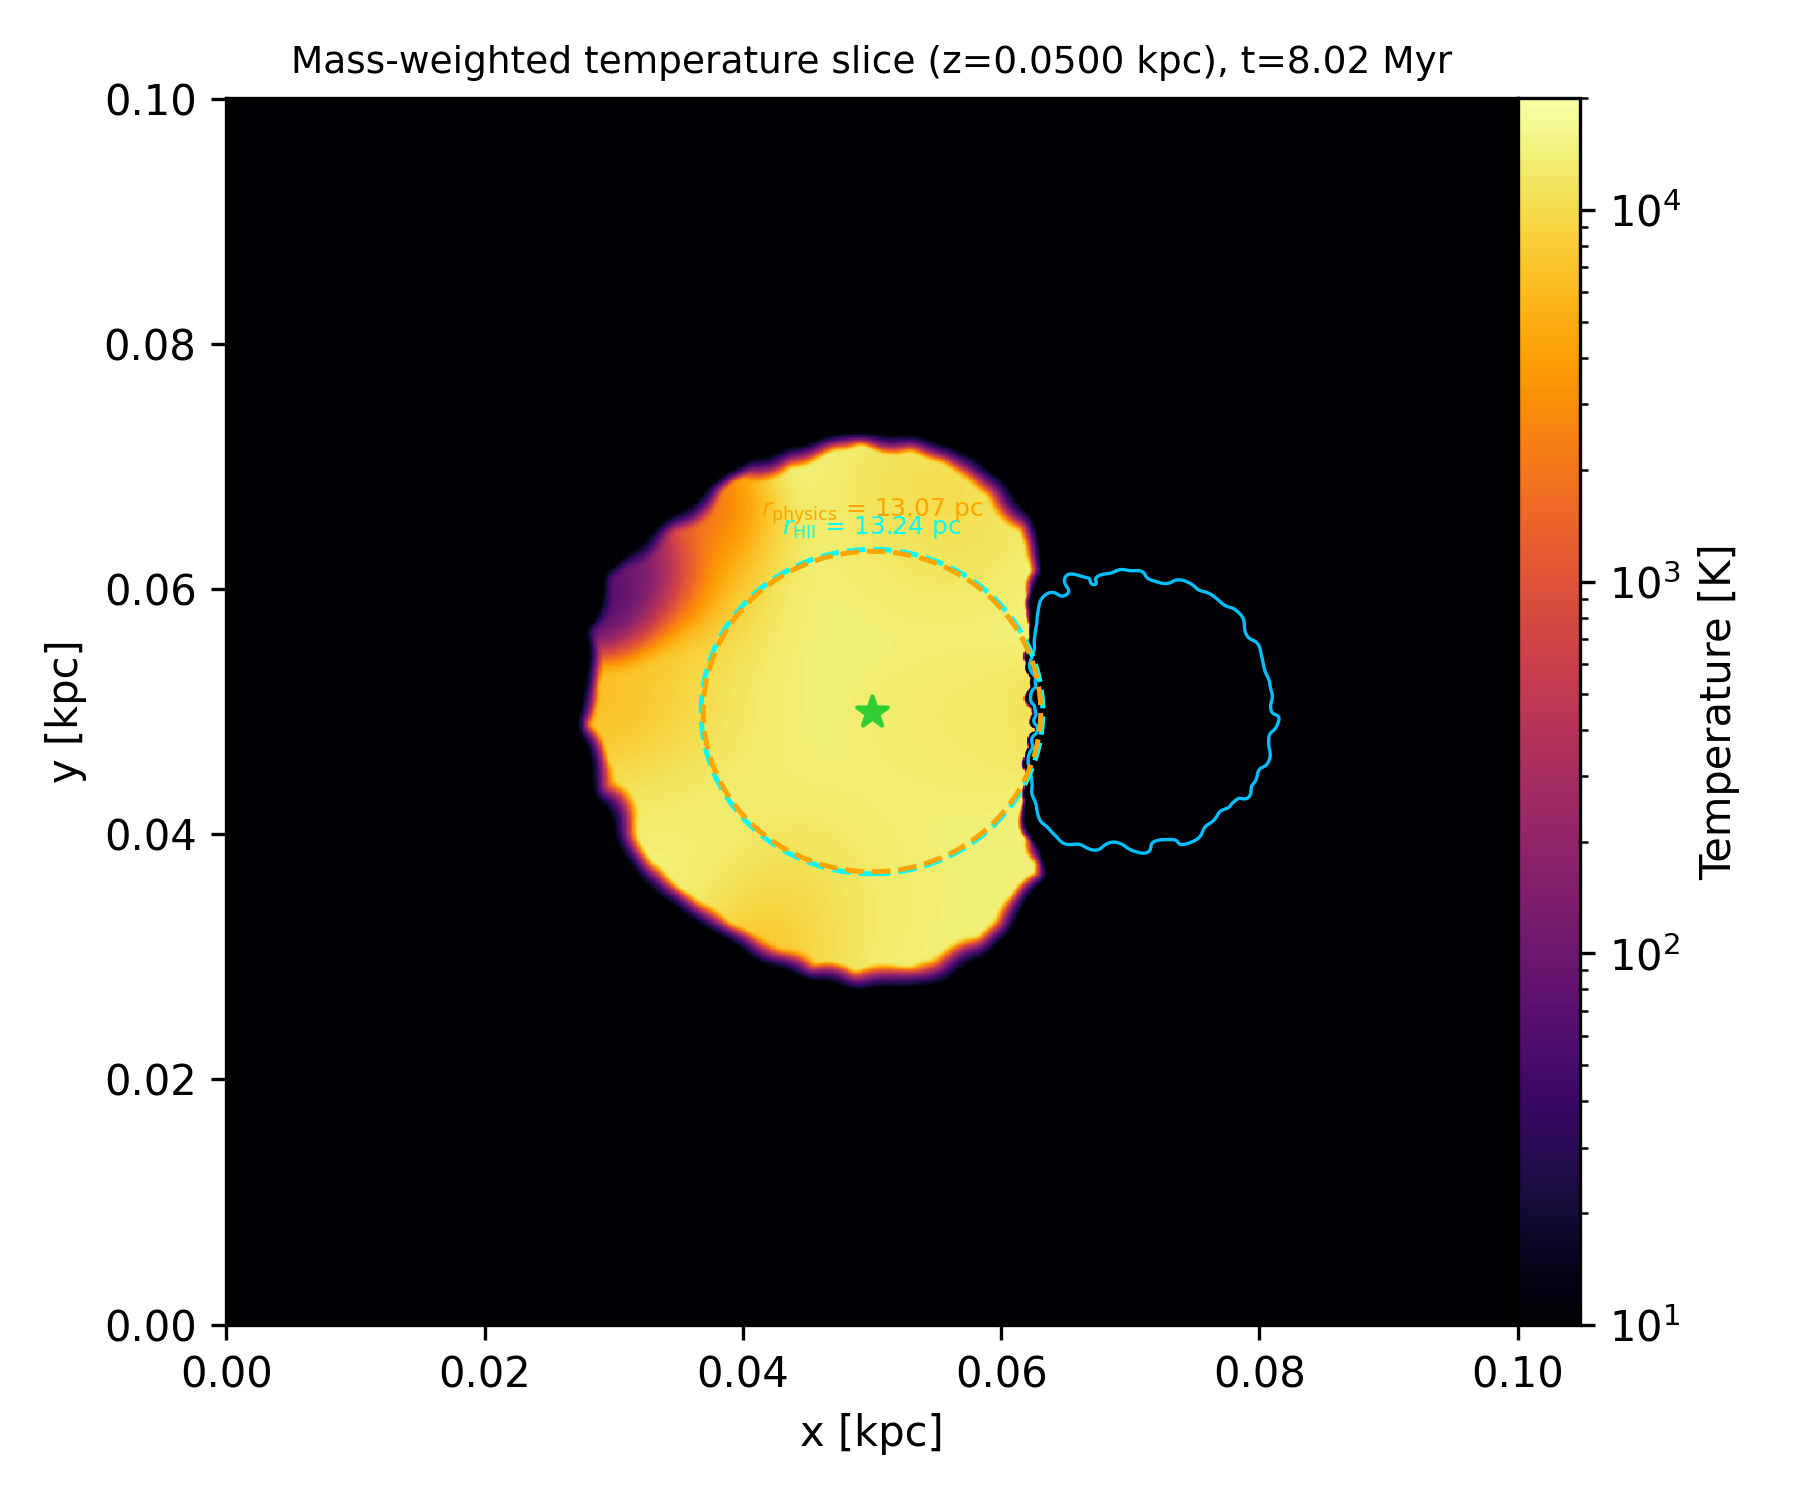
\includegraphics[width=0.325\linewidth]{Figures/tslice_gas20_nside0_rebuild0p05} &
    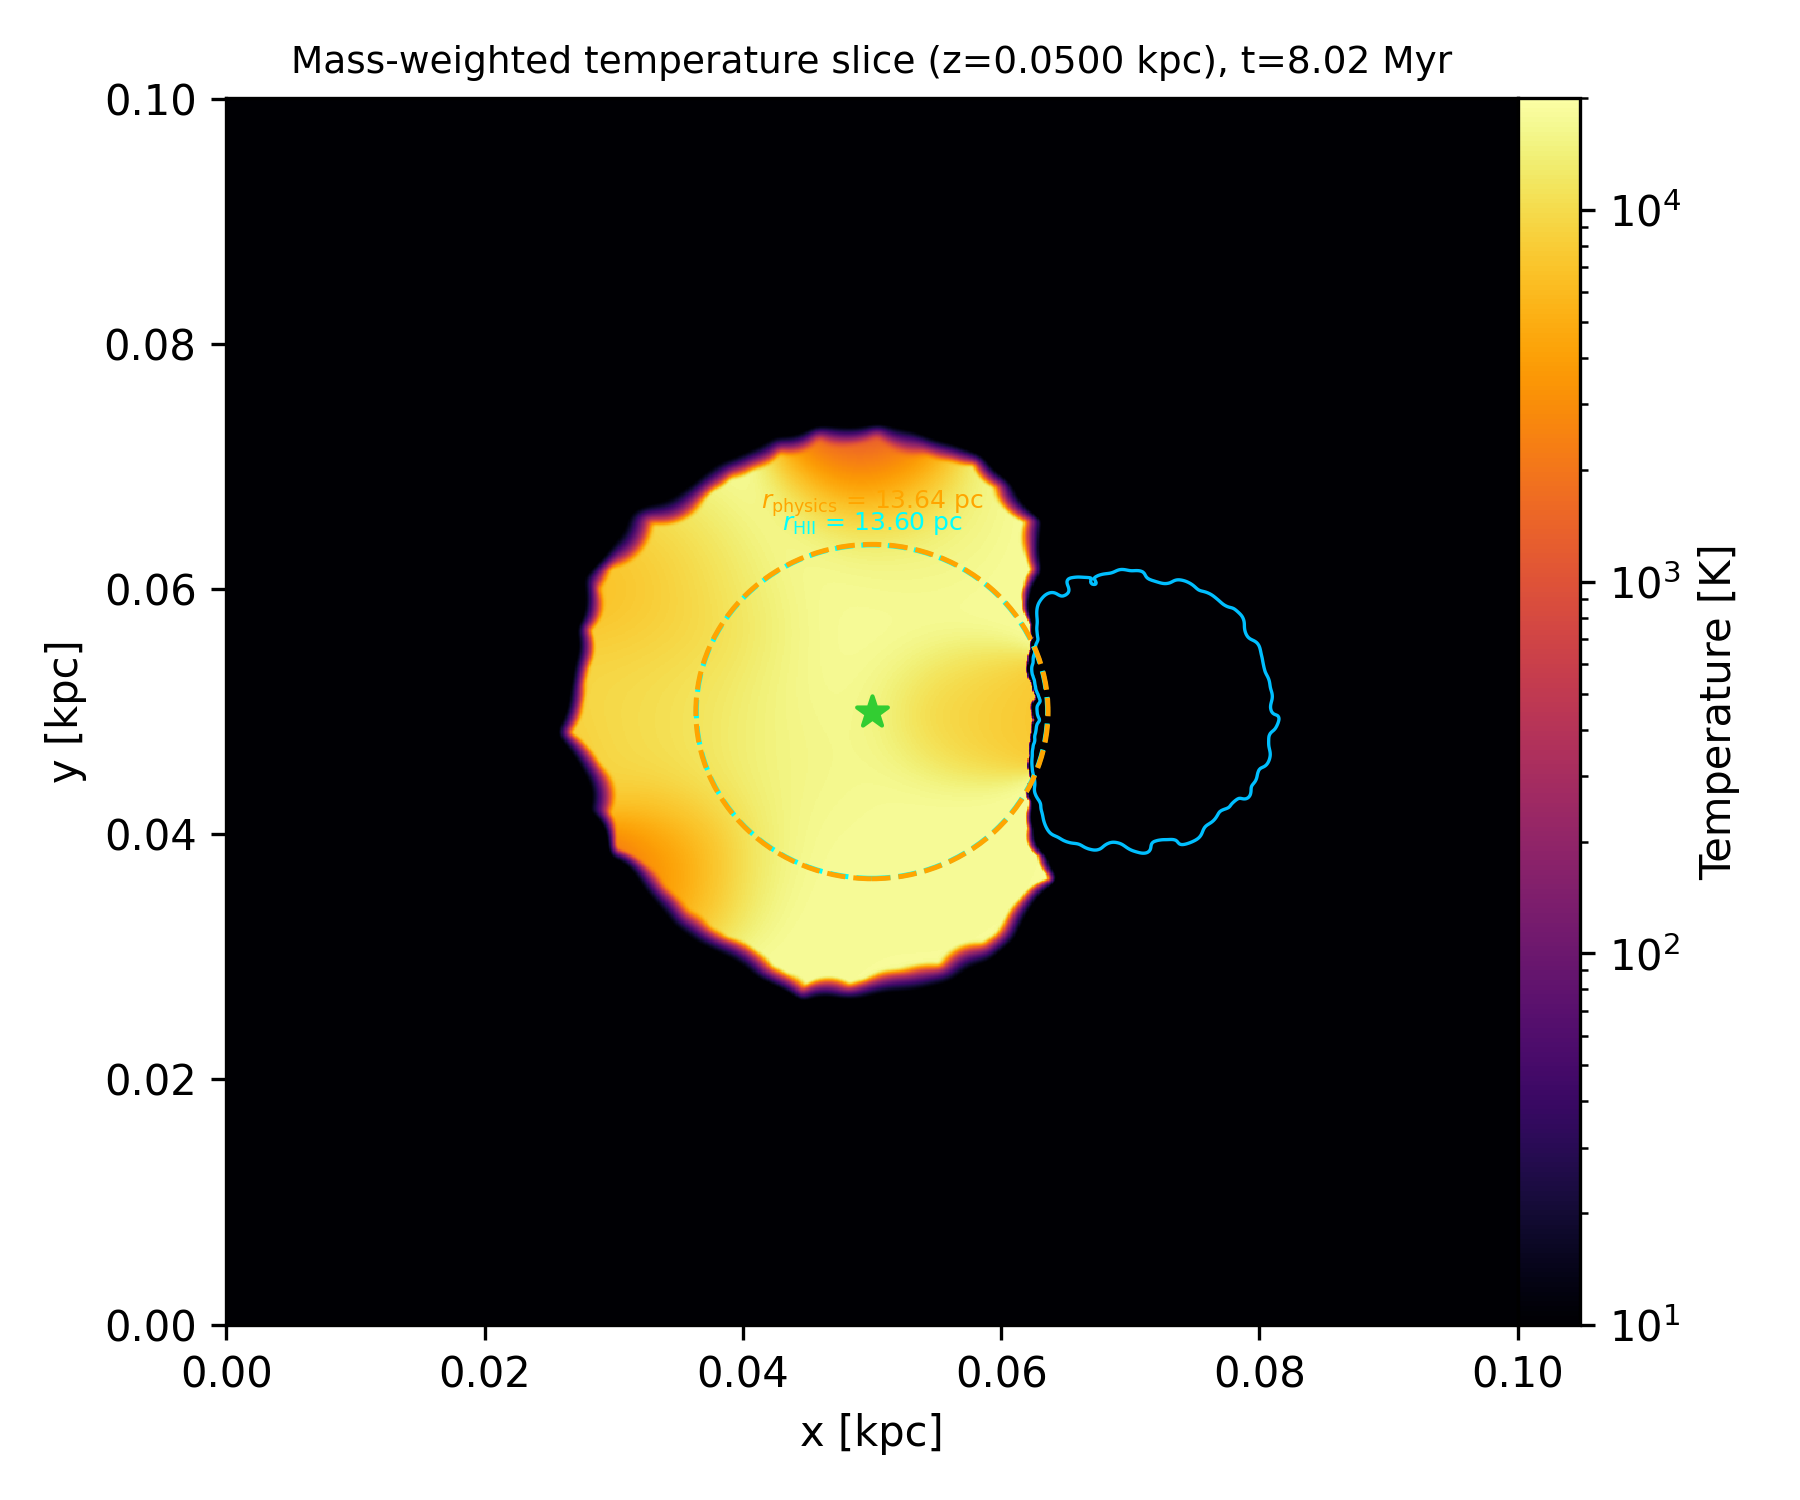
\includegraphics[width=0.325\linewidth]{Figures/tslice_gas20_nside0_rebuild0p1} \\
    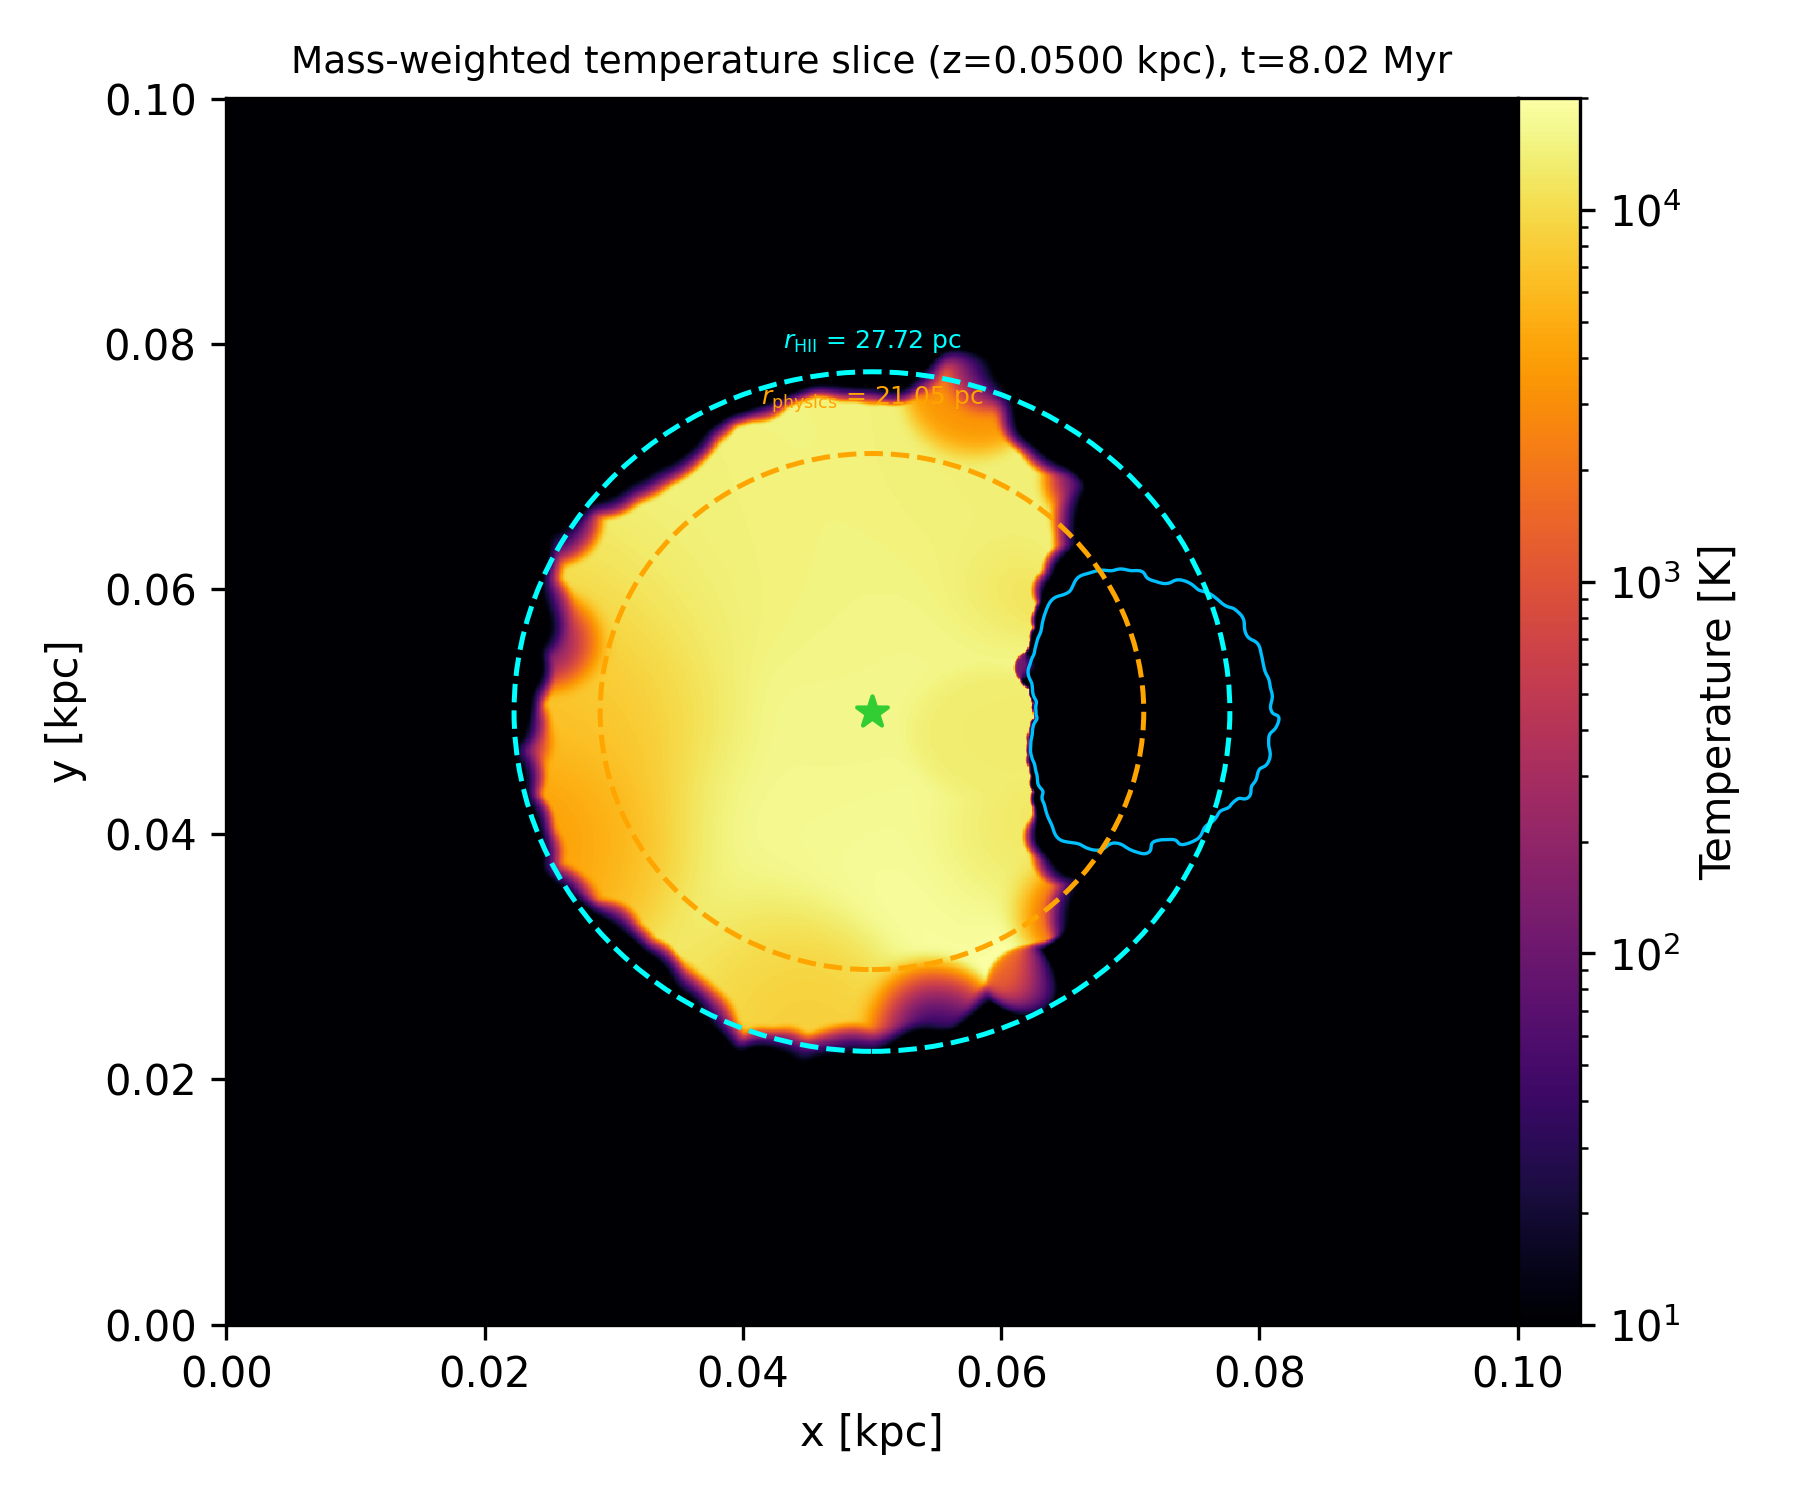
\includegraphics[width=0.325\linewidth]{Figures/tslice_gas20_nside1_rebuild0p01} &
    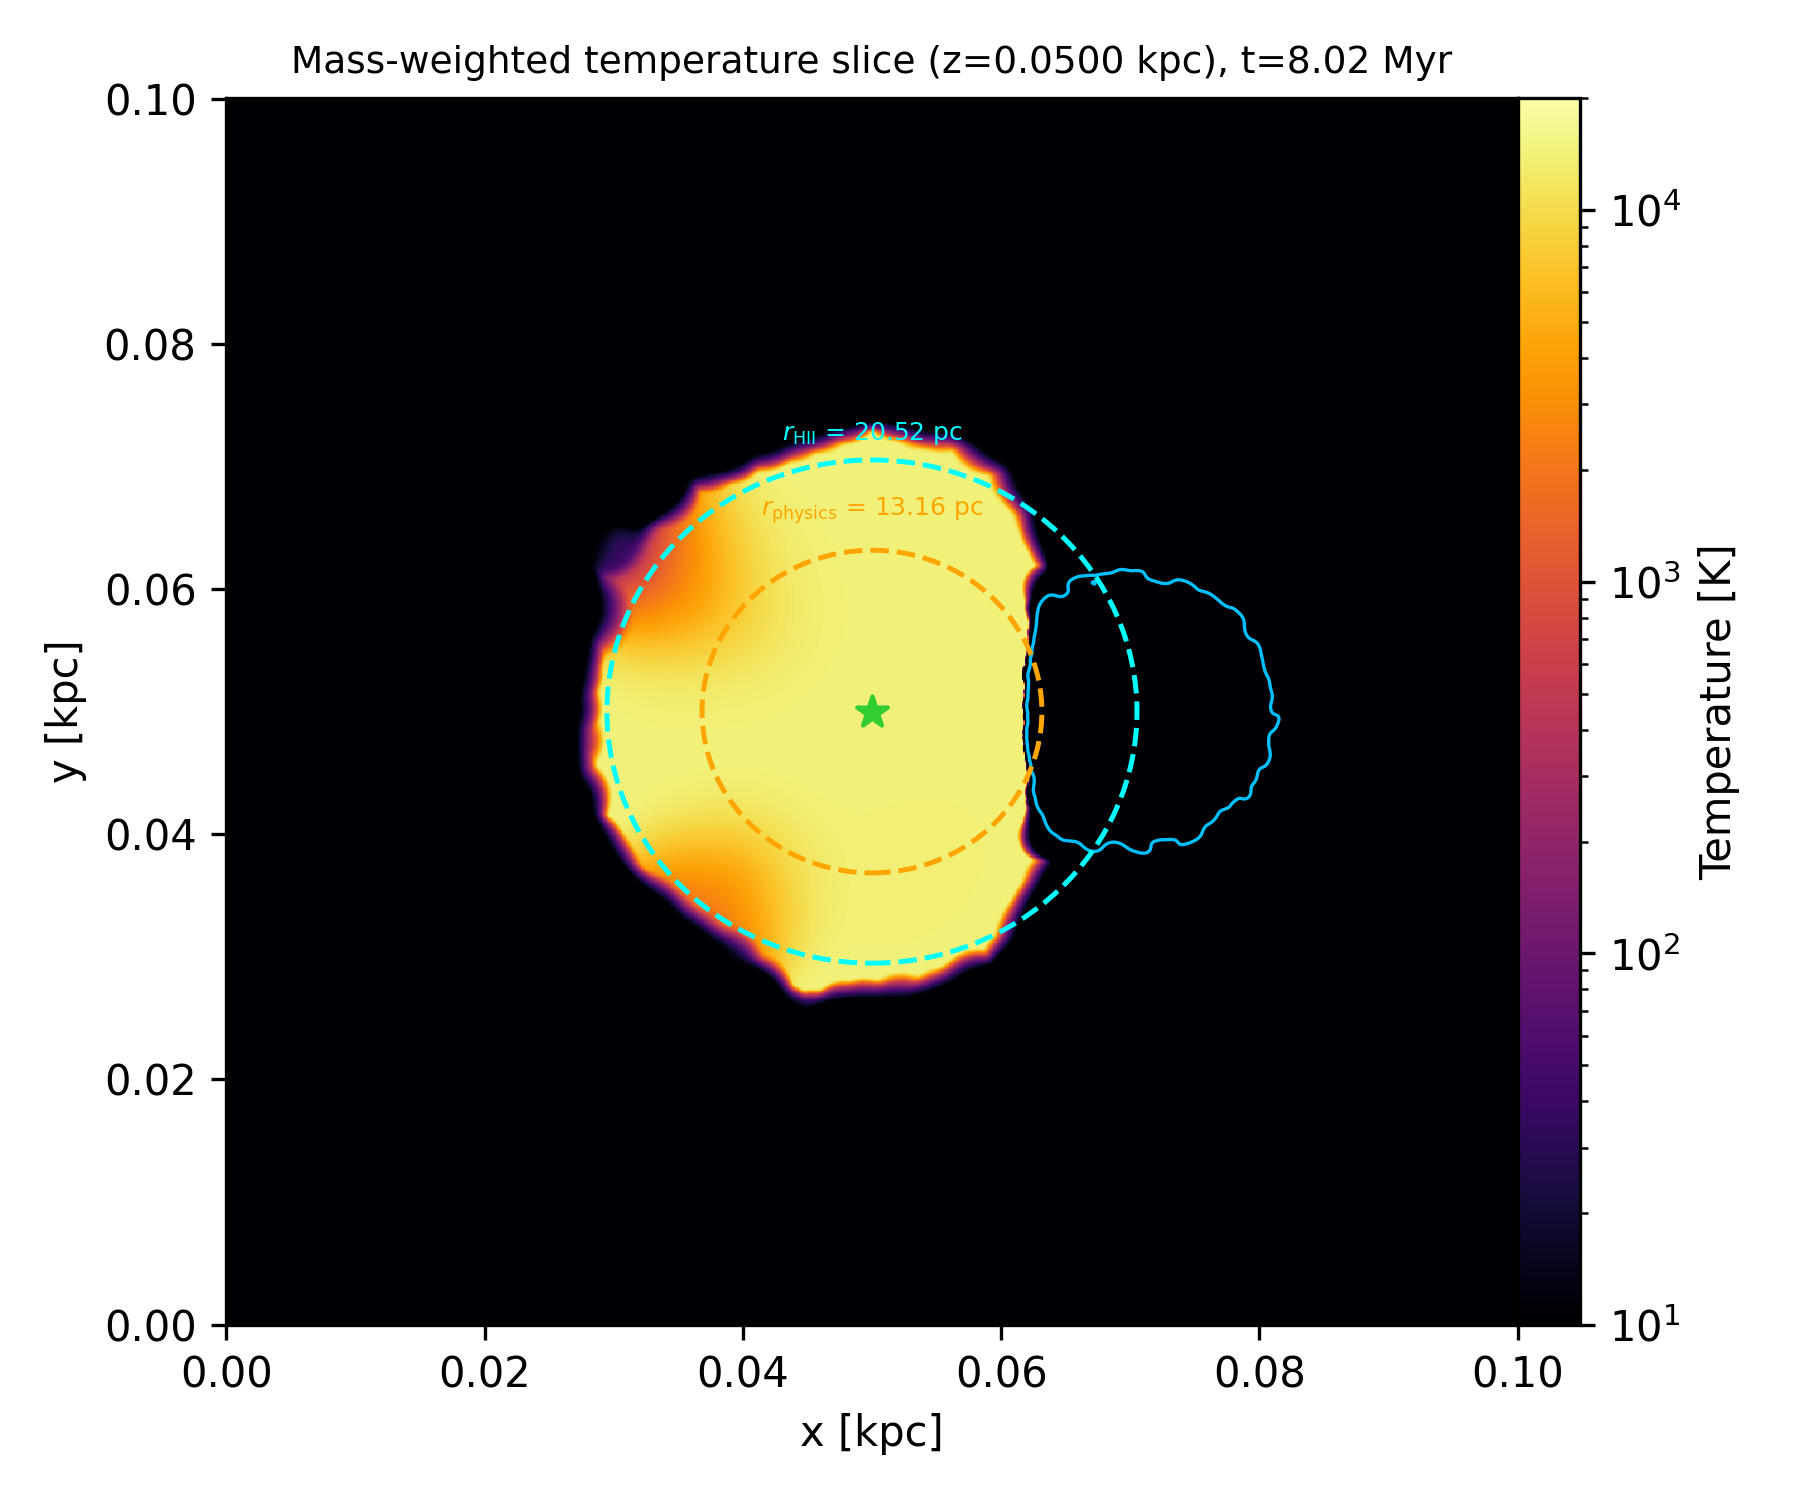
\includegraphics[width=0.325\linewidth]{Figures/tslice_gas20_nside1_rebuild0p05} &
    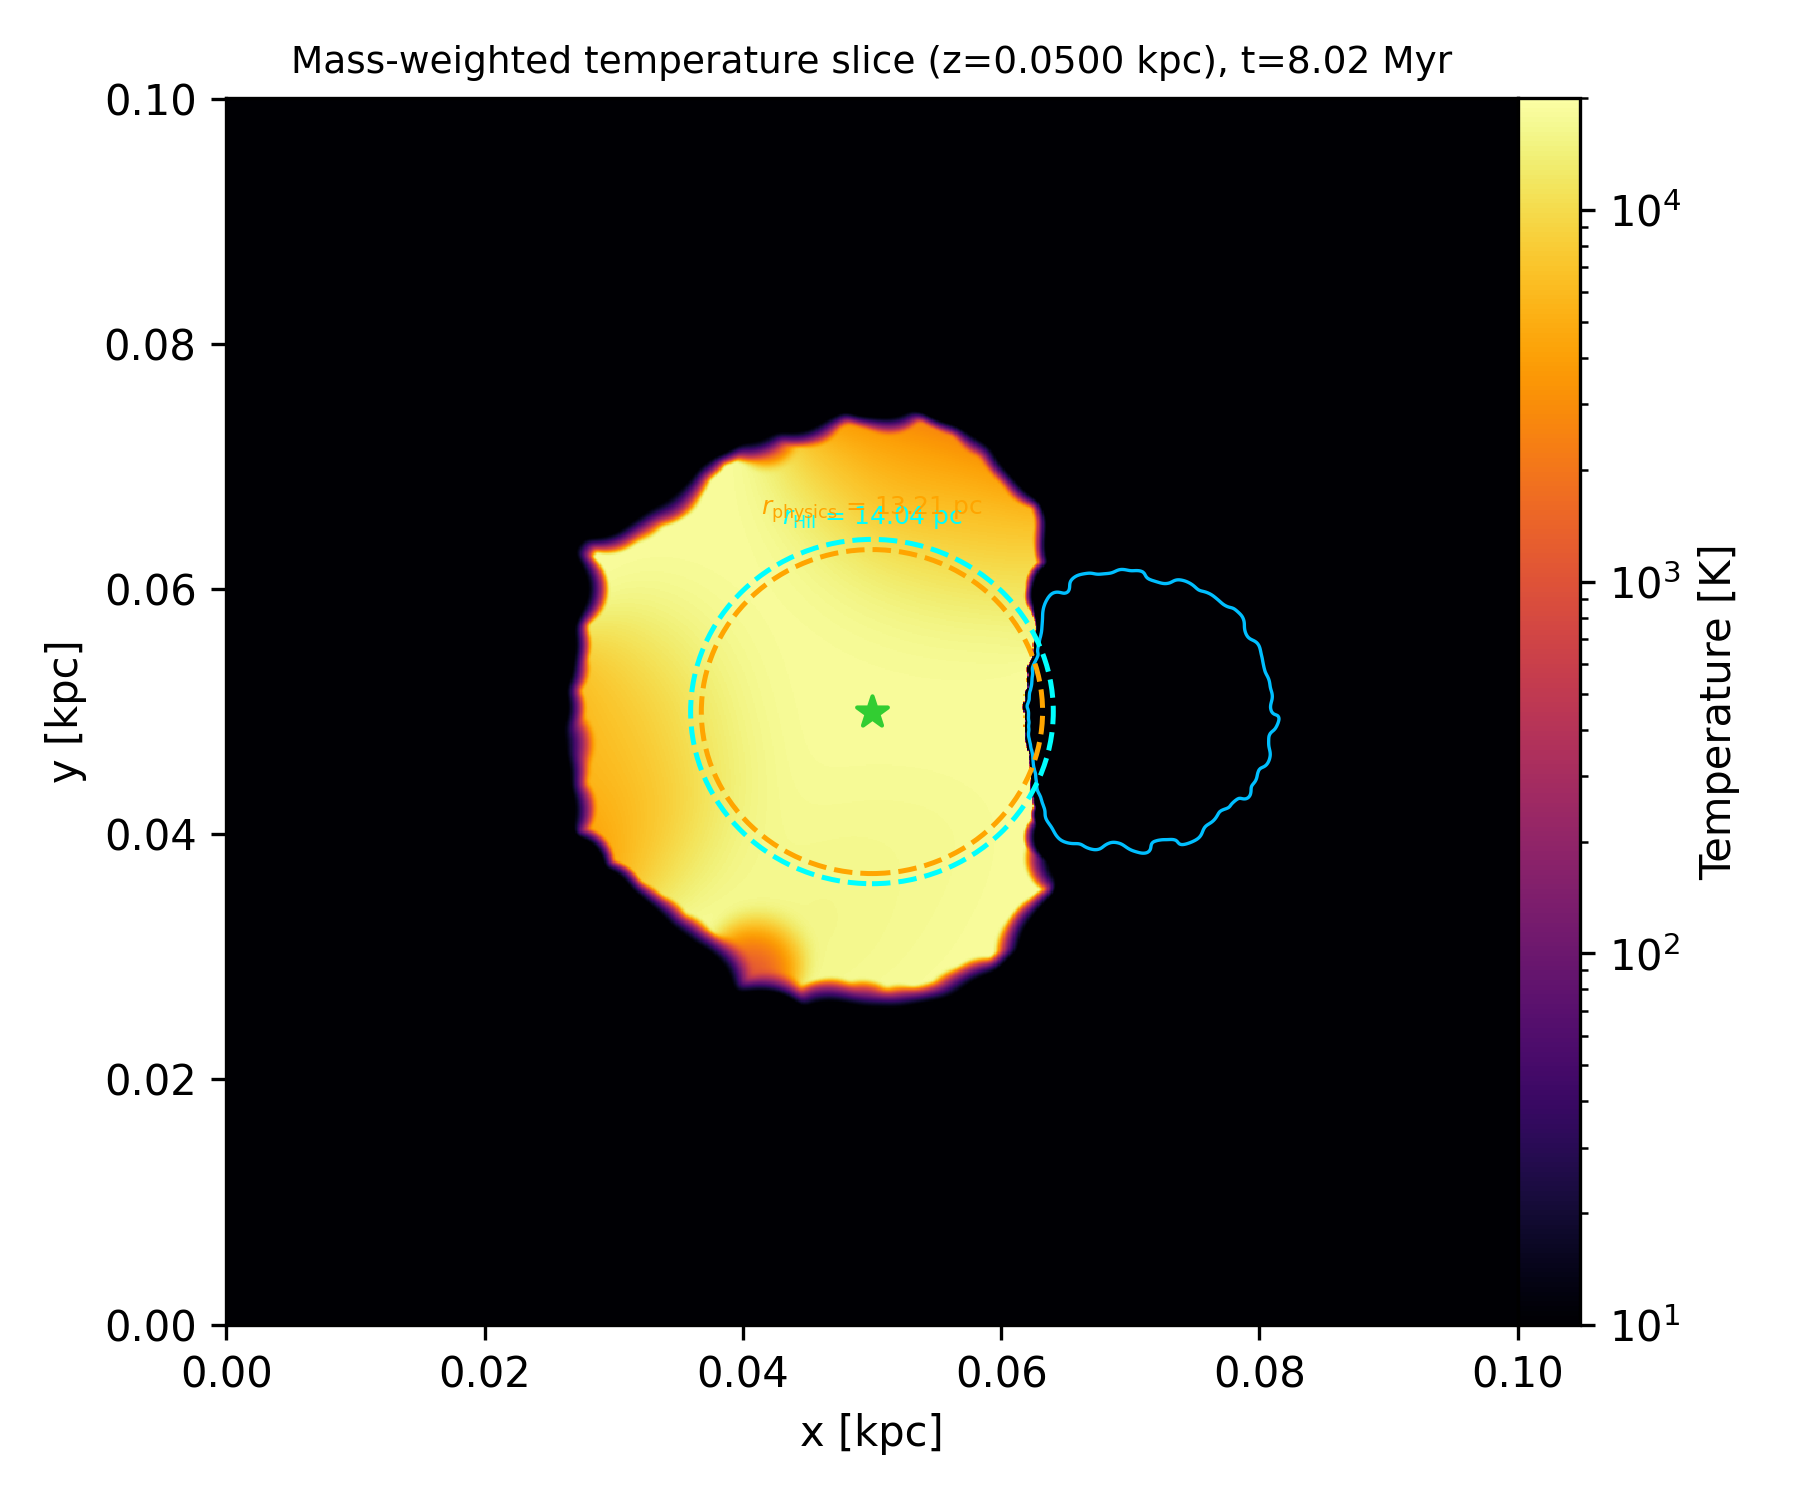
\includegraphics[width=0.325\linewidth]{Figures/tslice_gas20_nside1_rebuild0p1} \\
  \end{tabular}
  \caption{Temperature slices at $t=8\,$Myr, \texttt{gas\_mass=20}.
    Top row: uniform (nside=0), rebuild$\in\{0.01,0.05,0.1\}$\,Myr
    left to right. Bottom row: angular (nside=1), same rebuild order.
    Cyan circle: $r_{\rm HII}$ (algorithm bookkeeping). Orange circle:
    $r_{\rm physics}$ ($T>10^4\,$K). Bottom-left directly reproduces
    \citeauthor{Smith2021}'s Fig.~2 HealPix panel: intact clump,
    asymmetric notch on the near side, symmetric front elsewhere.}
  \label{fig:gas20-slices}
\end{figure}

\subsection{The $Z/Z_\odot\approx0.231$ matrix at \texttt{gas\_mass=95} (zoom-in resolution)}
\label{sec:matrix-gas95}

\begin{center}
\begin{tabular}{lrrr}
  \hline
  scheme  & rebuild=0.01\,Myr & rebuild=0.05\,Myr & rebuild=0.1\,Myr \\
  \hline
  uniform (nside=0) & 14.7--15.7\,pc & 14.0--14.7\,pc & 12.6--14.7\,pc \\
  angular (nside=1) & 16.4--31.1\,pc & 18.0--28.0\,pc & 14.5--15.4\,pc \\
  \hline
\end{tabular}
\end{center}

\textbf{None of the six configurations reliably reaches the papers'
$\sim$20--25\,pc reference at this resolution.} The uniform scheme is
tight and consistent across all three rebuild cadences (12.6--15.7\,pc)
but systematically low -- consistent with the clump's mass-biasing
effect (Section~\ref{sec:angular-splitting}), which the uniform scheme
has no protection against; see Section~\ref{sec:matrix-gas20} for the
same scheme at \code{gas\_mass=20}. The angular scheme's higher raw
numbers are misleading: Figure~\ref{fig:gas95-slices} shows that the
occasional large single-star value (31.1\,pc, 28.0\,pc) is a
\emph{bookkeeping artifact}, not a genuinely larger ionized region --
$r_{\rm physics}$ (the temperature-threshold measurement) stays at
$\approx$14\,pc for those same snapshots, matching the visibly compact
bubble in the slice. At \code{gas\_mass=95} an angular pixel has too
few nearby candidate particles for its budget to be reliably spent
locally; when a pixel's search radius keeps expanding hunting for
affordable particles, it can eventually tag one isolated, far-away
particle, inflating $r_{\rm HII}=h_{\rm hii}\times\gamma_{\rm kernel}$
without a contiguous ionized region actually extending that far. This
is a distinct failure mode from the previously-documented
$r_{\rm HII}$-\emph{understates}-the-truth case
(Section~\ref{sec:matrix-gas20}) -- here it overstates it, and only for
the angular scheme, only at this coarser resolution.

Figure~\ref{fig:gas95-growth} shows the full per-star trajectories.
\textbf{Conclusion: at \code{gas\_mass=95}, this test does not cleanly
reproduce the papers regardless of scheme or rebuild cadence} -- the
uniform scheme under-ionizes consistently, and the angular scheme's
apparent occasional matches are not real. This is itself a useful
result for production use: it says the D-type test in this exact
geometry is not a reliable calibration point at zoom-in resolution, not
that a particular rebuild cadence is preferred over another there.

\begin{figure}
  \centering
  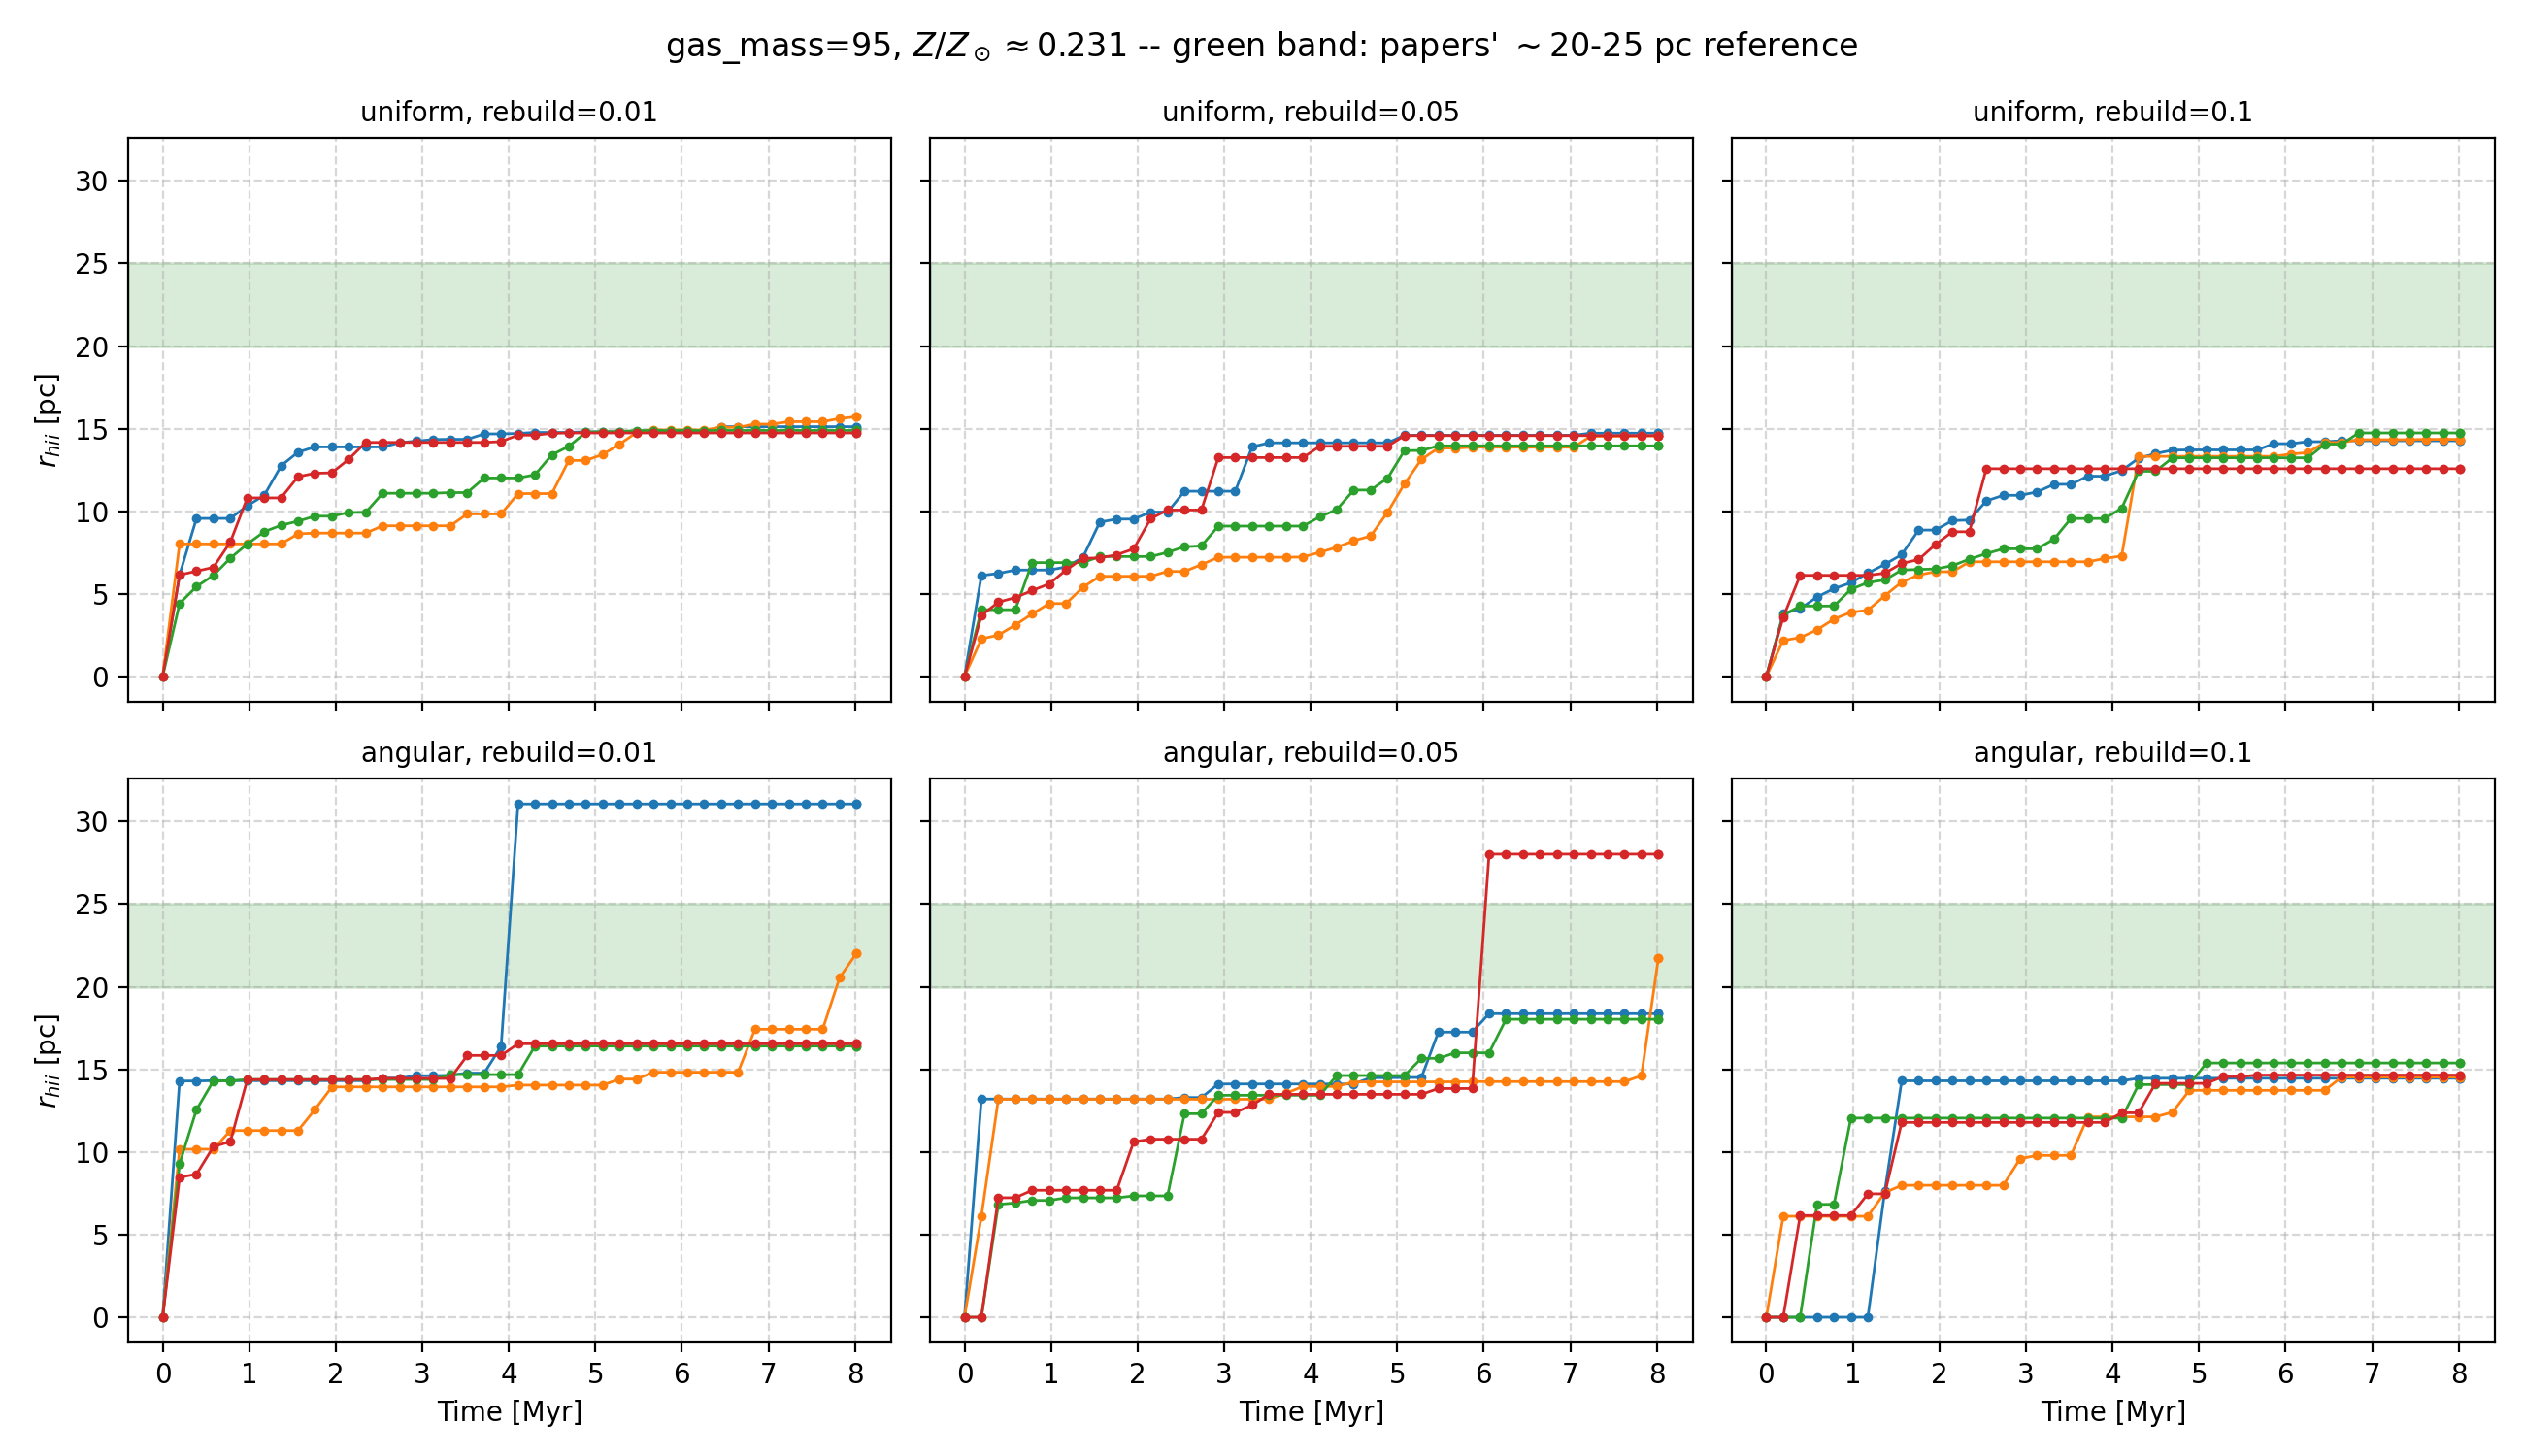
\includegraphics[width=\linewidth]{Figures/gas95_z0231_matrix}
  \caption{Per-star $r_{\rm HII}(t)$ at \texttt{gas\_mass=95},
    $Z/Z_\odot\approx0.231$, for all six configurations. Green band:
    the papers' $\sim$20--25\,pc reference. The occasional large jumps
    in the angular row are bookkeeping artifacts (see text and
    Figure~\ref{fig:gas95-slices}).}
  \label{fig:gas95-growth}
\end{figure}

\begin{figure}
  \centering
  \begin{tabular}{@{}c@{}c@{}c@{}}
    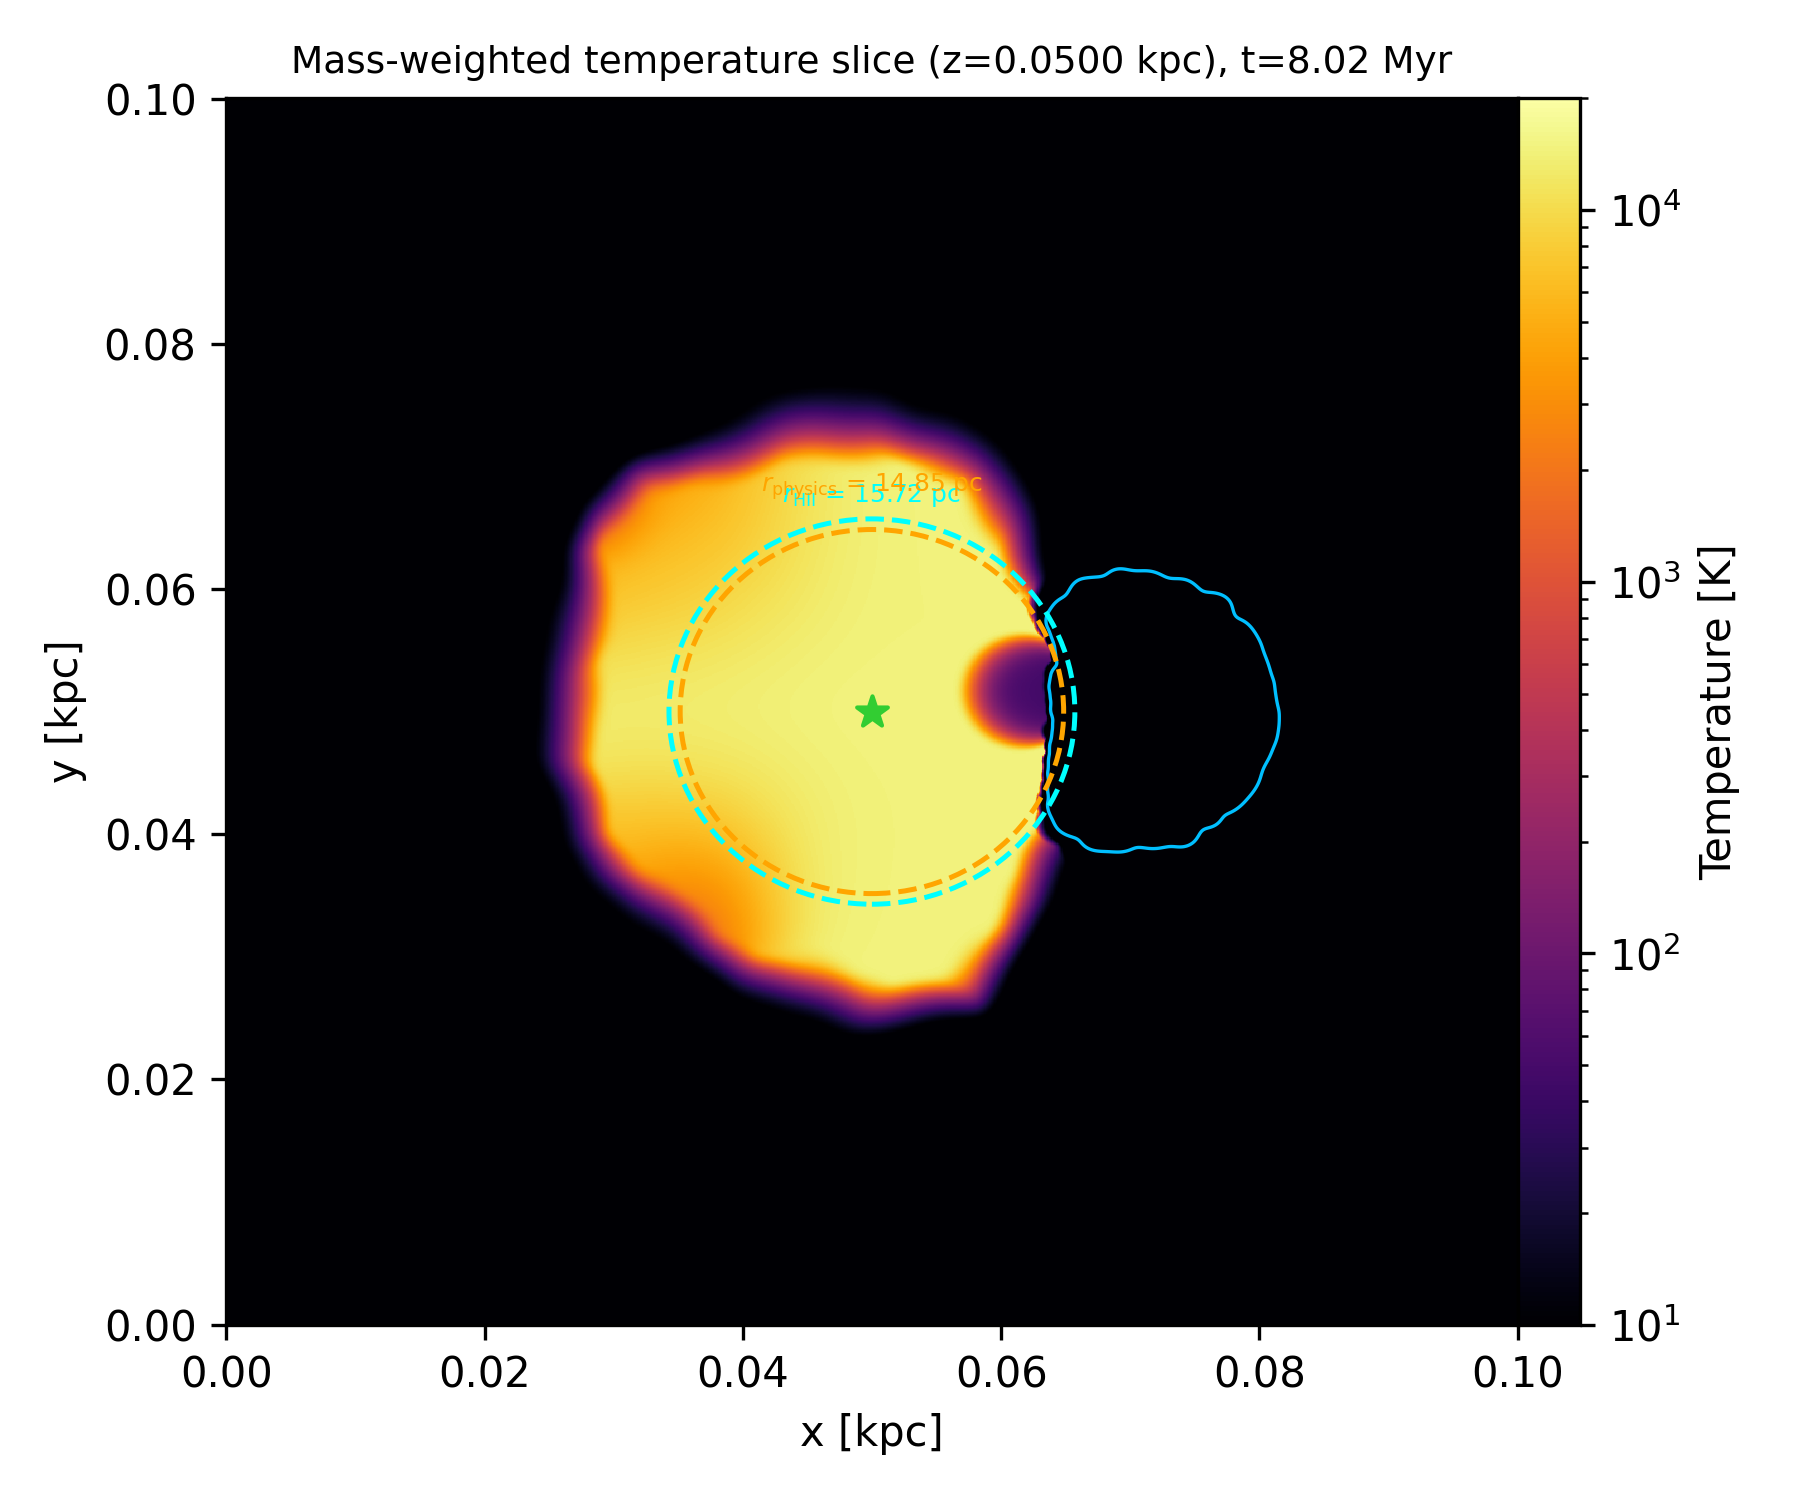
\includegraphics[width=0.325\linewidth]{Figures/tslice_gas95_nside0_rebuild0p01} &
    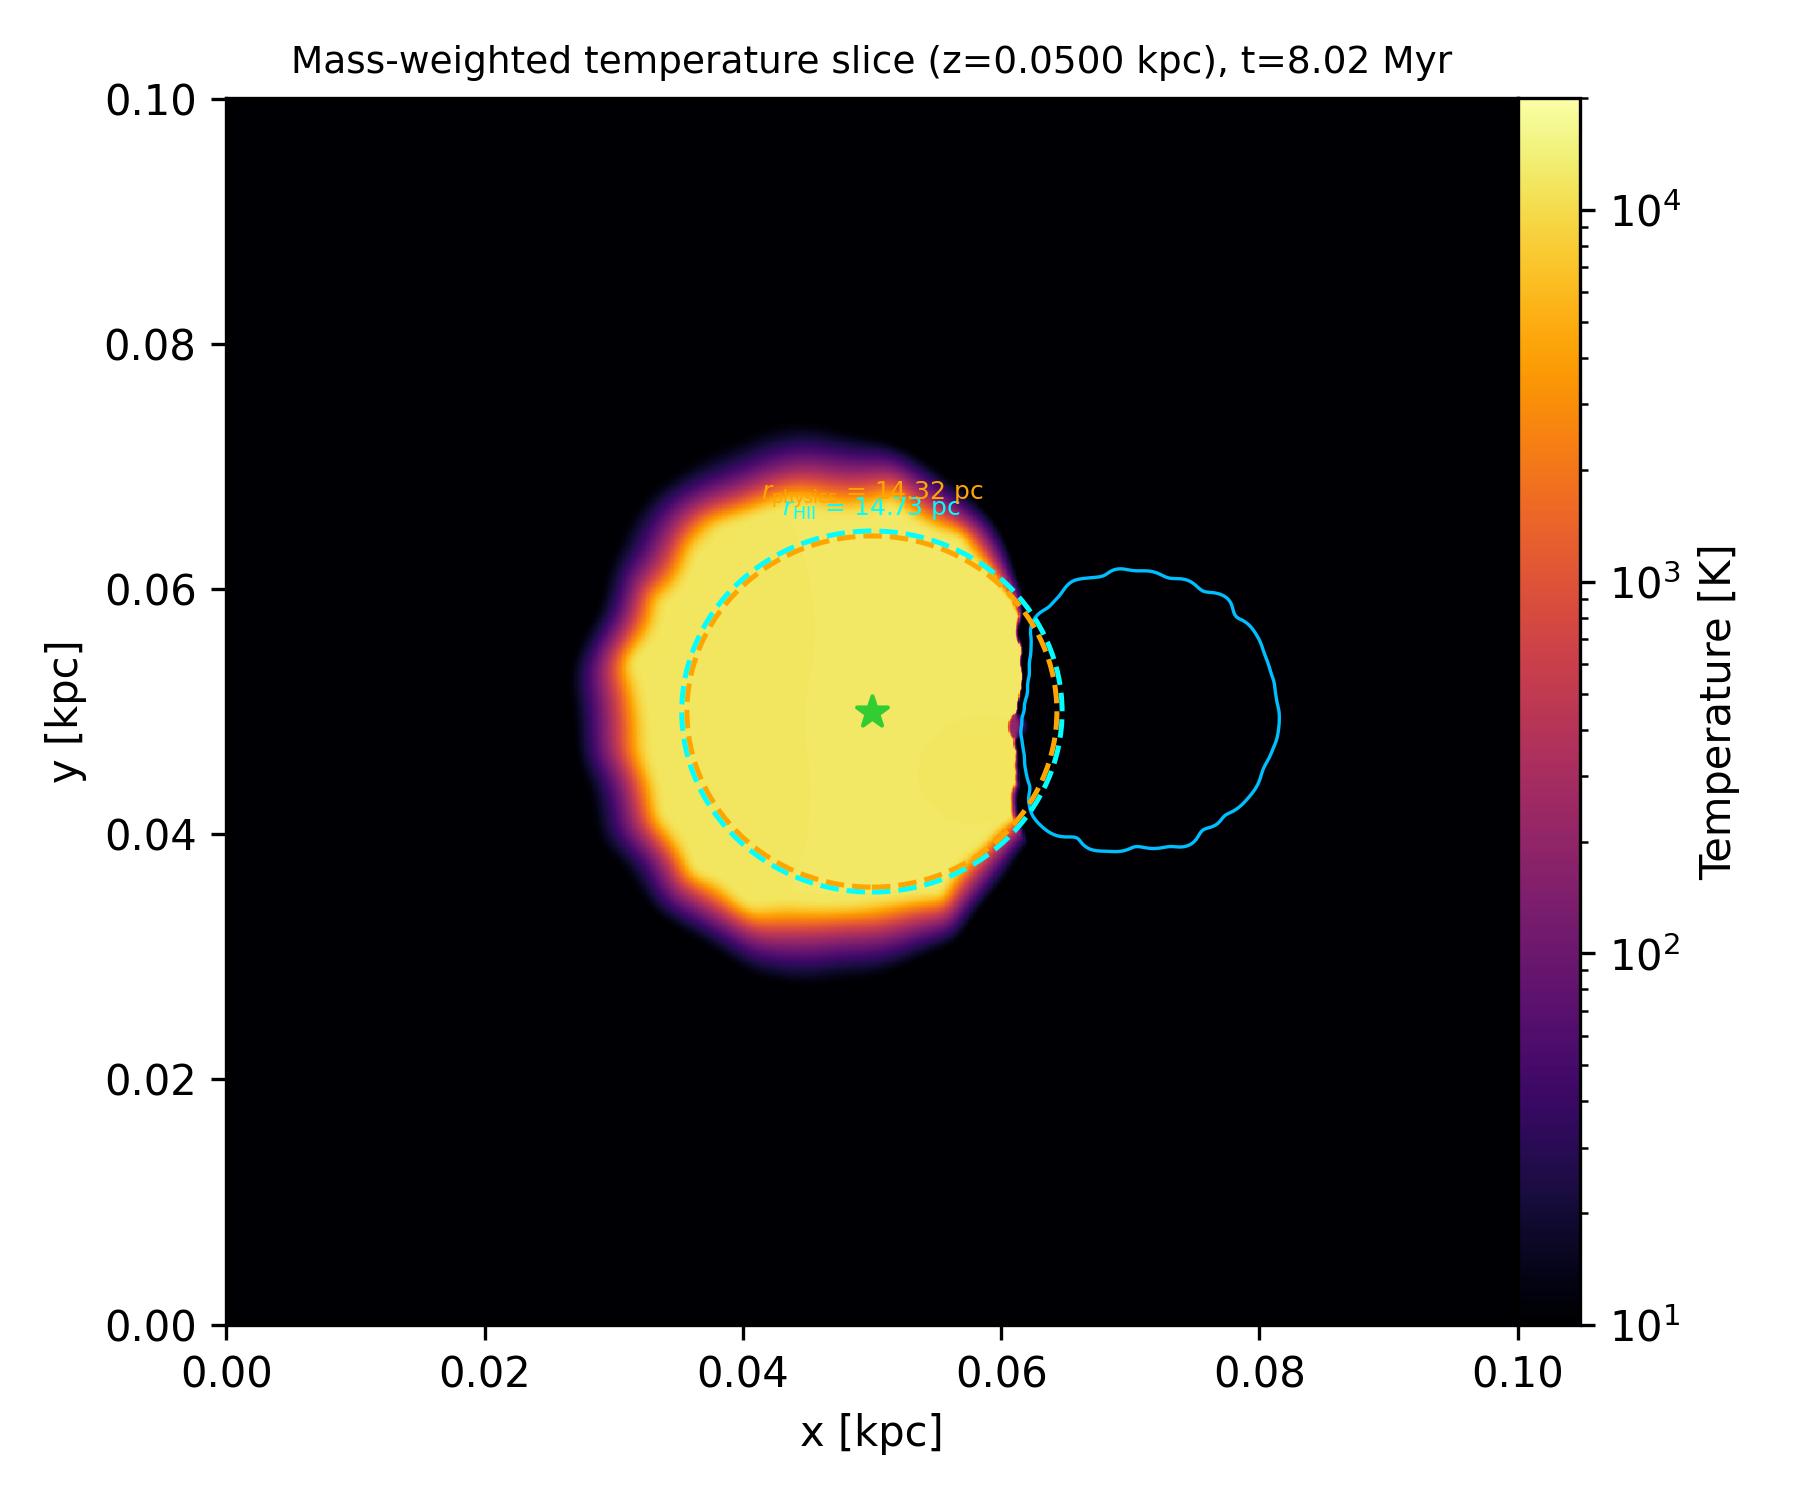
\includegraphics[width=0.325\linewidth]{Figures/tslice_gas95_nside0_rebuild0p05} &
    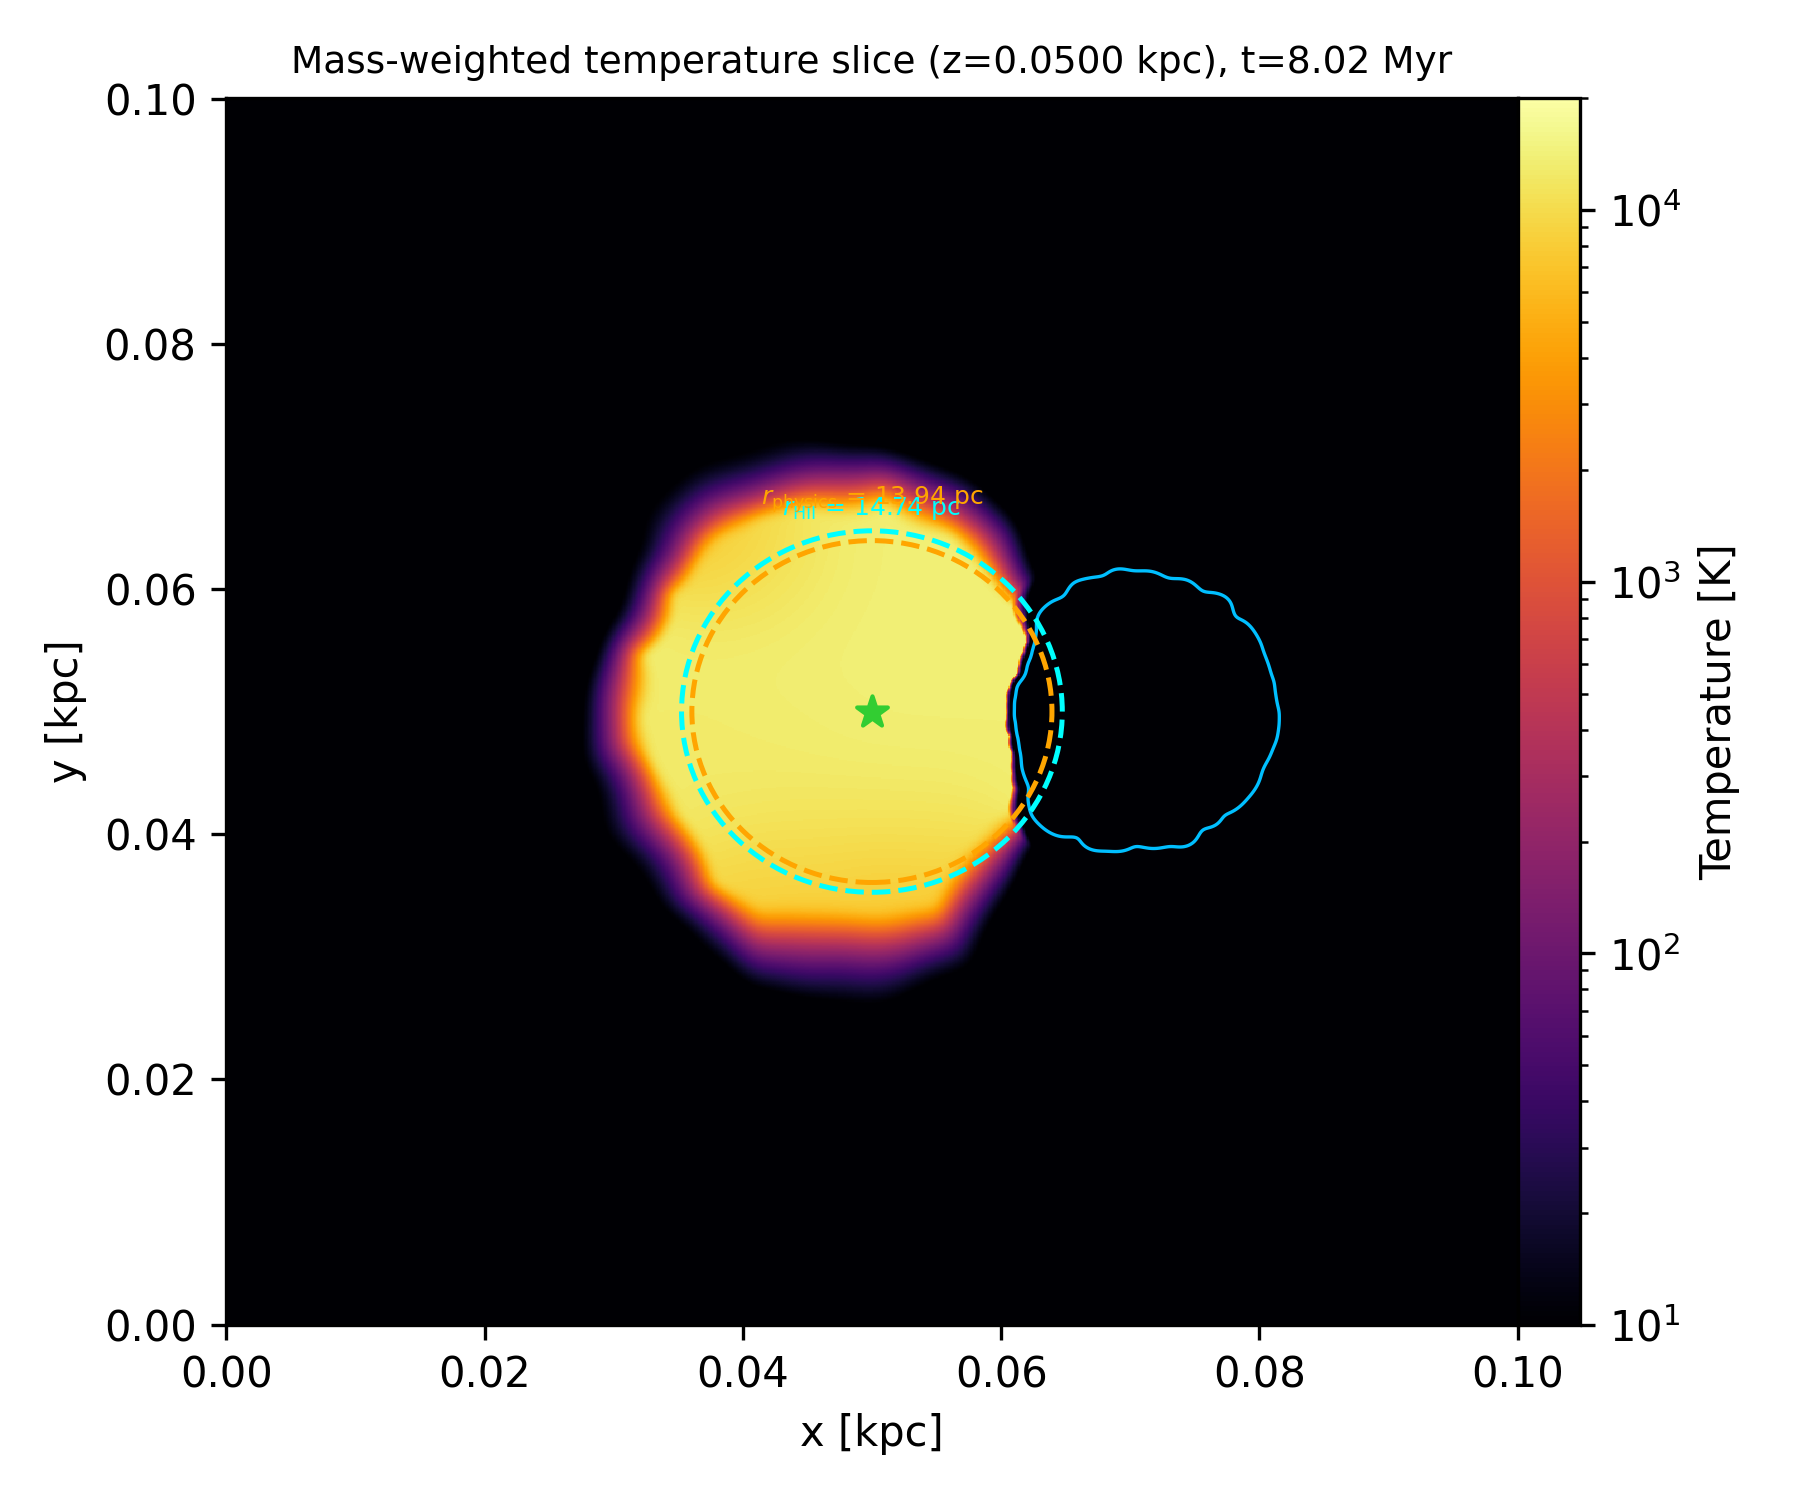
\includegraphics[width=0.325\linewidth]{Figures/tslice_gas95_nside0_rebuild0p1} \\
    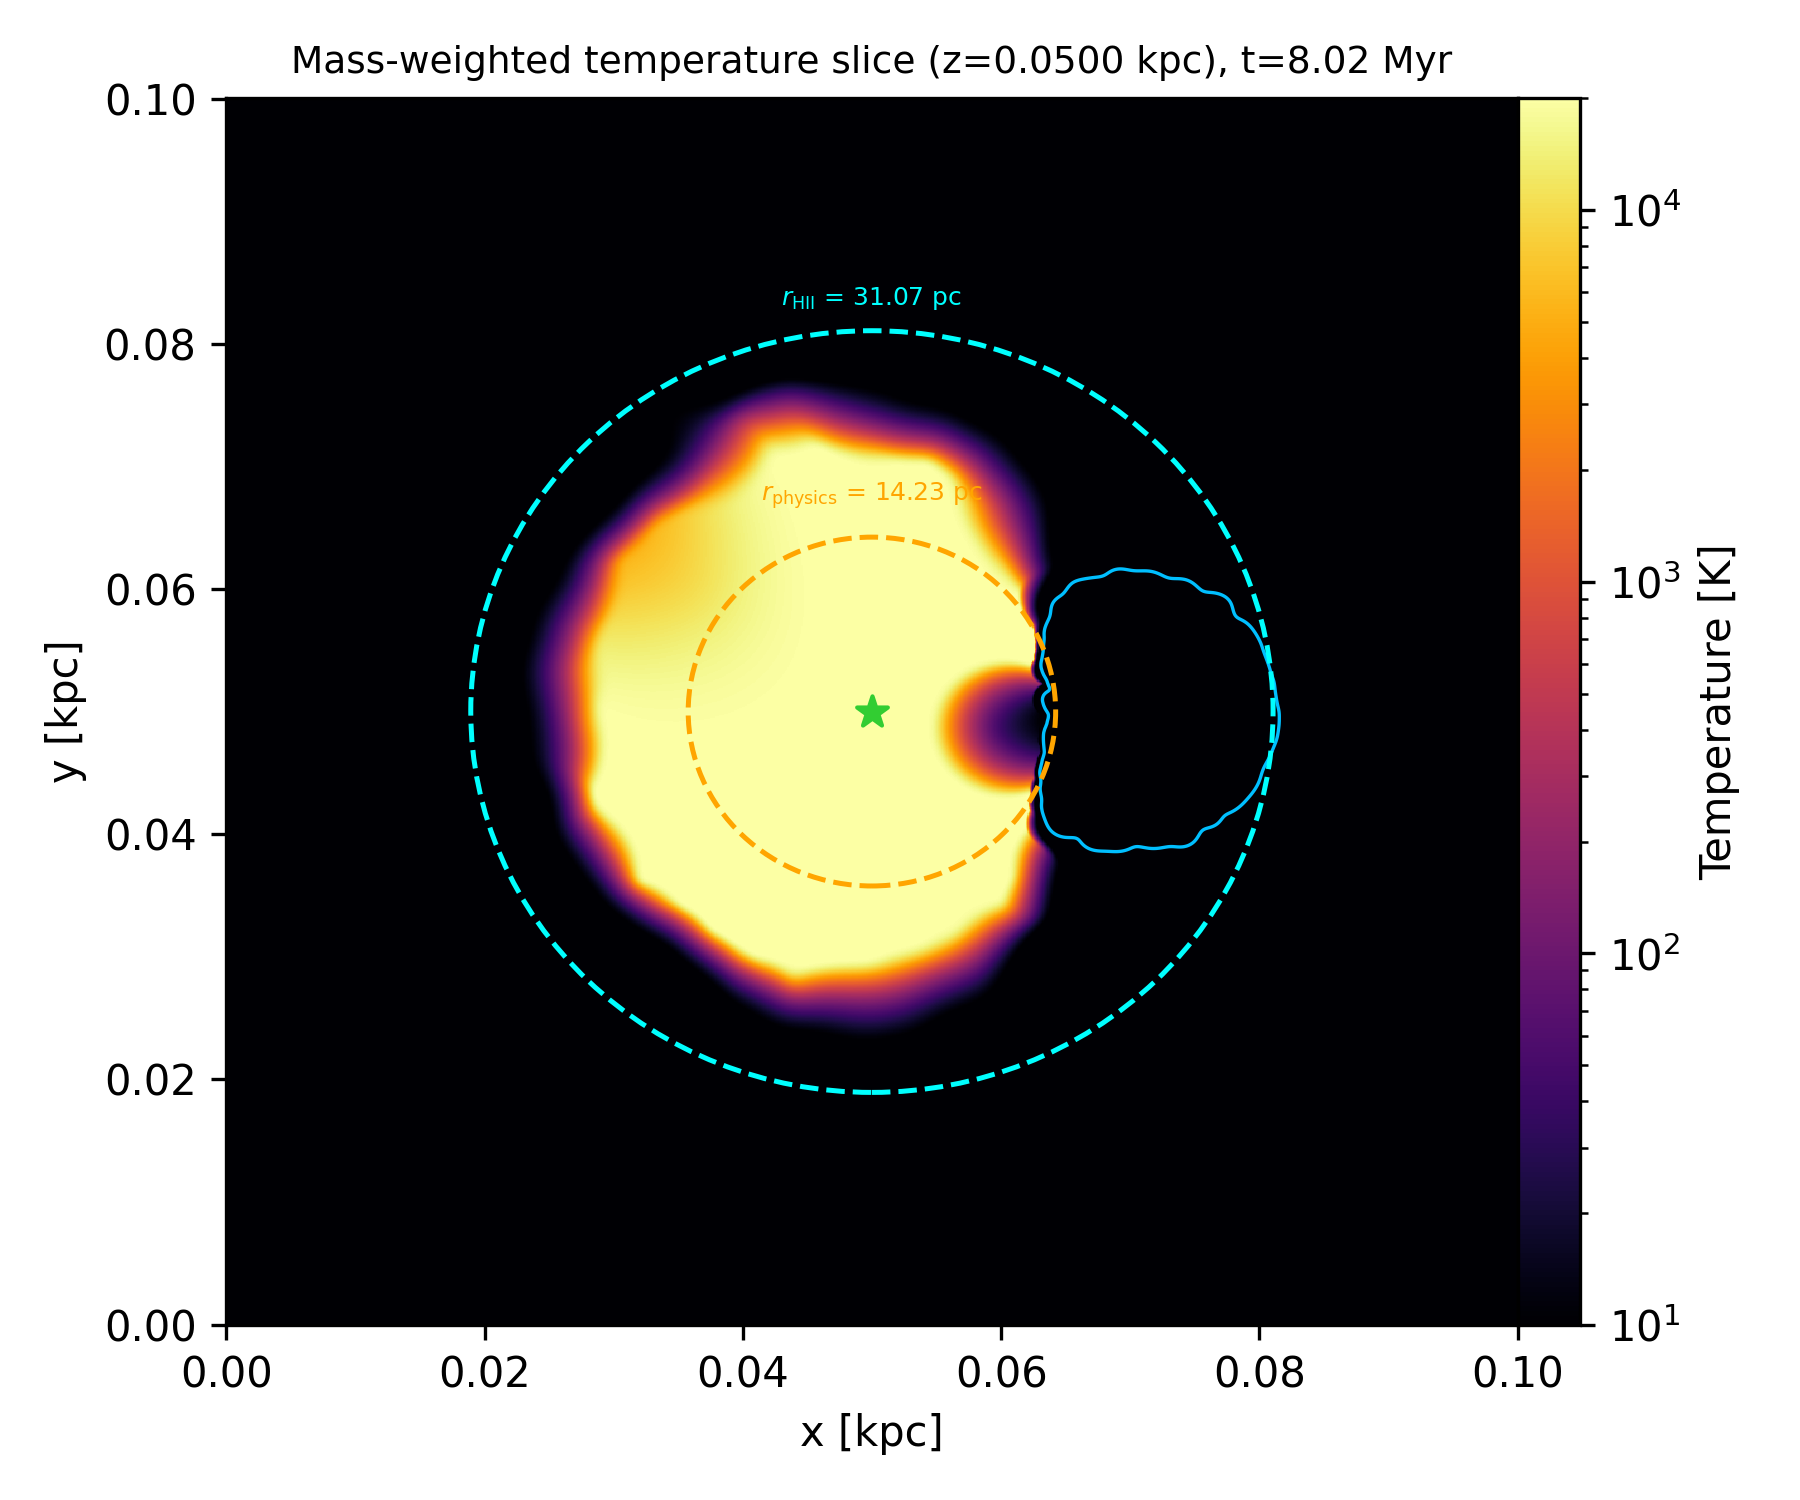
\includegraphics[width=0.325\linewidth]{Figures/tslice_gas95_nside1_rebuild0p01} &
    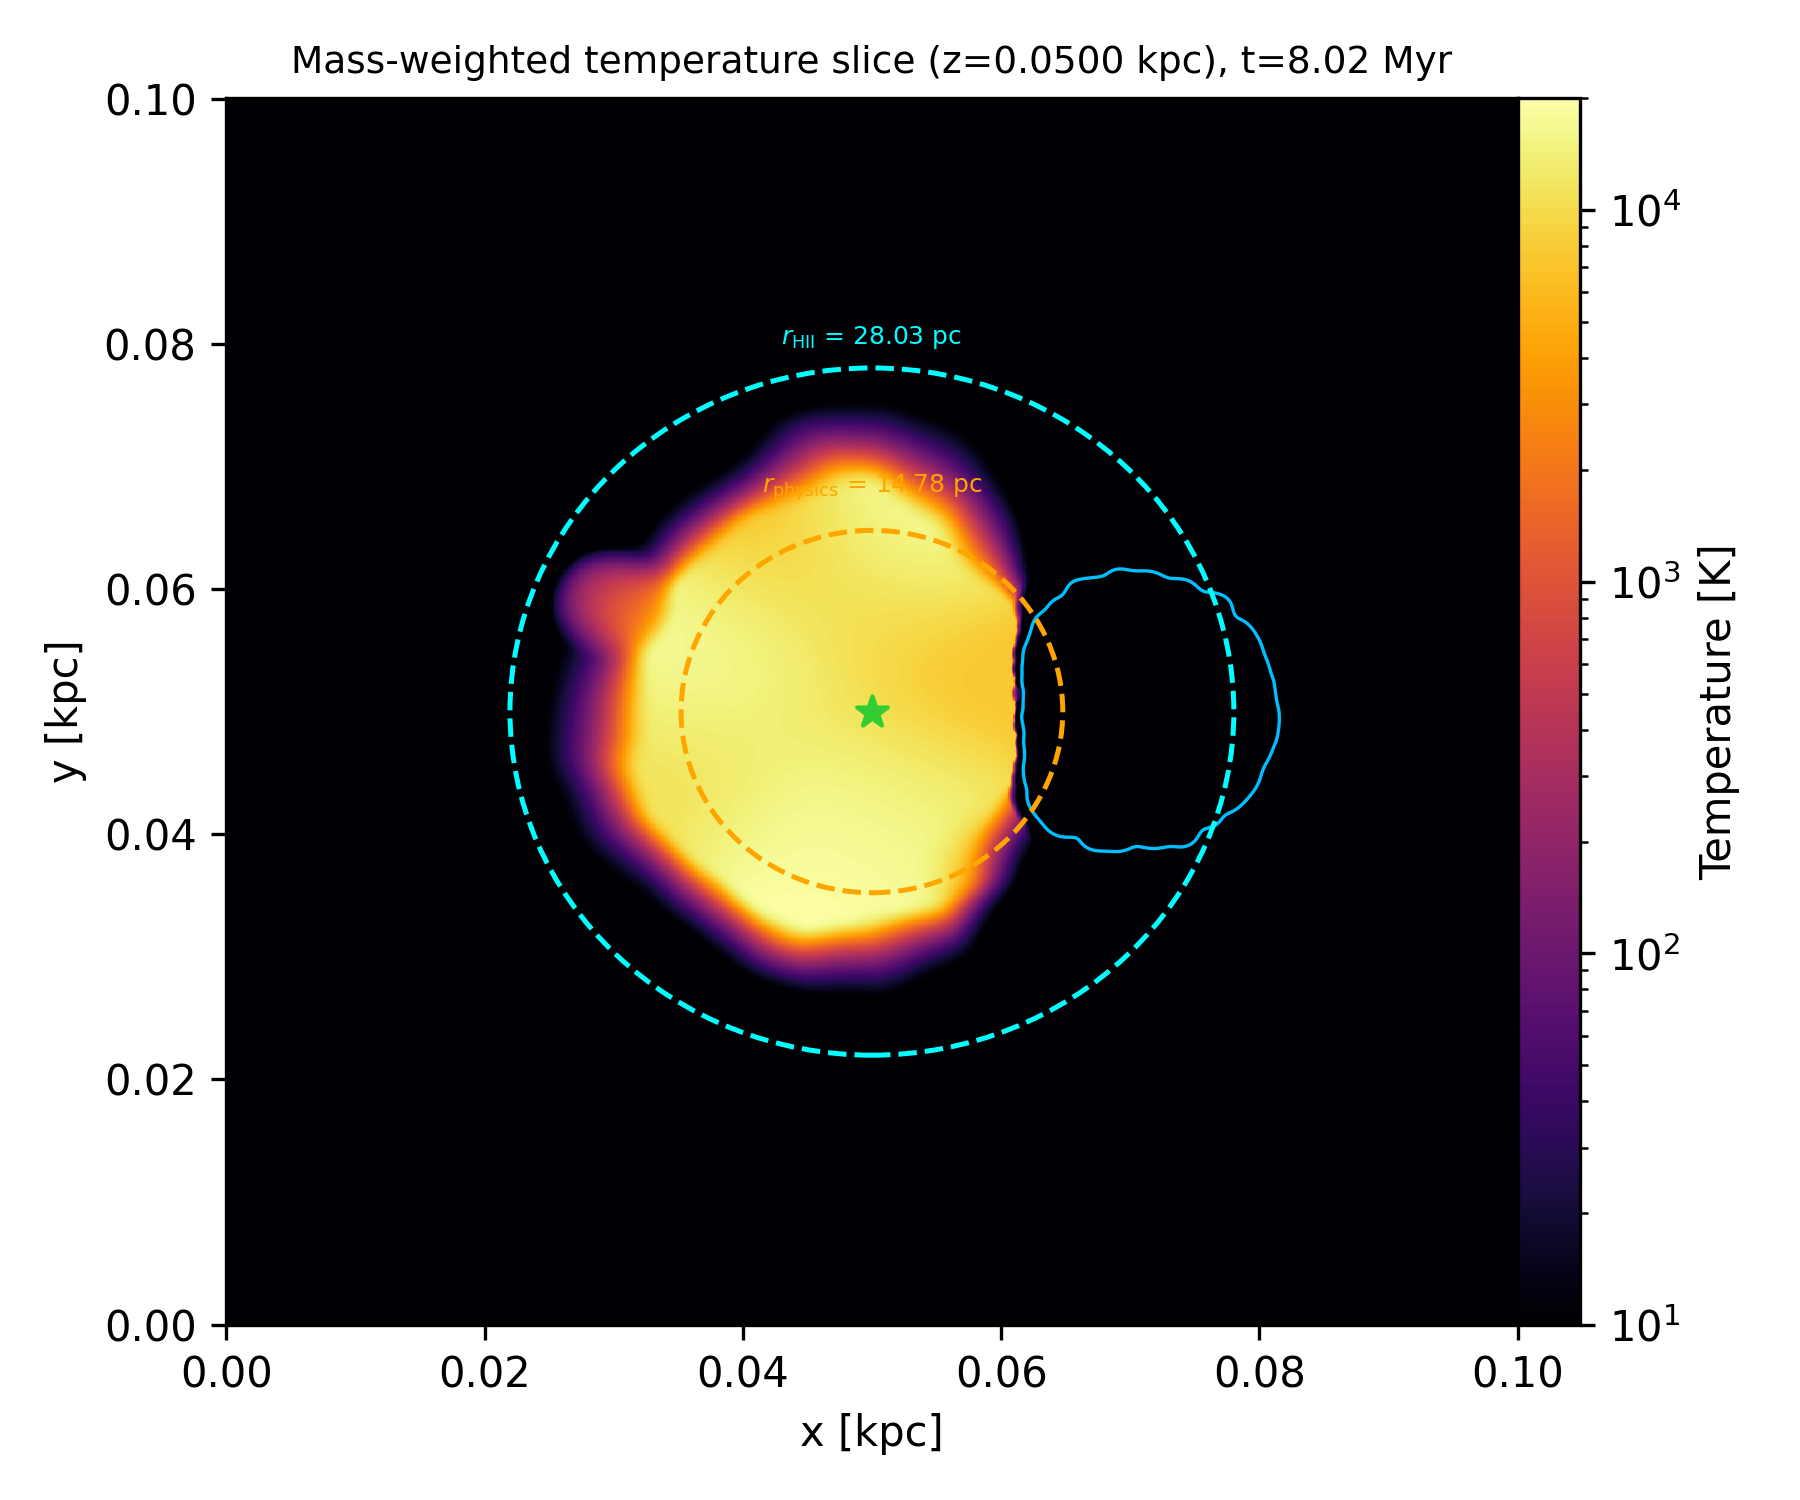
\includegraphics[width=0.325\linewidth]{Figures/tslice_gas95_nside1_rebuild0p05} &
    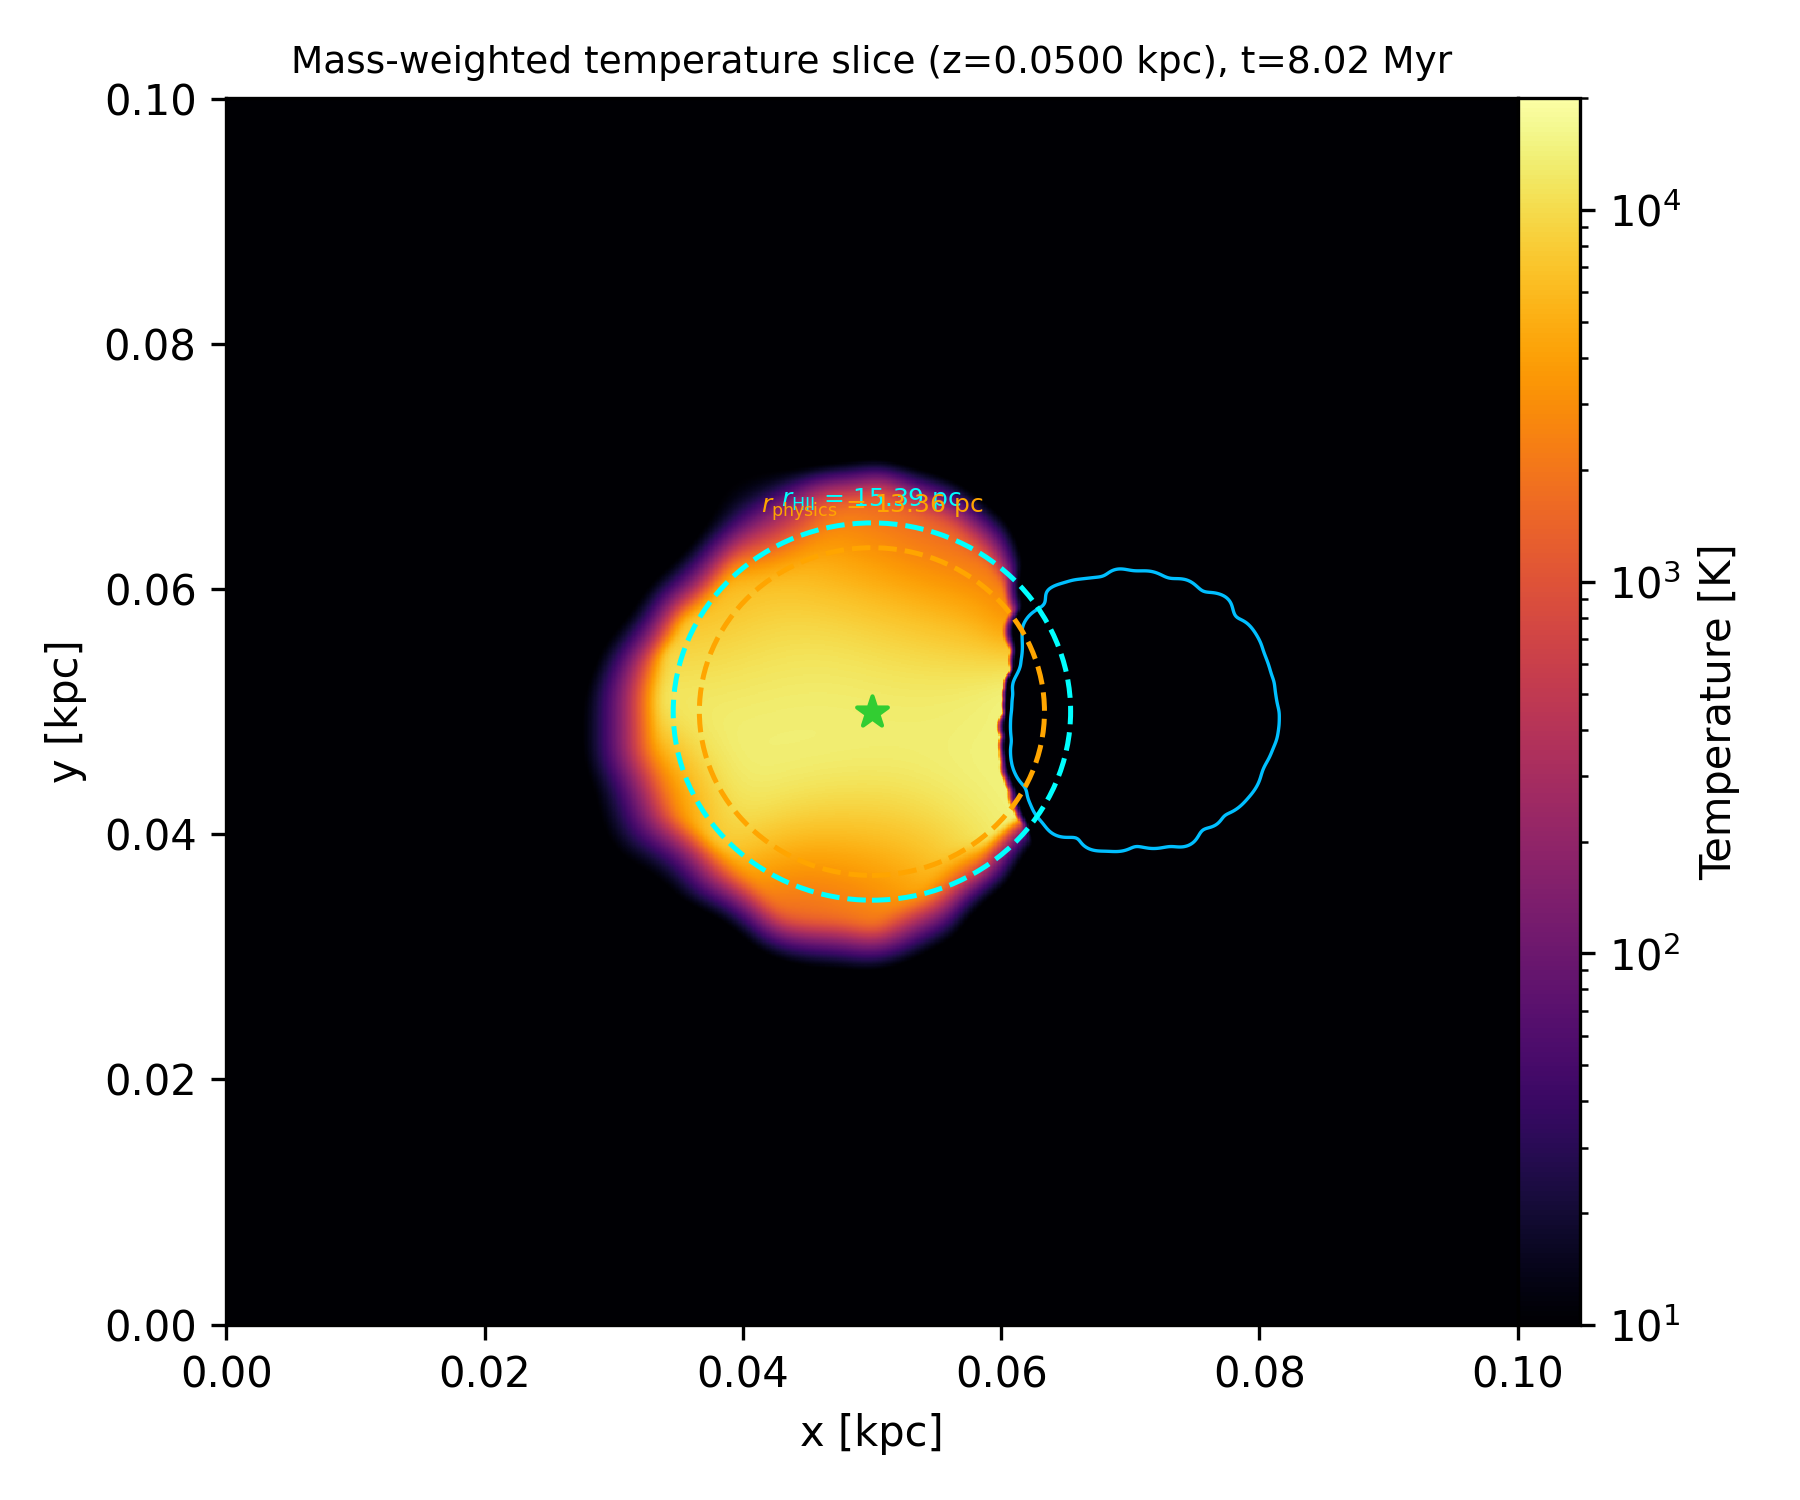
\includegraphics[width=0.325\linewidth]{Figures/tslice_gas95_nside1_rebuild0p1} \\
  \end{tabular}
  \caption{Temperature slices at $t=8\,$Myr, \texttt{gas\_mass=95}.
    Top row: uniform (nside=0), rebuild$\in\{0.01,0.05,0.1\}$\,Myr
    left to right. Bottom row: angular (nside=1), same rebuild order.
    Cyan circle: $r_{\rm HII}$ (algorithm bookkeeping). Orange circle:
    $r_{\rm physics}$ ($T>10^4\,$K). The bottom-left and bottom-middle
    panels show the bookkeeping-artifact cyan circles discussed in the
    text; the orange circles agree closely with the visible bubble in
    all six panels.}
  \label{fig:gas95-slices}
\end{figure}

\subsection{The $Z=0$ matrix (this example's default) -- and why $r_{\rm physics}$ is not trustworthy here}
\label{sec:matrix-z0}

The two matrices above isolate the algorithm from the metallicity
effects in Section~\ref{sec:metallicity} on purpose. For comparison,
here is the same $2\times2\times3$ sweep (both resolutions, both
schemes, all three rebuild cadences) at $Z=0$, this example's actual
default -- deliberately \emph{without} widening
\code{Stars:max\_HII\_search\_radius} or the box, so some rows are
expected to run into the 45\,pc/50\,pc-half-width ceiling; that is an
accepted limitation of this comparison, not a new bug.

\begin{center}
\begin{tabular}{llrrr}
  \hline
  & scheme & rebuild=0.01\,Myr & rebuild=0.05\,Myr & rebuild=0.1\,Myr \\
  \hline
  \multirow{2}{*}{\code{gas\_mass=95}}
    & uniform & 21.0\,pc       & 18.0--18.7\,pc & 17.4--18.0\,pc \\
    & angular & 31.4--40.1\,pc & 18.8--24.2\,pc & 17.3--30.5\,pc \\
  \multirow{2}{*}{\code{gas\_mass=20}}
    & uniform & 21.2\,pc       & 17.5--17.8\,pc & 16.0--16.6\,pc \\
    & angular & 42.3--45.0\,pc\,(capped) & 27.6--32.3\,pc & 31.9--41.2\,pc \\
  \hline
\end{tabular}
\end{center}

\textbf{Two distinct, additive effects are at play here, not one.}
First, a genuine budget effect: at $Z=0$ the temperature floor
(Eq.~\ref{eq:tcollisional}) holds ionized gas at
$T_{\rm collisional}\approx47{,}500\,$K, and
Section~\ref{sec:beta-temperature}'s table shows
$\alpha_B(47{,}500\,{\rm K})$ is $\approx$75\% below
$\alpha_B(10^4\,{\rm K})$ (the value effectively used, via the
temperature floor, at $Z/Z_\odot\approx0.231$). Since the recombination
cost charged per particle (Eq.~\ref{eq:recomb-cost}) scales linearly
with $\beta$, a star's fixed photon budget can hold roughly $4\times$
as many particles ionized simultaneously at $Z=0$ as at
$Z/Z_\odot\approx0.231$ purely from this coefficient, independent of
any cooling physics -- this alone predicts systematically larger
$r_{\rm HII}$ at $Z=0$, exactly what the table above shows relative to
Sections~\ref{sec:matrix-gas20}--\ref{sec:matrix-gas95}. Second, a
cooling-efficiency effect on top of it: \textbf{unlike at
$Z/Z_\odot\approx0.231$, the angular scheme's advantage over uniform
does not collapse at slow rebuild cadences here} -- at
\code{gas\_mass=20}, \code{rebuild=0.1\,Myr} still reaches
31.9--41.2\,pc, comparable to or above \code{rebuild=0.05\,Myr}, not
degraded down to the uniform scheme's $\approx$16\,pc the way it was at
$Z/Z_\odot\approx0.231$ (Section~\ref{sec:matrix-gas20}). The lower
$\beta$ alone does not explain this specific pattern (it would inflate
all rebuild cadences roughly proportionally, not selectively rescue the
slow ones) -- this part is consistent with the cooling-efficiency
hypothesis instead: at $Z=0$, cooling is inefficient enough that the
pixel-starvation effect is less punishing, because gas that was ionized
earlier stays hot for longer regardless of whether its tag has been
refreshed. The uniform scheme itself is also not yet converged at
$t=8\,$Myr, unlike at $Z/Z_\odot\approx0.231$ where it plateaus by
$t\sim3$--4\,Myr -- Figure~\ref{fig:gas20-z0-growth} shows all six
\code{gas\_mass=20} trajectories still rising at the end of the run.

\textbf{A more important finding: $r_{\rm physics}$ is not a reliable
diagnostic at $Z=0$.} Figure~\ref{fig:z0-vs-z0231-slice} compares the
same configuration (\code{gas\_mass=20}, uniform, rebuild=0.01\,Myr) at
both metallicities. At $Z/Z_\odot\approx0.231$ (left), the background
outside the bubble is completely black -- efficient metal-line cooling
returns any perturbed gas to the ambient $10^3\,$K background quickly,
so $T>10^4\,$K cleanly isolates the photoionized region and $r_{\rm
physics}=14.74\,$pc closely tracks $r_{\rm HII}=14.28\,$pc. At $Z=0$
(right), the \emph{entire box} glows well above the background
temperature -- $r_{\rm physics}=44.87\,$pc, more than double
$r_{\rm HII}=21.25\,$pc, and this pattern repeats for every $Z=0$
configuration tested (see the $r_{\rm HII}$/$r_{\rm physics}$ values
printed by \code{plot\_temperature\_hii.py} for each run). This is not
a bookkeeping artifact of the kind found in
Section~\ref{sec:matrix-gas95} (an isolated far tagged particle) --
the heating is genuinely widespread. The most likely explanation:
inefficient cooling at $Z=0$ lets gas heated by the D-type shock's
swept-up shell, or gas that cooled only partway after its ionization
tag expired, stay above the $10^4\,$K threshold far from the actual
photoionized front and for a long time, exactly the mechanism raised
as a candidate for the angular scheme's rebuild-cadence insensitivity
above. \textbf{Practical consequence: at $Z=0$, $r_{\rm HII}$ (despite
its own known limitations, Section~\ref{sec:matrix-gas20}) is the more
trustworthy of the two diagnostics; $r_{\rm physics}$ should not be
used to validate $Z=0$ runs against the papers' reference without
correcting for this contamination first -- not attempted here.}

\begin{figure}
  \centering
  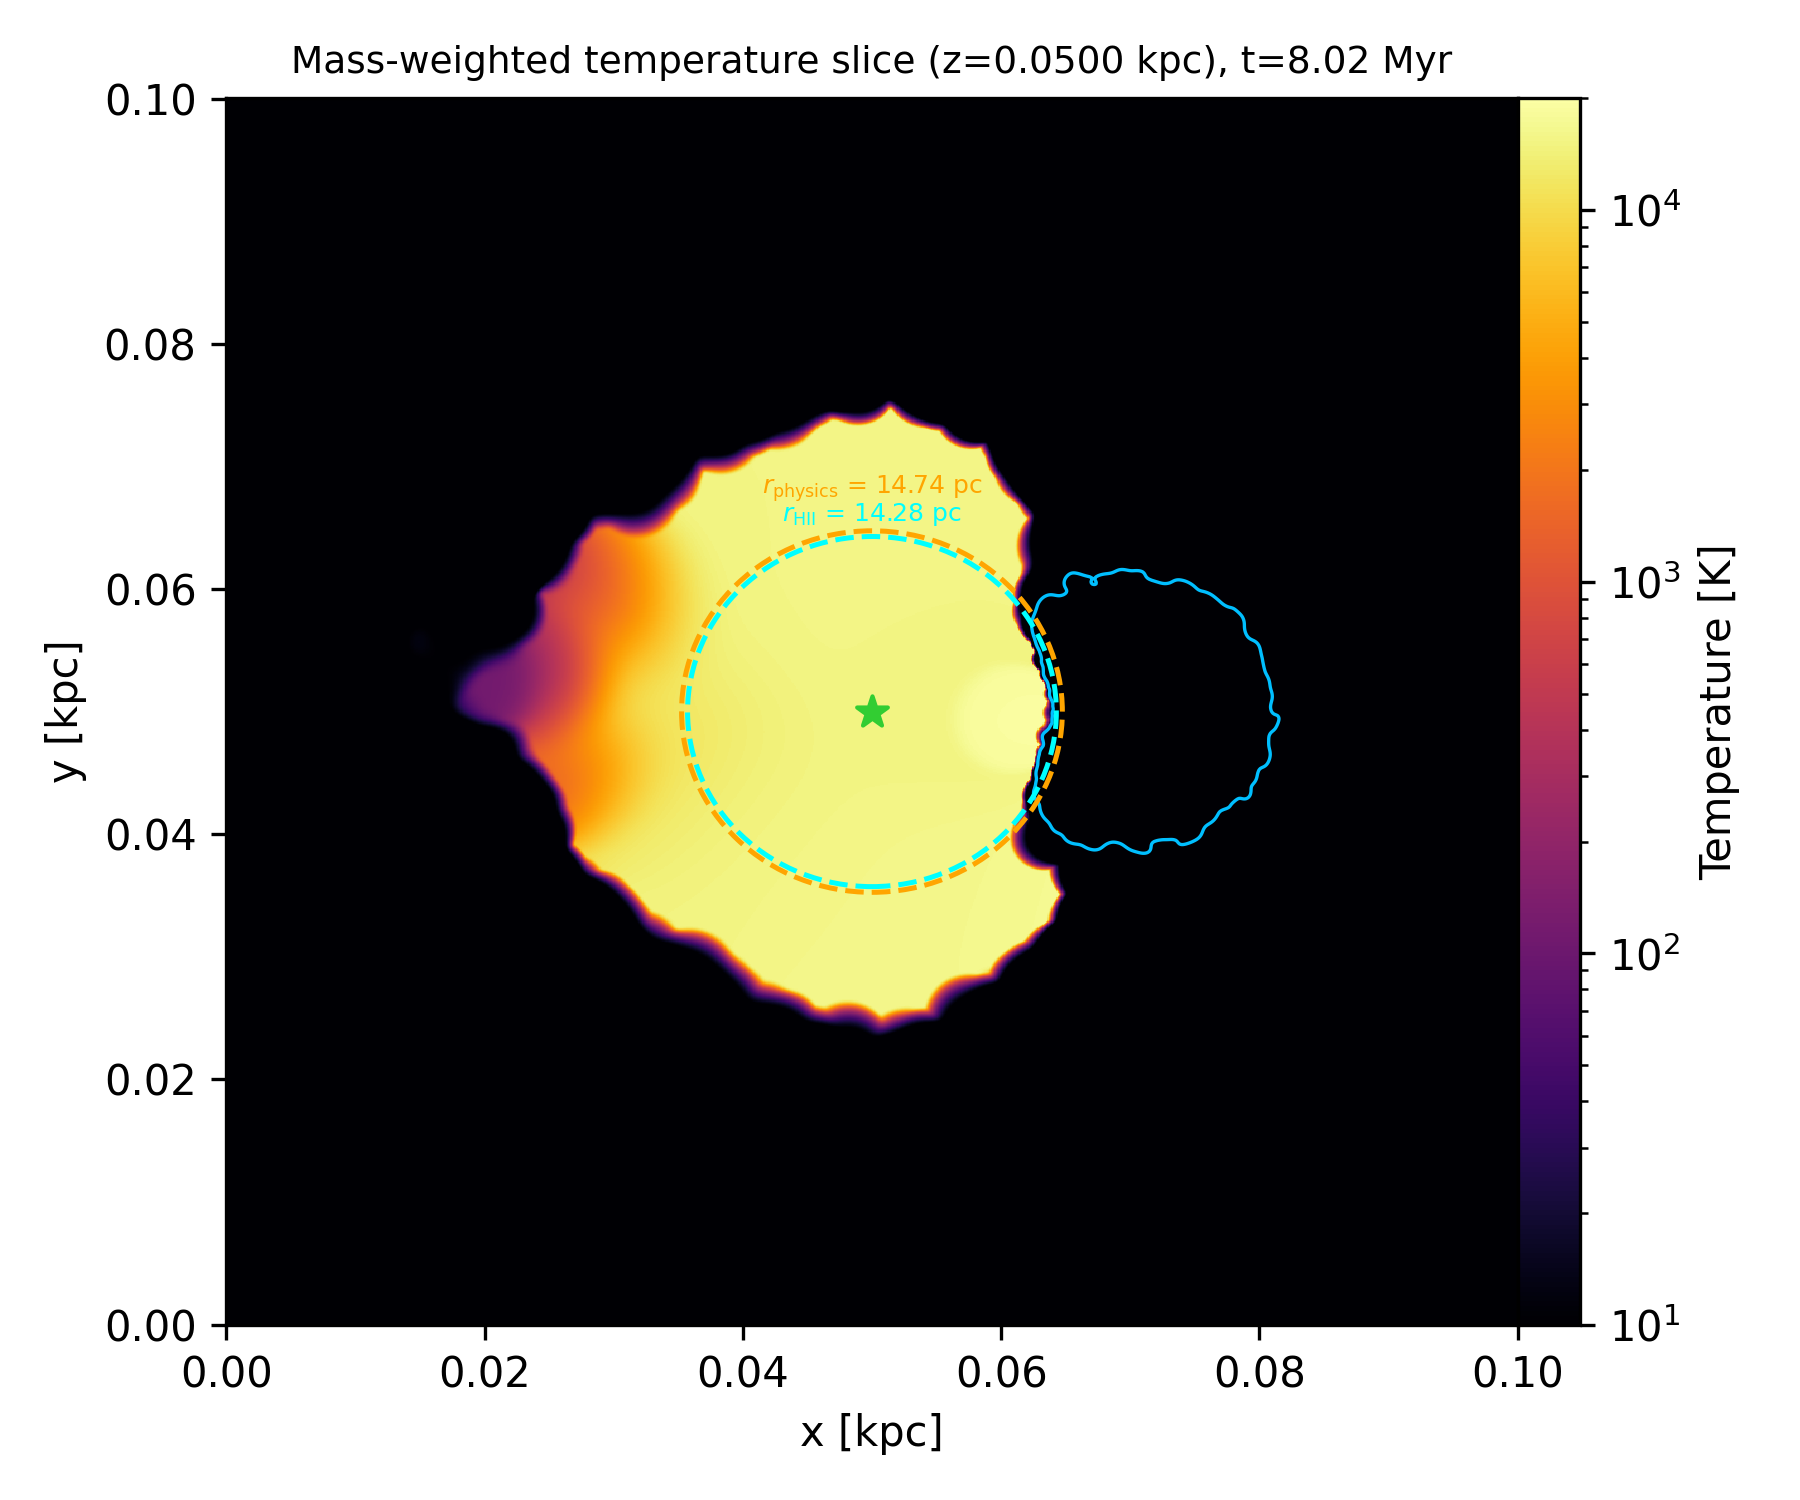
\includegraphics[width=0.48\linewidth]{Figures/tslice_gas20_nside0_rebuild0p01}
  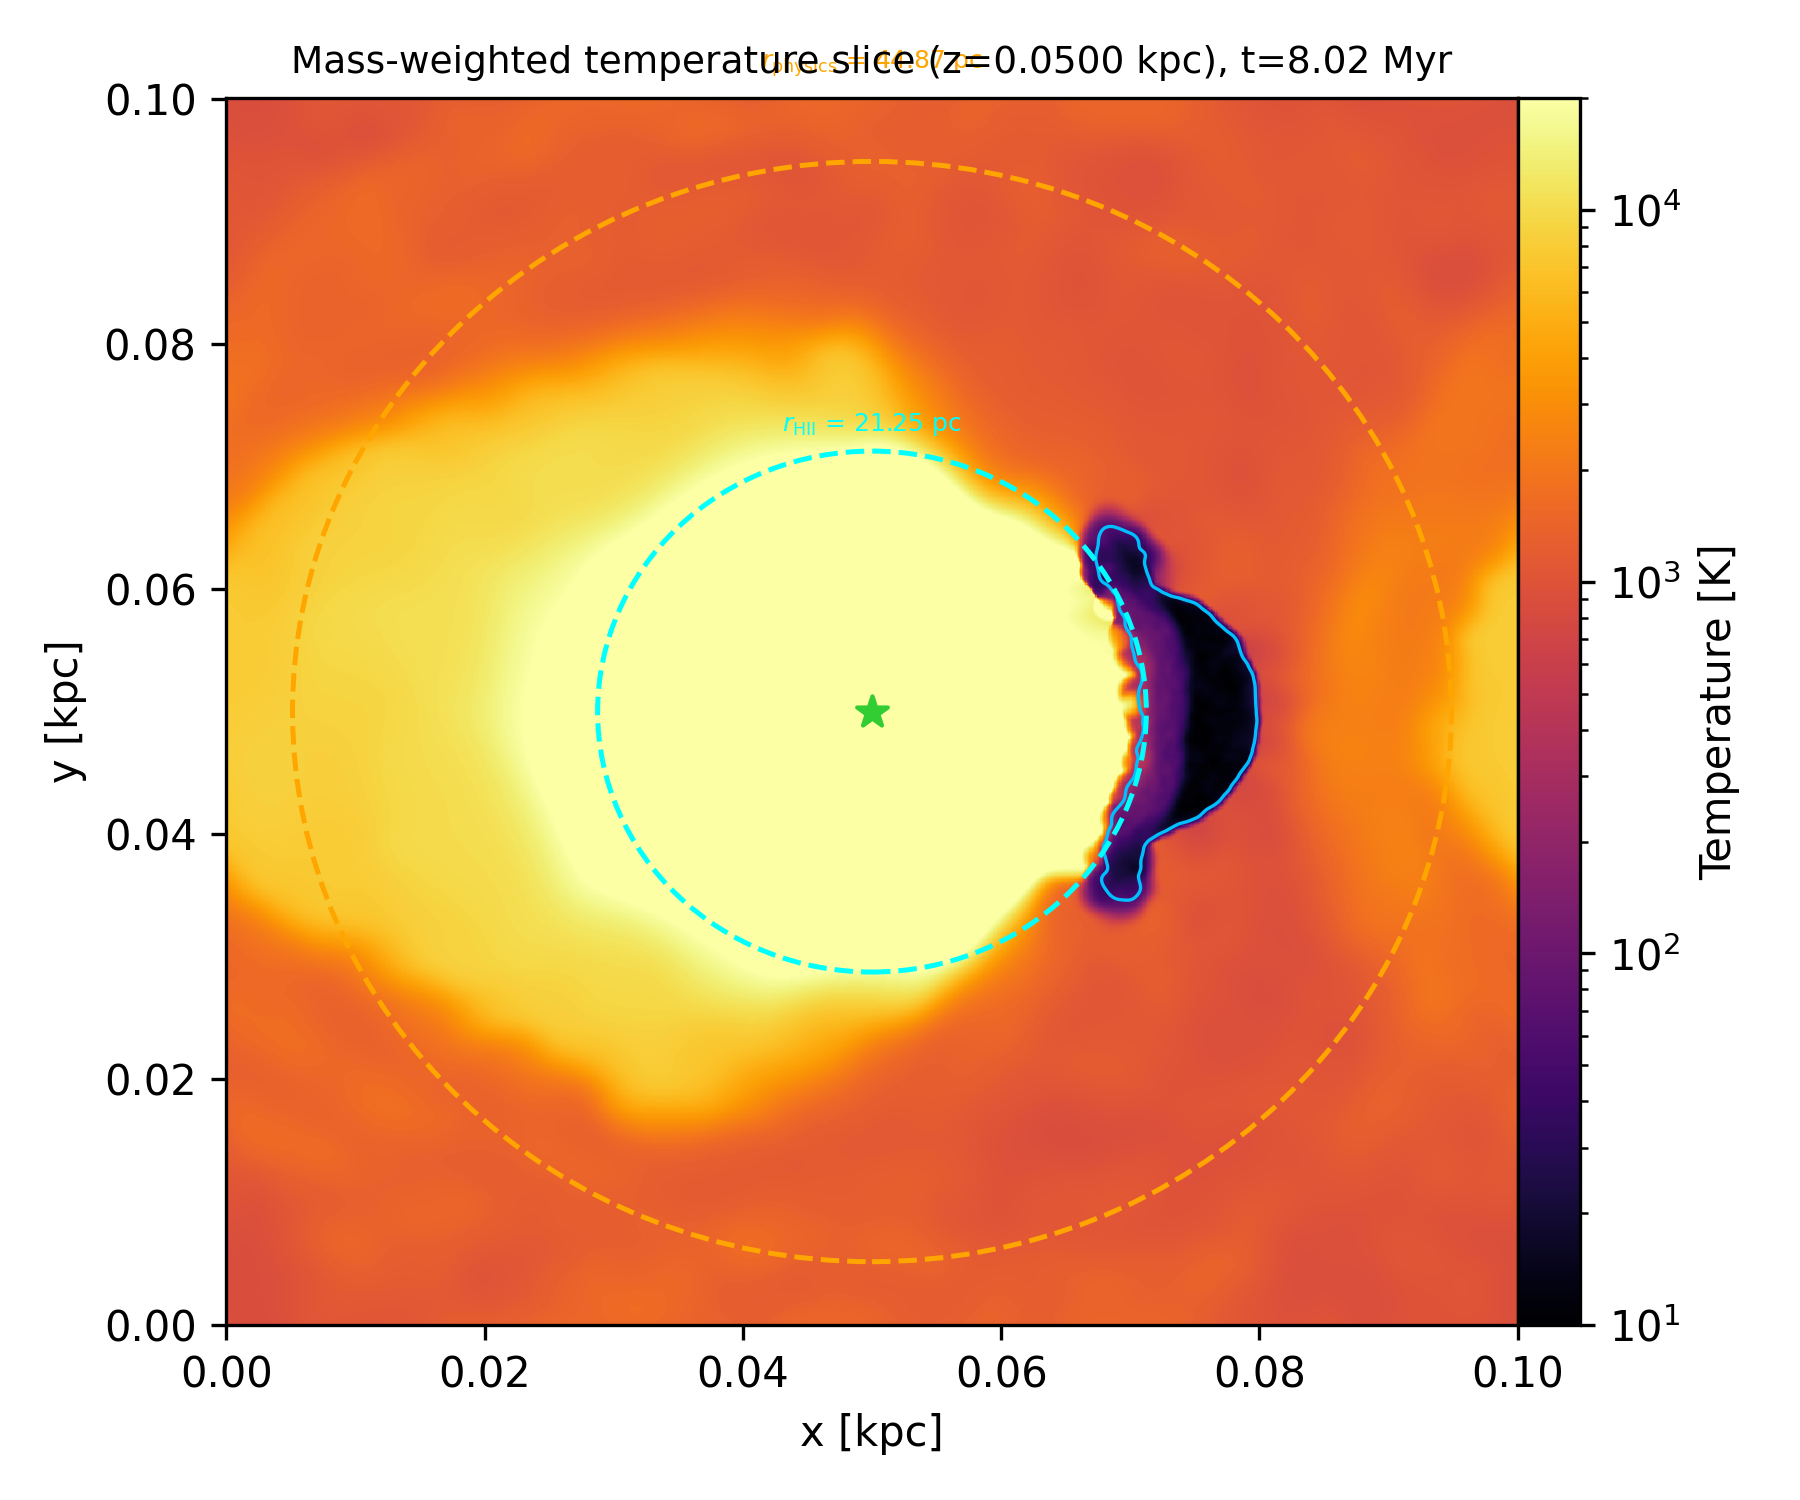
\includegraphics[width=0.48\linewidth]{Figures/tslice_gas20z0_nside0_rebuild0p01}
  \caption{Same configuration (\texttt{gas\_mass=20}, uniform,
    rebuild=0.01\,Myr) at $Z/Z_\odot\approx0.231$ (left) and $Z=0$
    (right). Left: clean black background, $r_{\rm physics}$ and
    $r_{\rm HII}$ agree closely. Right: the whole box is warm,
    $r_{\rm physics}$ more than doubles $r_{\rm HII}$ -- see text.}
  \label{fig:z0-vs-z0231-slice}
\end{figure}

The same comparison for the \emph{angular} scheme
(Figure~\ref{fig:z0-vs-z0231-slice-angular}) shows the identical
pattern, and more sharply: at $Z/Z_\odot\approx0.231$, $r_{\rm
HII}=27.72\,$pc and $r_{\rm physics}=21.05\,$pc -- the algorithm
already over-reports itself relative to the physically-hot gas, the
known angular-scheme bookkeeping bias discussed in
Section~\ref{sec:matrix-gas20}. At $Z=0$, $r_{\rm HII}=45.00\,$pc (the
search-radius cap) and $r_{\rm physics}=42.38\,$pc: both diagnostics
saturate near the cap, and the background-glow contamination is, if
anything, harder to disentangle from the bookkeeping bias here than in
the uniform case, since both push $r_{\rm physics}$ upward for
different reasons at once. This reinforces
Section~\ref{sec:matrix-gas20}'s point that the angular scheme's own
$r_{\rm HII}$ is already an unreliable size estimate independent of
metallicity; at $Z=0$ the two independent sources of overestimate
(angular bookkeeping bias and cooling-contaminated $r_{\rm physics}$)
compound rather than cancel.

\begin{figure}
  \centering
  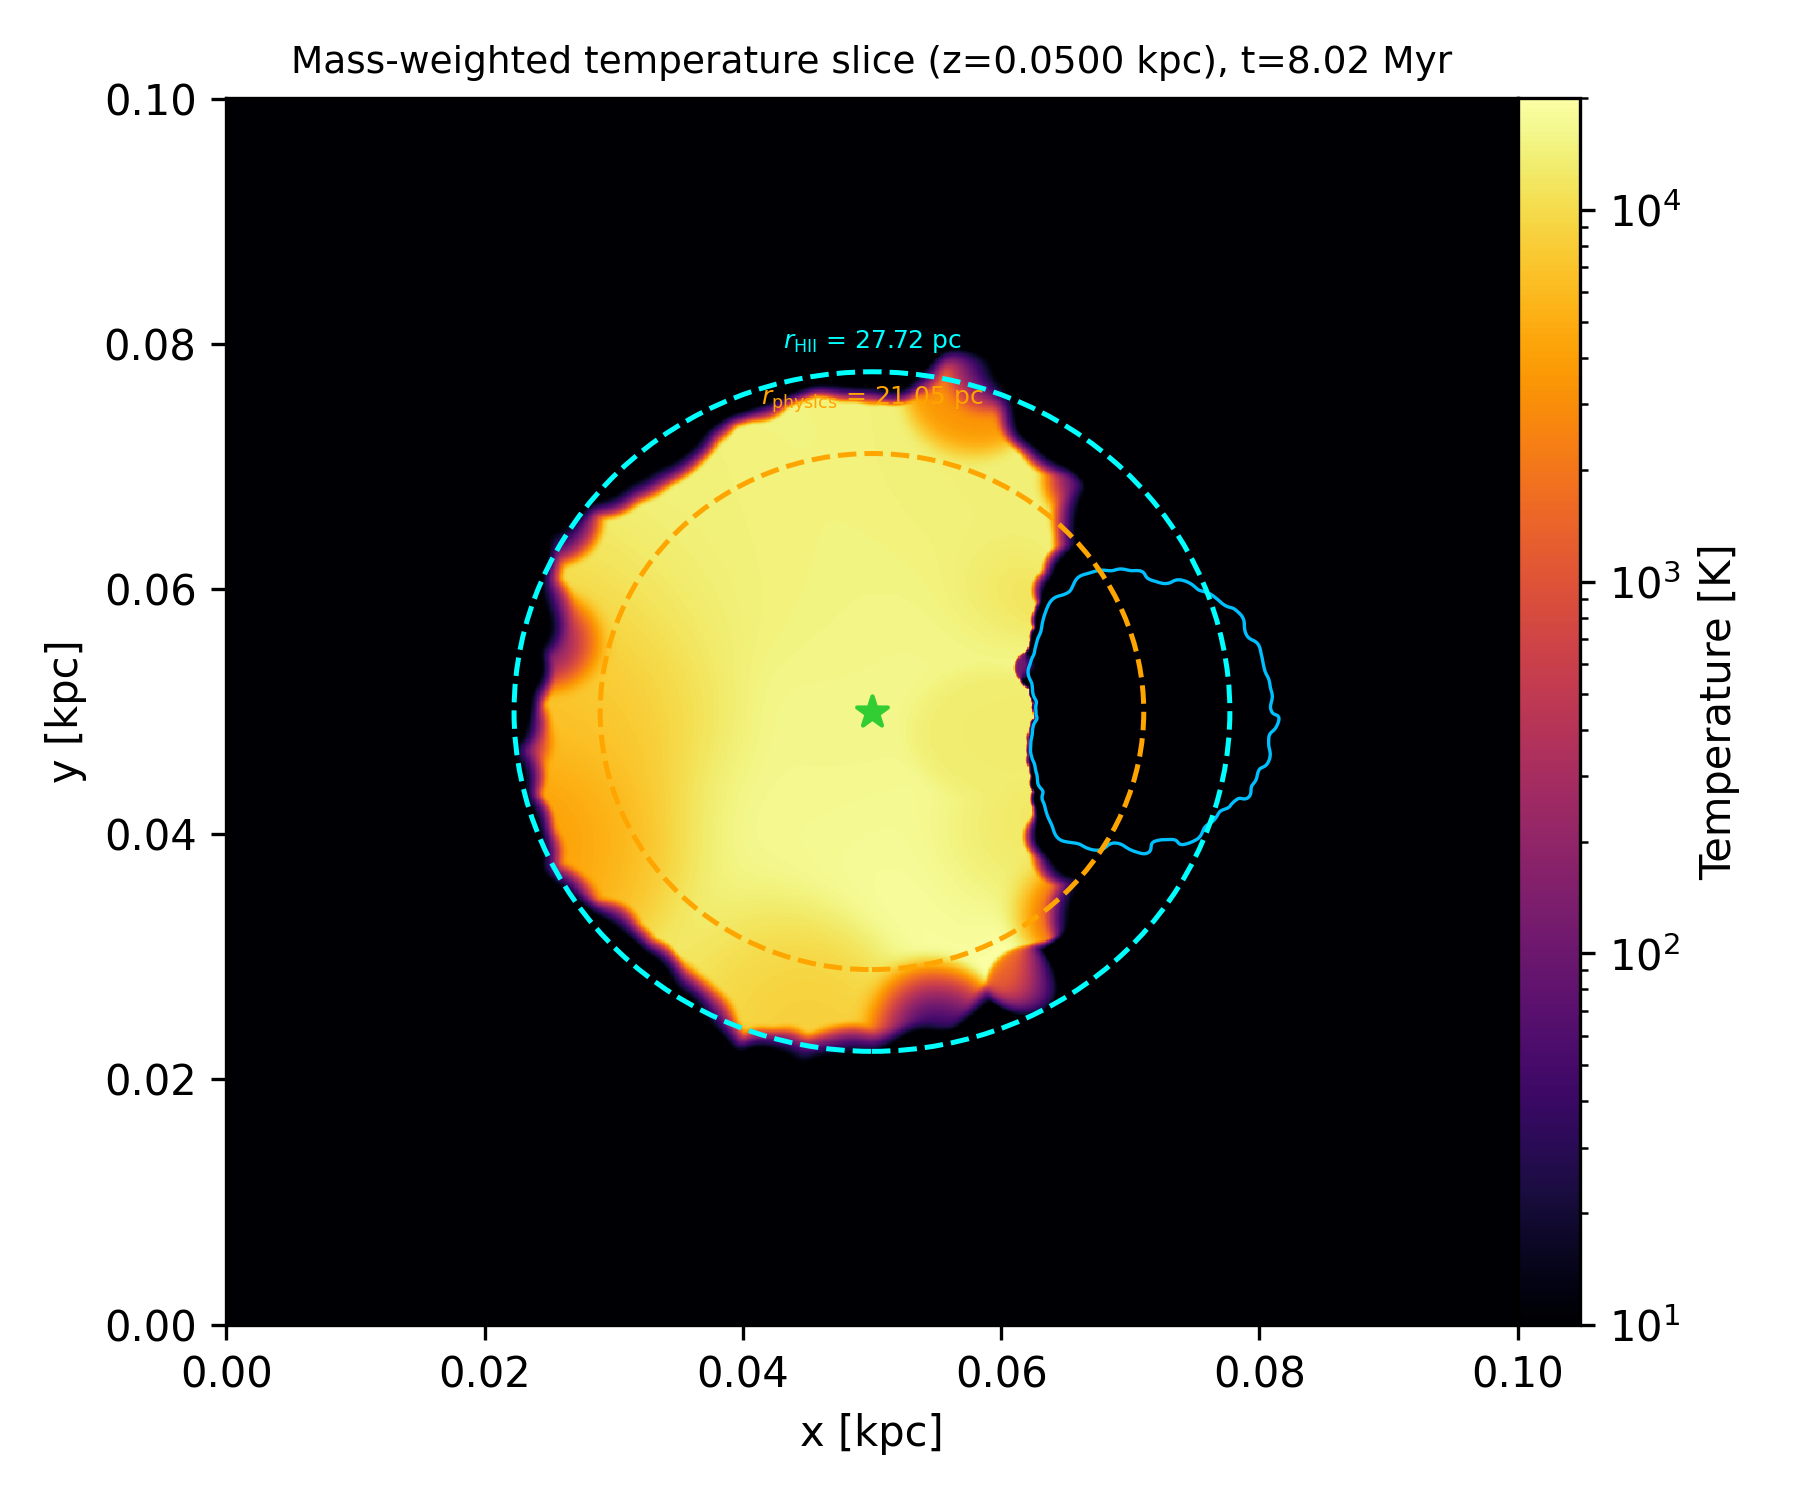
\includegraphics[width=0.48\linewidth]{Figures/tslice_gas20_nside1_rebuild0p01}
  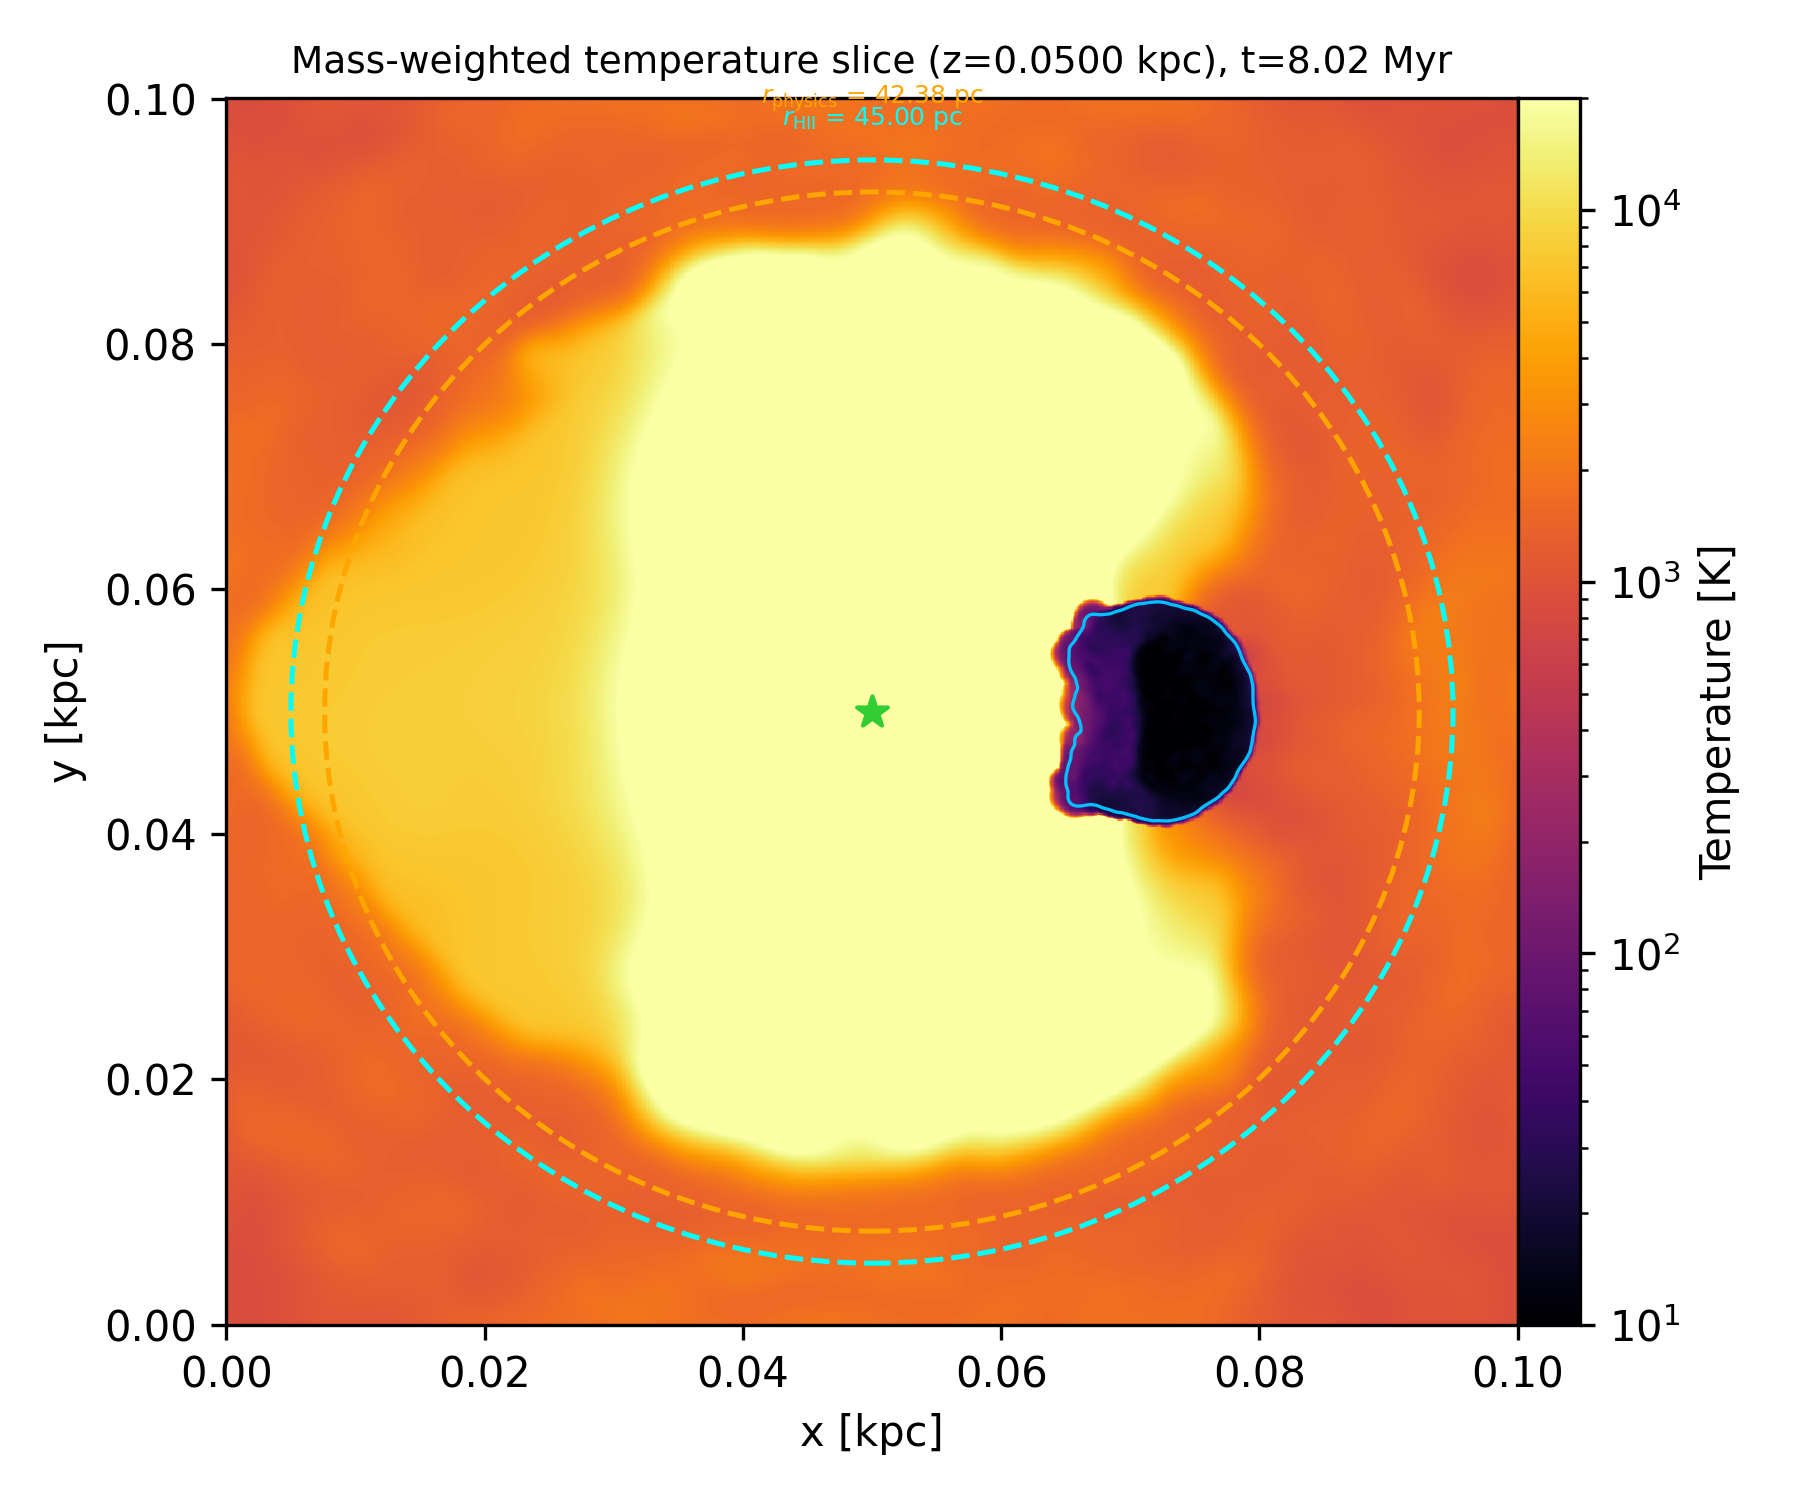
\includegraphics[width=0.48\linewidth]{Figures/tslice_gas20z0_nside1_rebuild0p01}
  \caption{Same comparison as Figure~\ref{fig:z0-vs-z0231-slice}, but
    for the \emph{angular} scheme (\texttt{gas\_mass=20}, nside=1,
    rebuild=0.01\,Myr): $Z/Z_\odot\approx0.231$ (left,
    $r_{\rm HII}=27.72\,$pc, $r_{\rm physics}=21.05\,$pc) versus $Z=0$
    (right, $r_{\rm HII}=45.00\,$pc -- the search-radius cap,
    $r_{\rm physics}=42.38\,$pc).}
  \label{fig:z0-vs-z0231-slice-angular}
\end{figure}

\begin{figure}
  \centering
  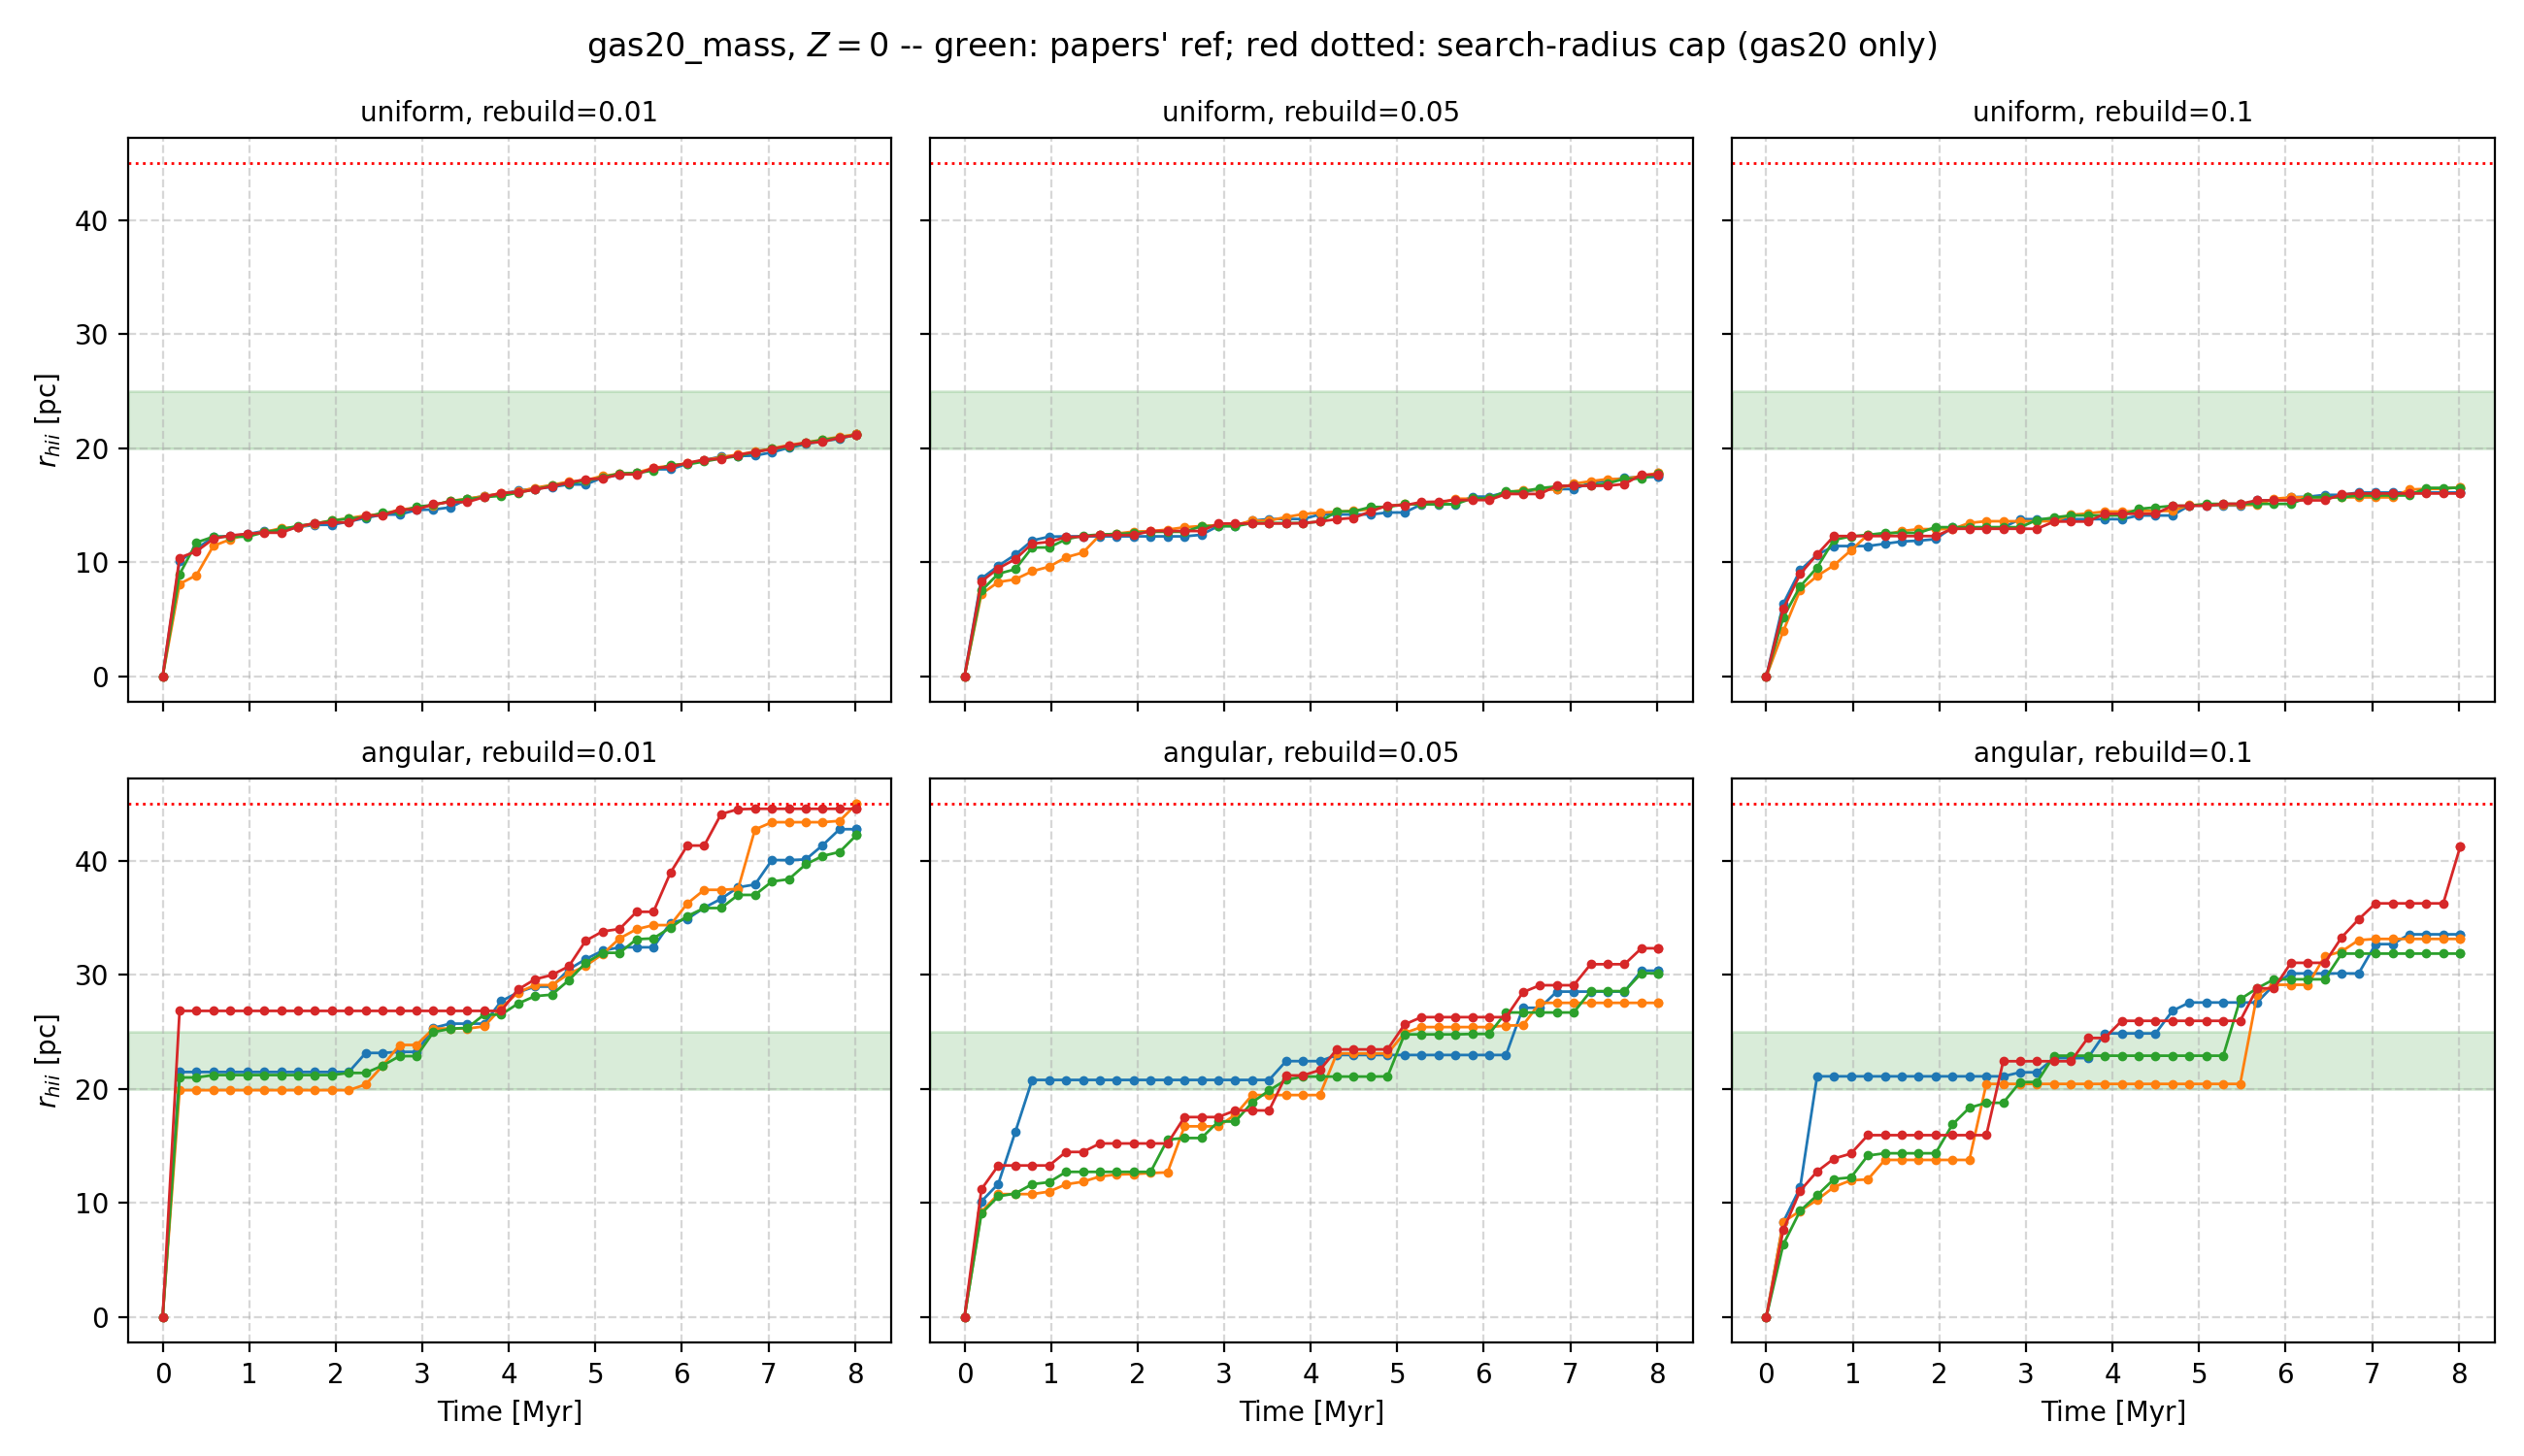
\includegraphics[width=\linewidth]{Figures/gas20_z0_matrix}
  \caption{Per-star $r_{\rm HII}(t)$ at \texttt{gas\_mass=20}, $Z=0$,
    for all six configurations. Green band: the papers' reference.
    Red dotted line: the 45\,pc search-radius cap -- angular,
    rebuild=0.01\,Myr (bottom left) runs into it, as expected without
    widening.}
  \label{fig:gas20-z0-growth}
\end{figure}

\begin{figure}
  \centering
  \begin{tabular}{@{}c@{}c@{}c@{}}
    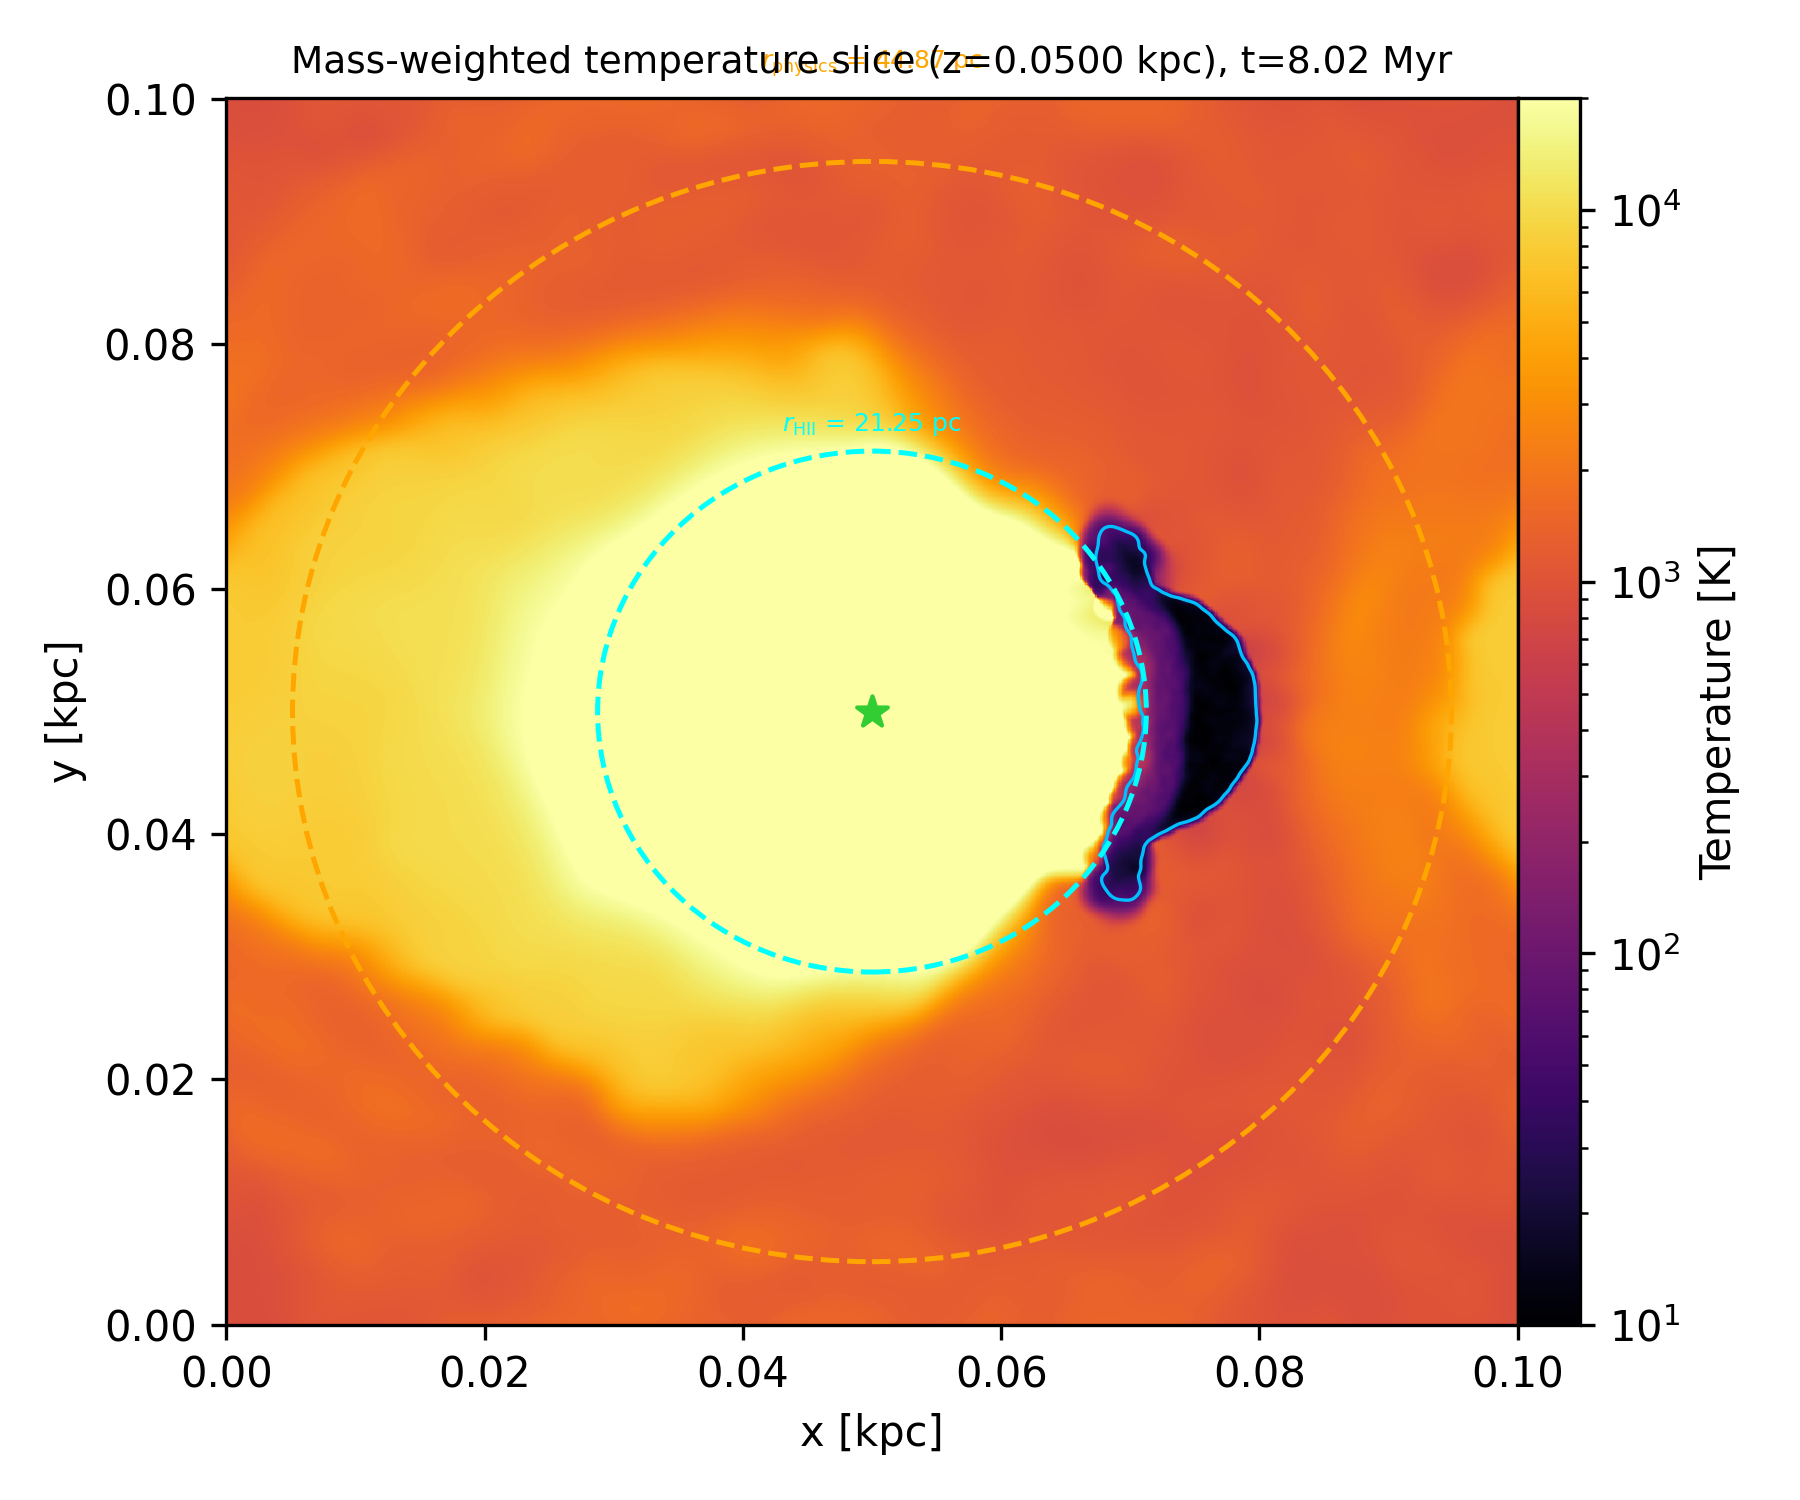
\includegraphics[width=0.325\linewidth]{Figures/tslice_gas20z0_nside0_rebuild0p01} &
    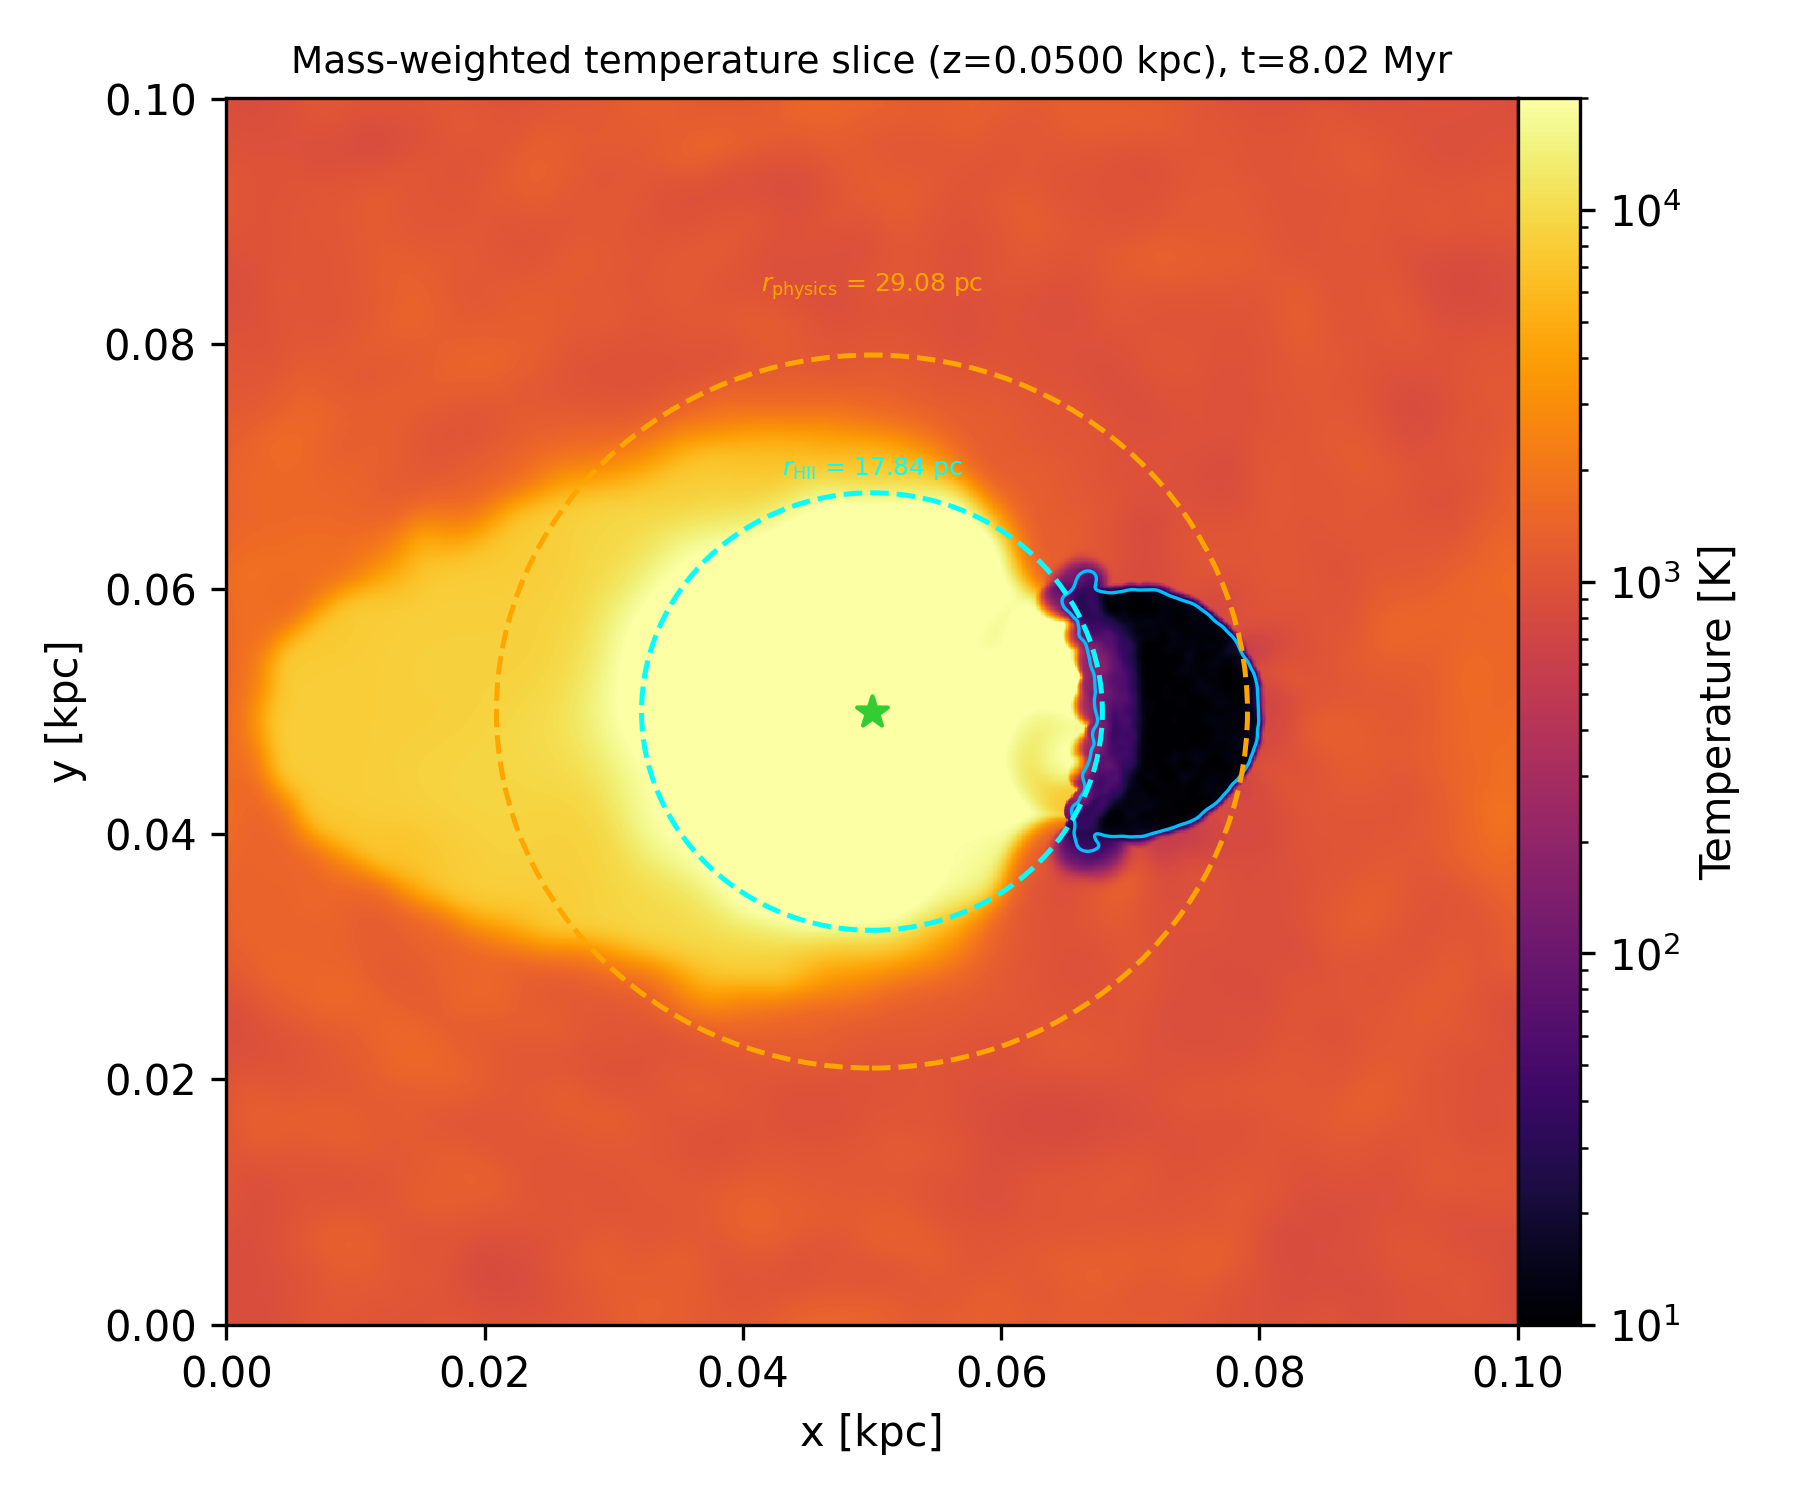
\includegraphics[width=0.325\linewidth]{Figures/tslice_gas20z0_nside0_rebuild0p05} &
    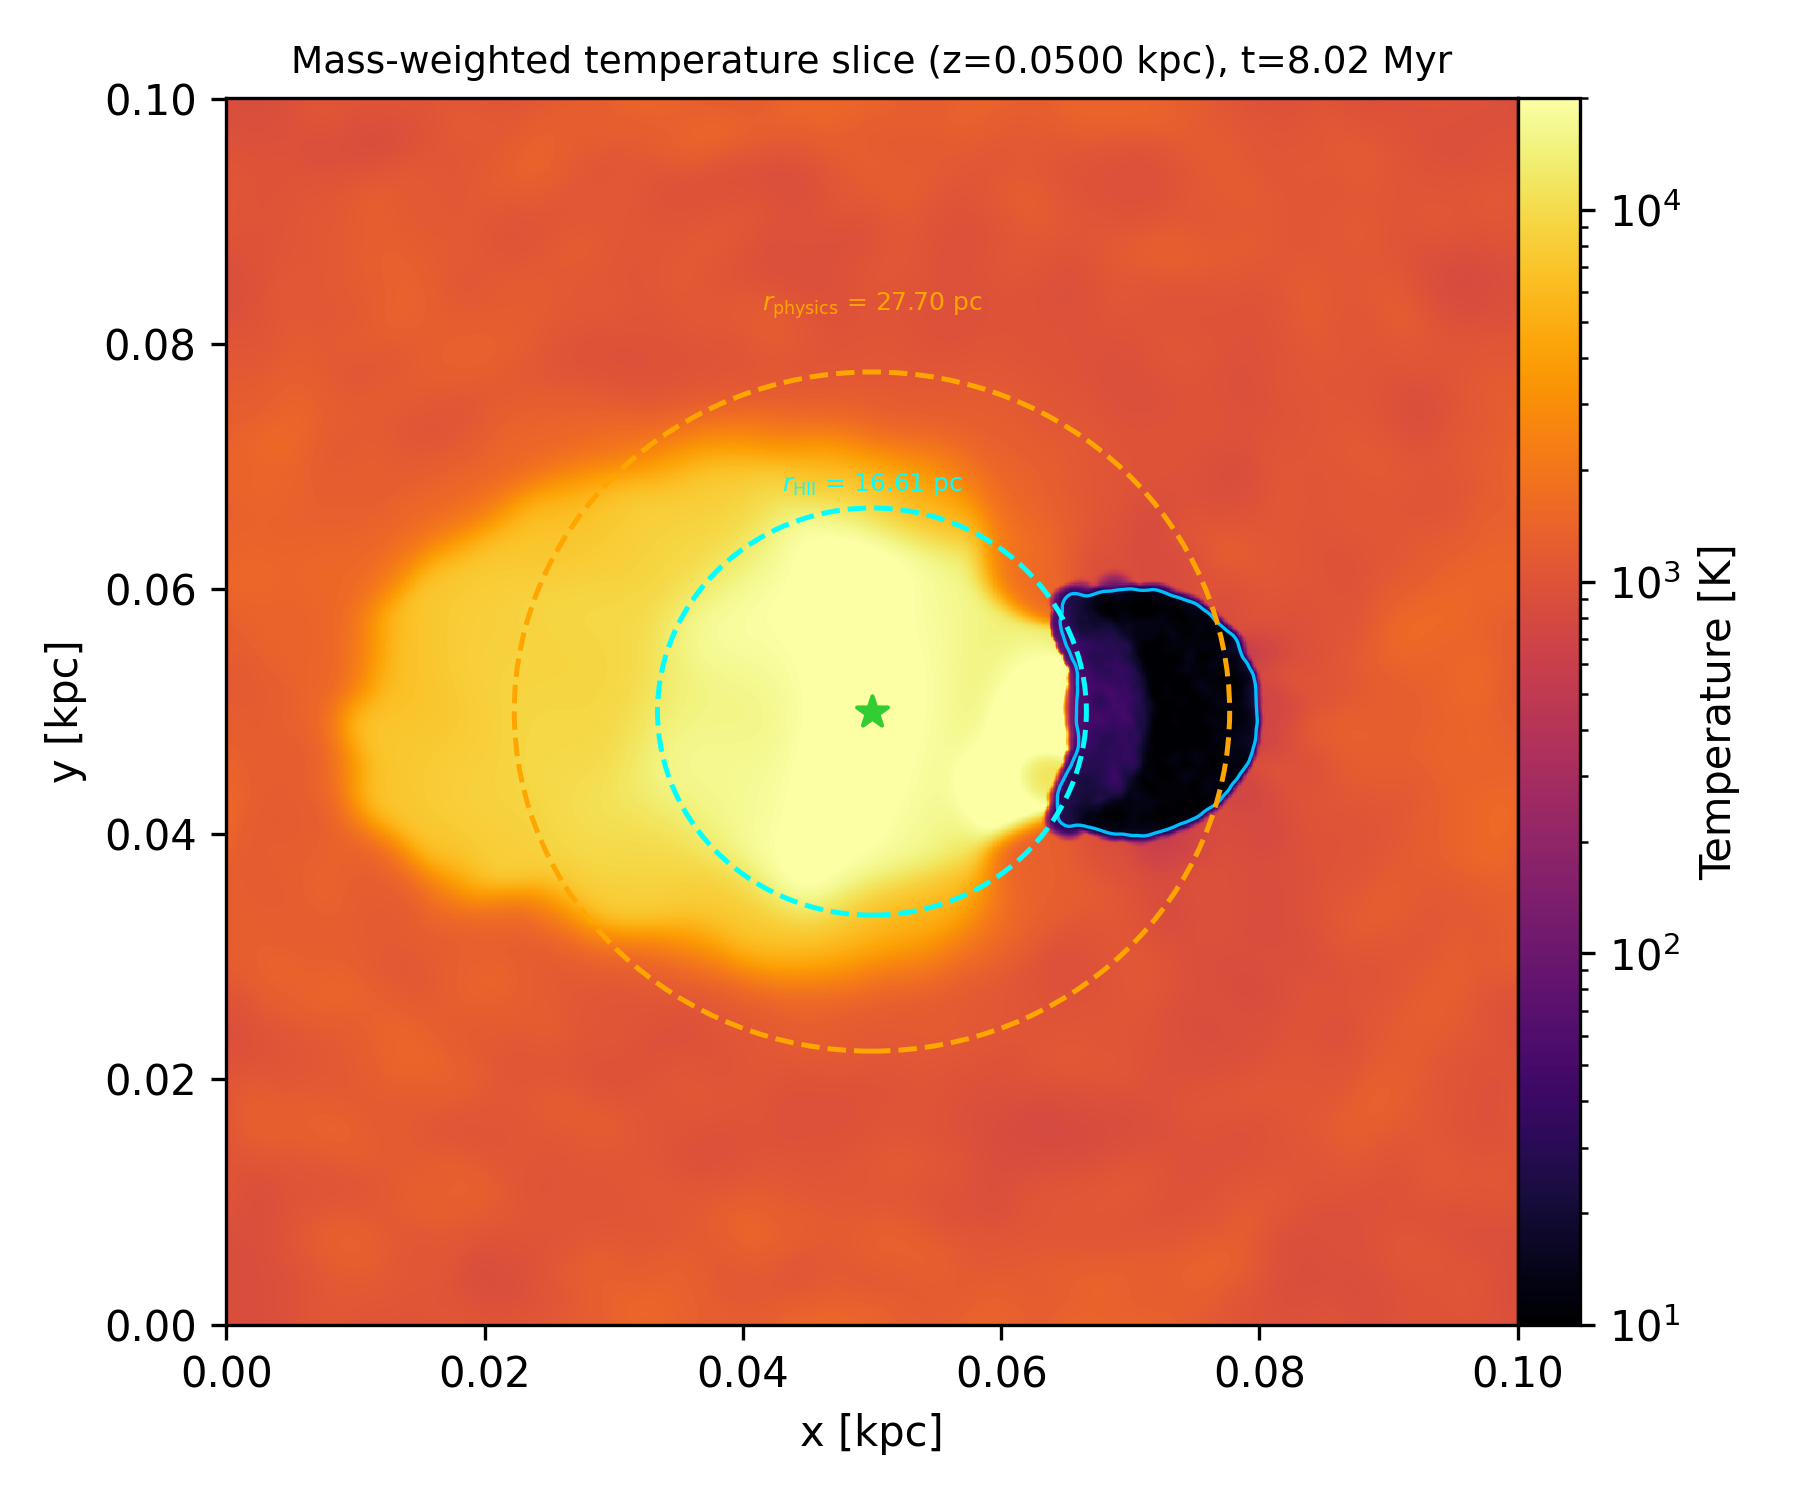
\includegraphics[width=0.325\linewidth]{Figures/tslice_gas20z0_nside0_rebuild0p1} \\
    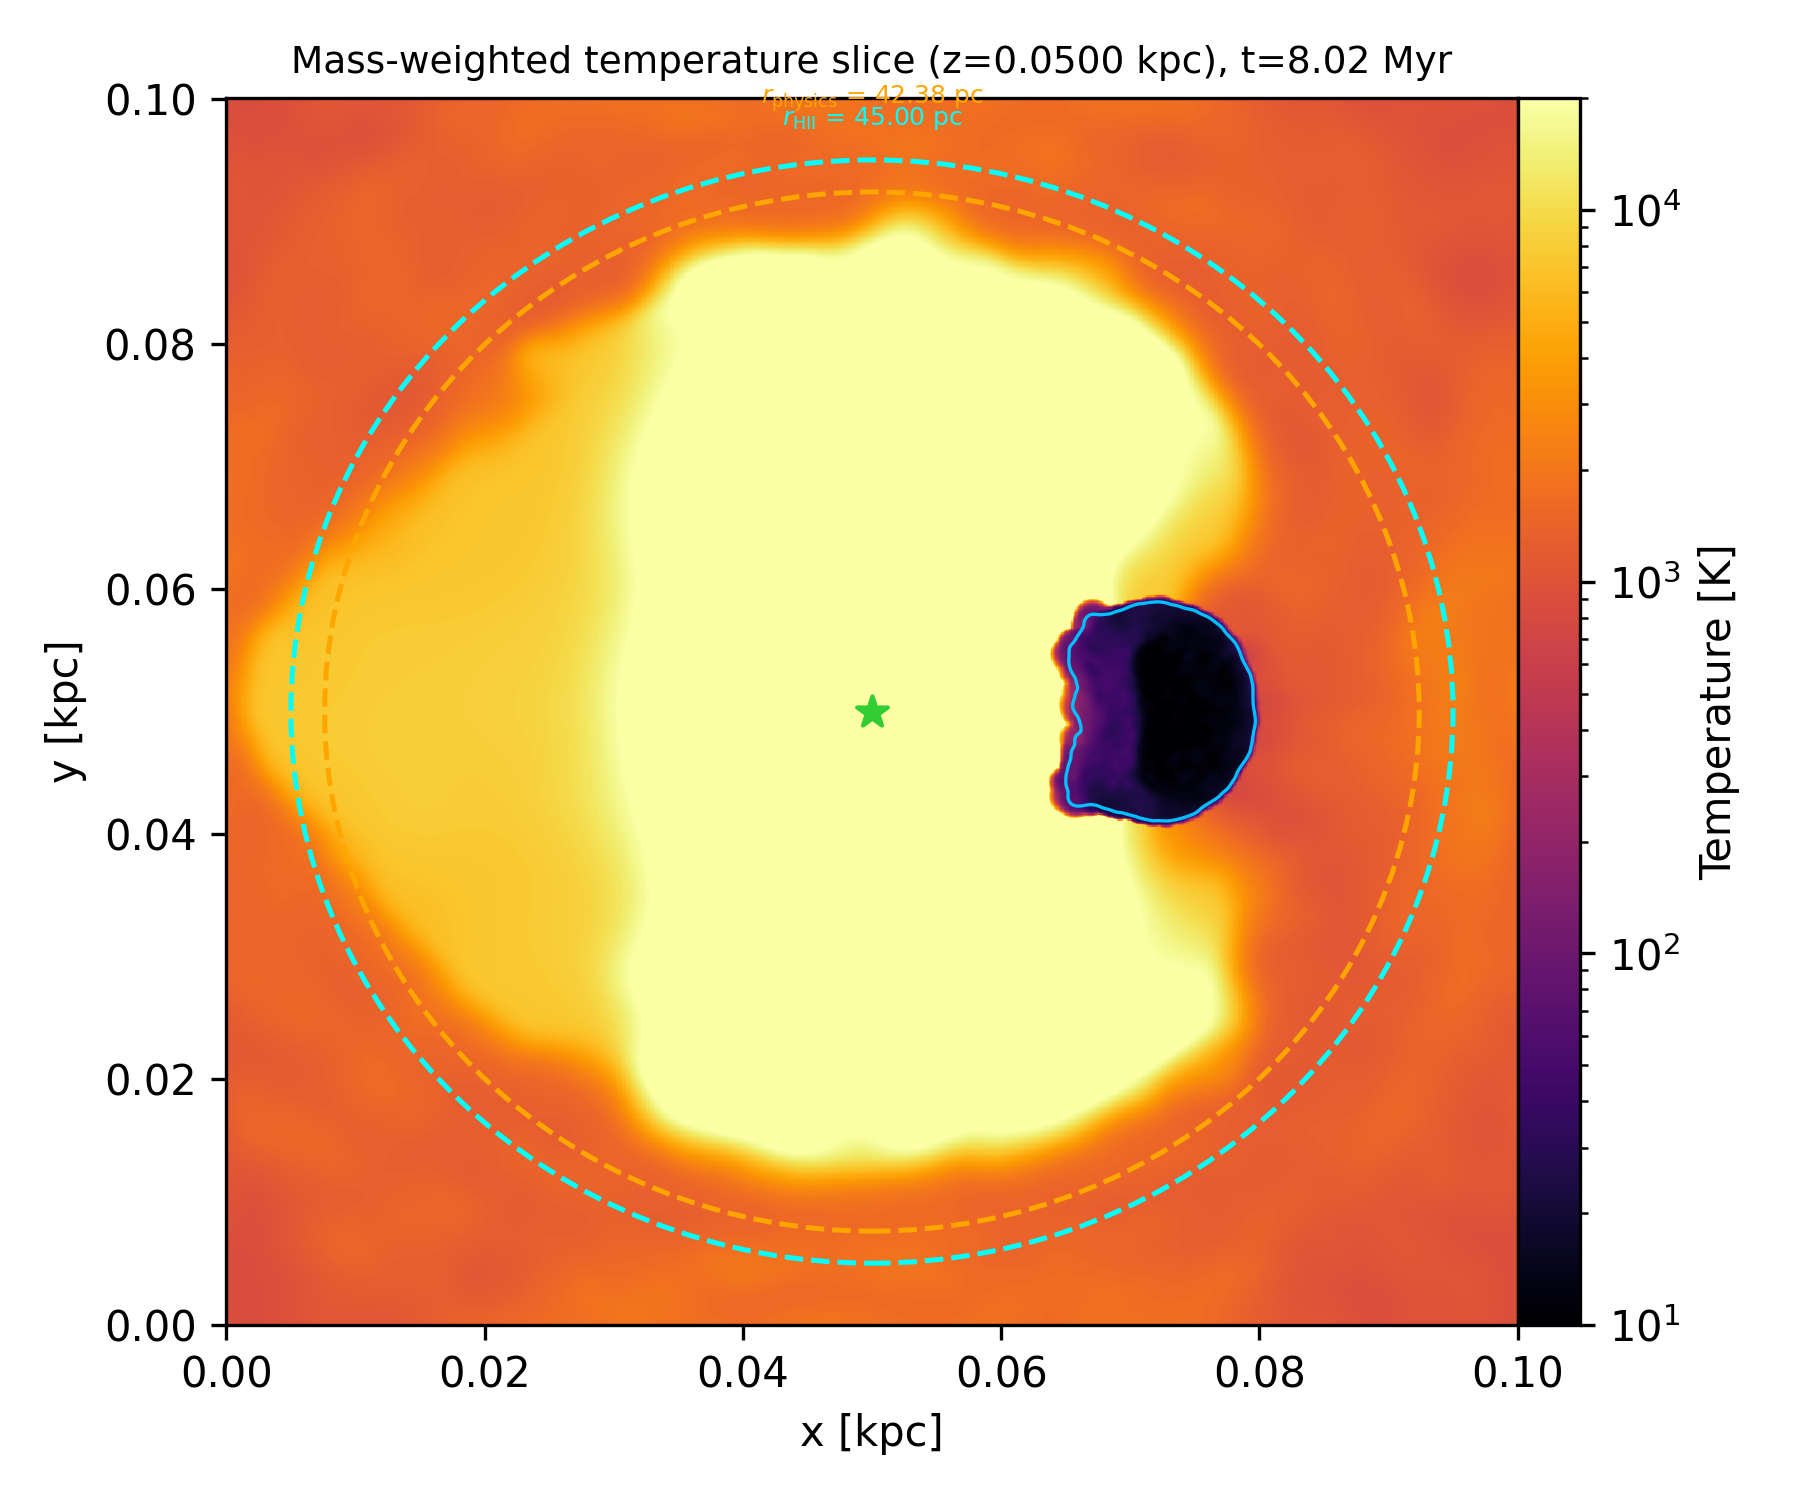
\includegraphics[width=0.325\linewidth]{Figures/tslice_gas20z0_nside1_rebuild0p01} &
    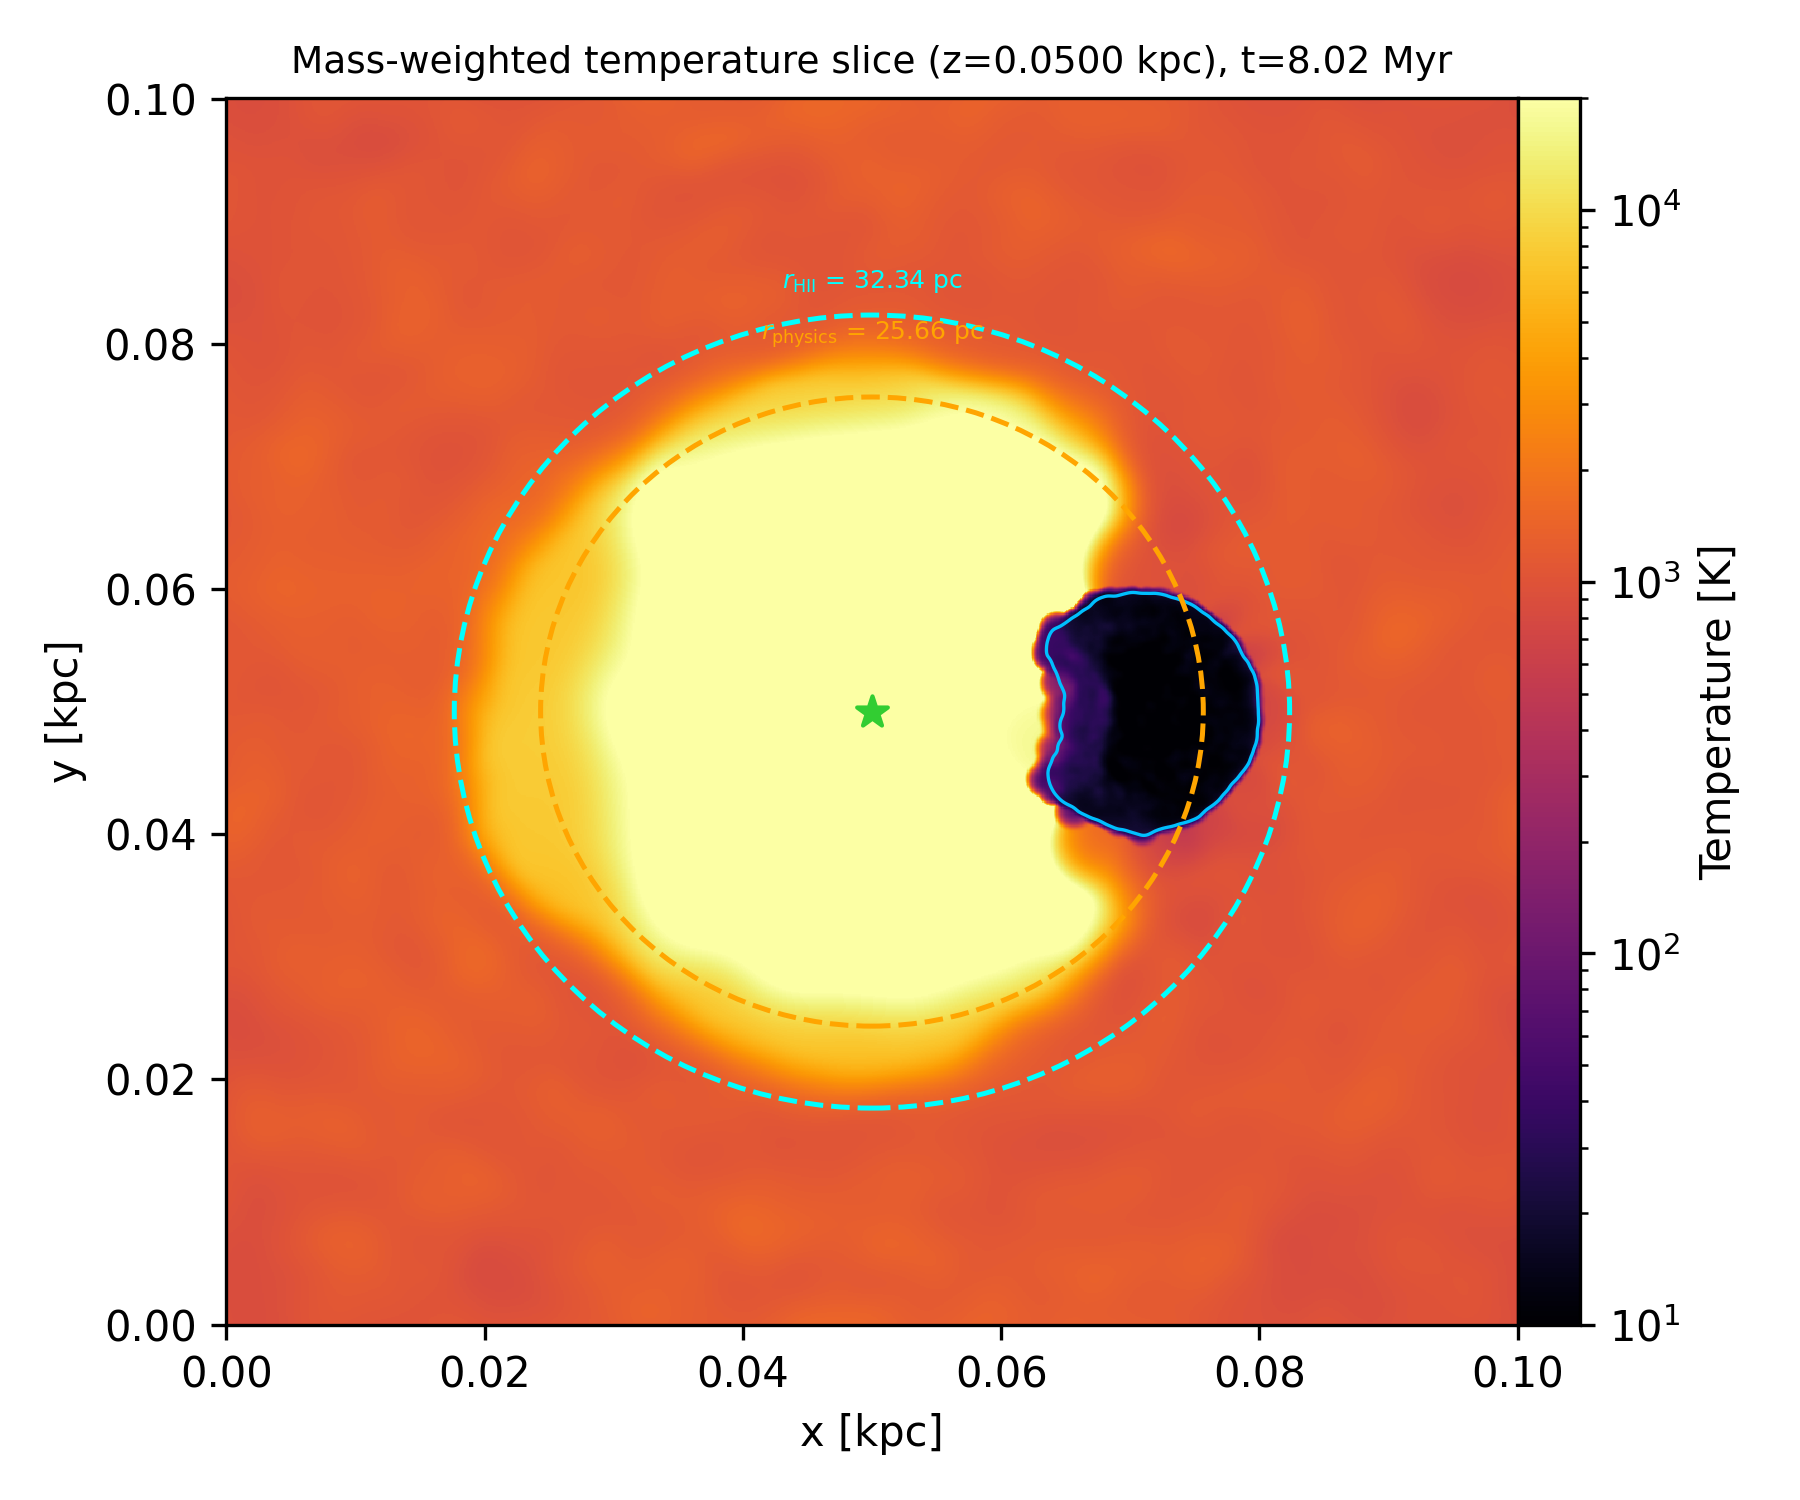
\includegraphics[width=0.325\linewidth]{Figures/tslice_gas20z0_nside1_rebuild0p05} &
    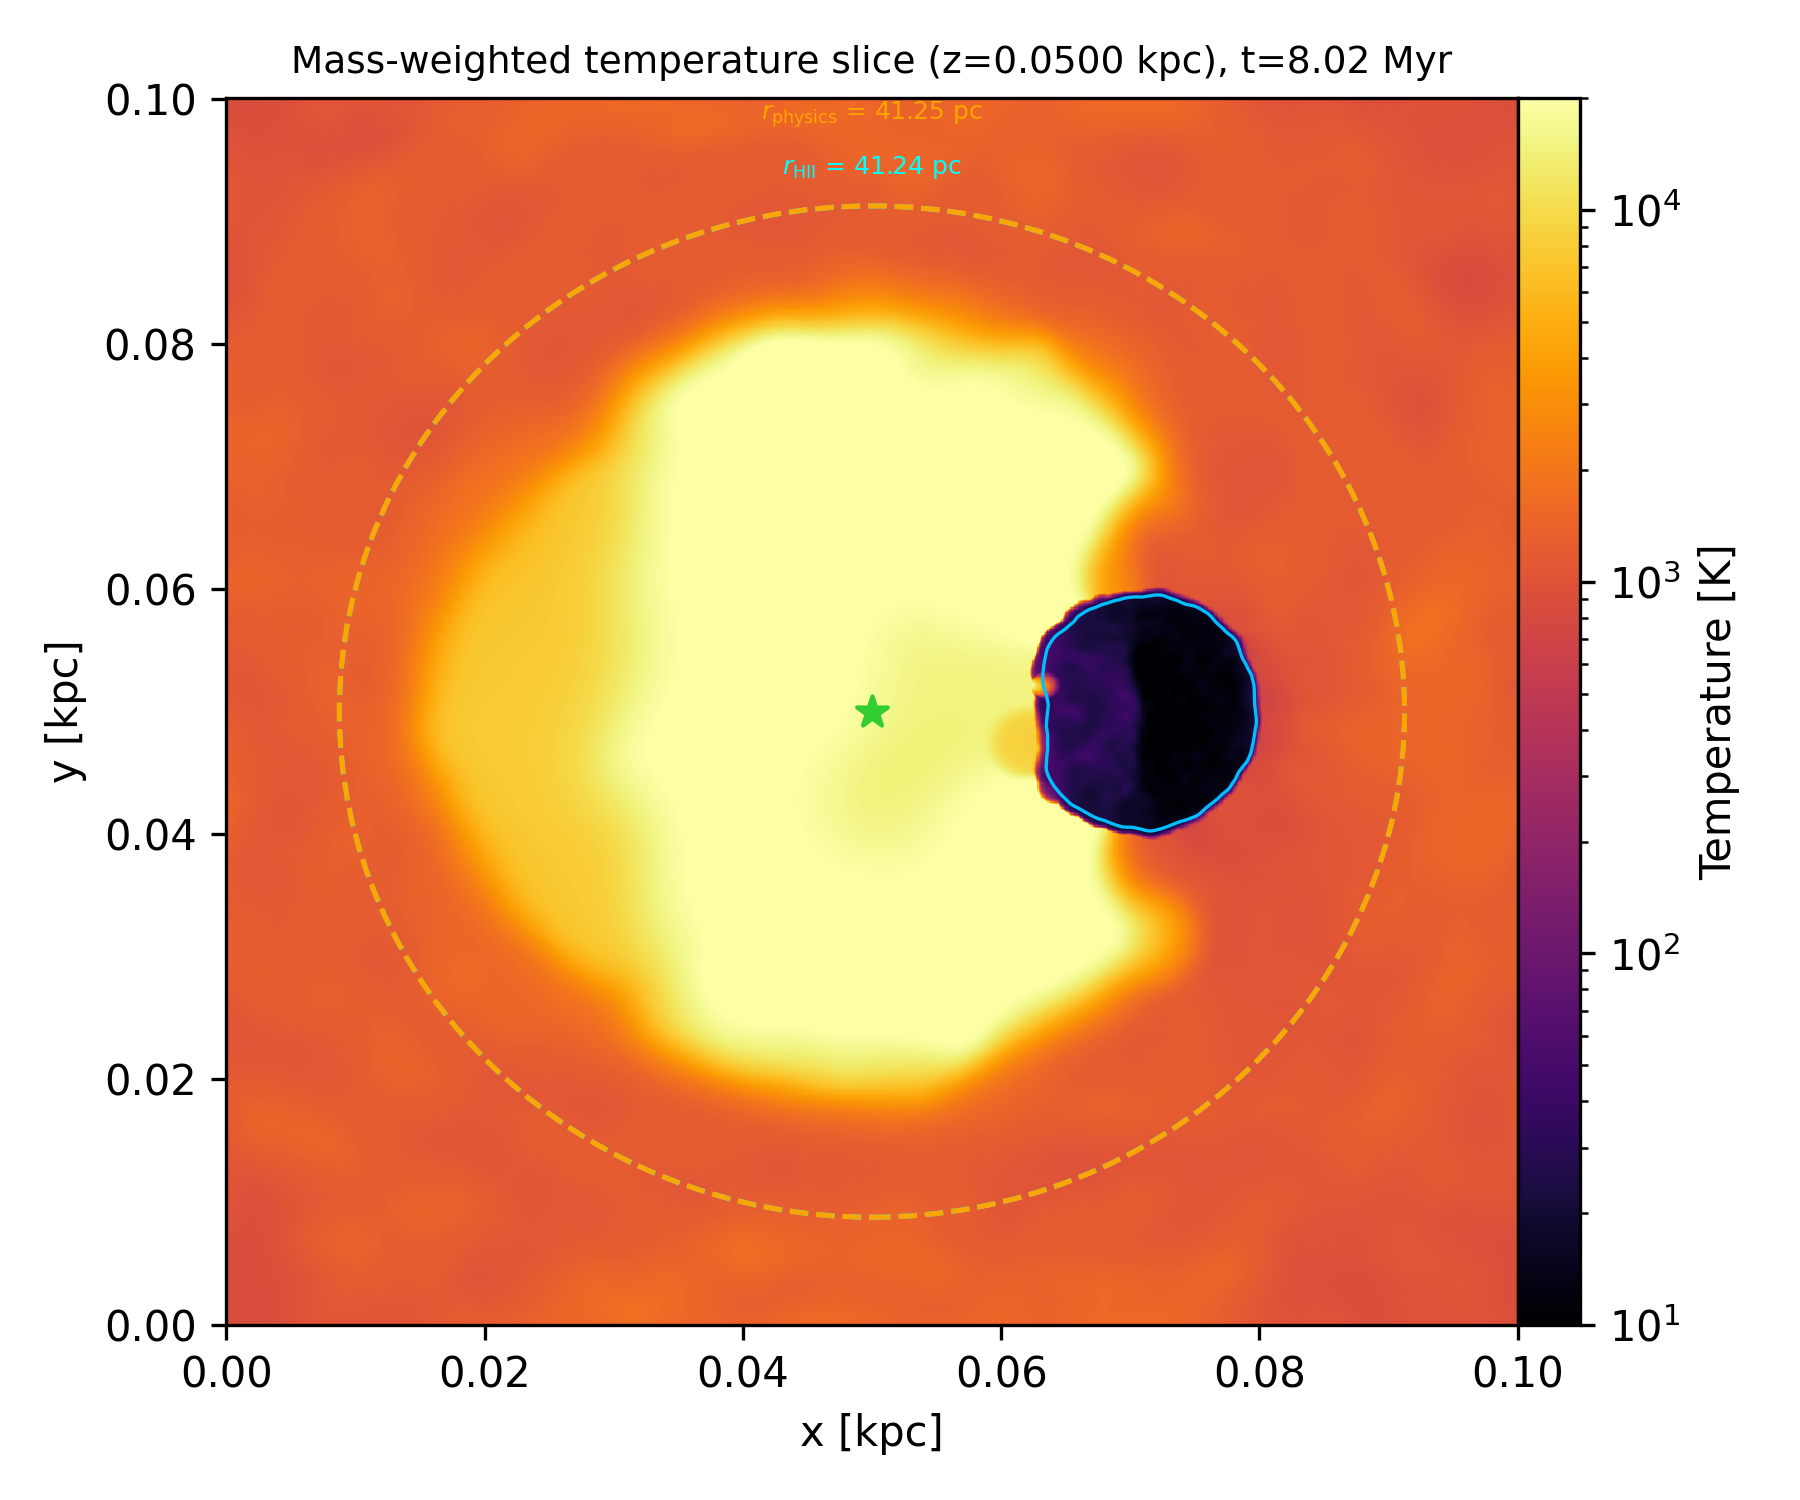
\includegraphics[width=0.325\linewidth]{Figures/tslice_gas20z0_nside1_rebuild0p1} \\
  \end{tabular}
  \caption{Temperature slices at $t=8\,$Myr, \texttt{gas\_mass=20},
    $Z=0$. Top row: uniform (nside=0), rebuild$\in\{0.01,0.05,0.1\}$\,Myr
    left to right. Bottom row: angular (nside=1), same rebuild order.
    Cyan circle: $r_{\rm HII}$. Orange circle: $r_{\rm physics}$. Blue
    contour: the clump's $n_H=1000\,{\rm cm^{-3}}$ density boundary.
    Compare against Figure~\ref{fig:gas20-slices}: the warm background
    glow visible in every panel here (versus clean black there) is the
    $r_{\rm physics}$-contamination effect discussed in the text, and
    makes the clump erosion pattern harder to read cleanly than at
    $Z/Z_\odot\approx0.231$.}
  \label{fig:gas20-z0-slices}
\end{figure}

\begin{figure}
  \centering
  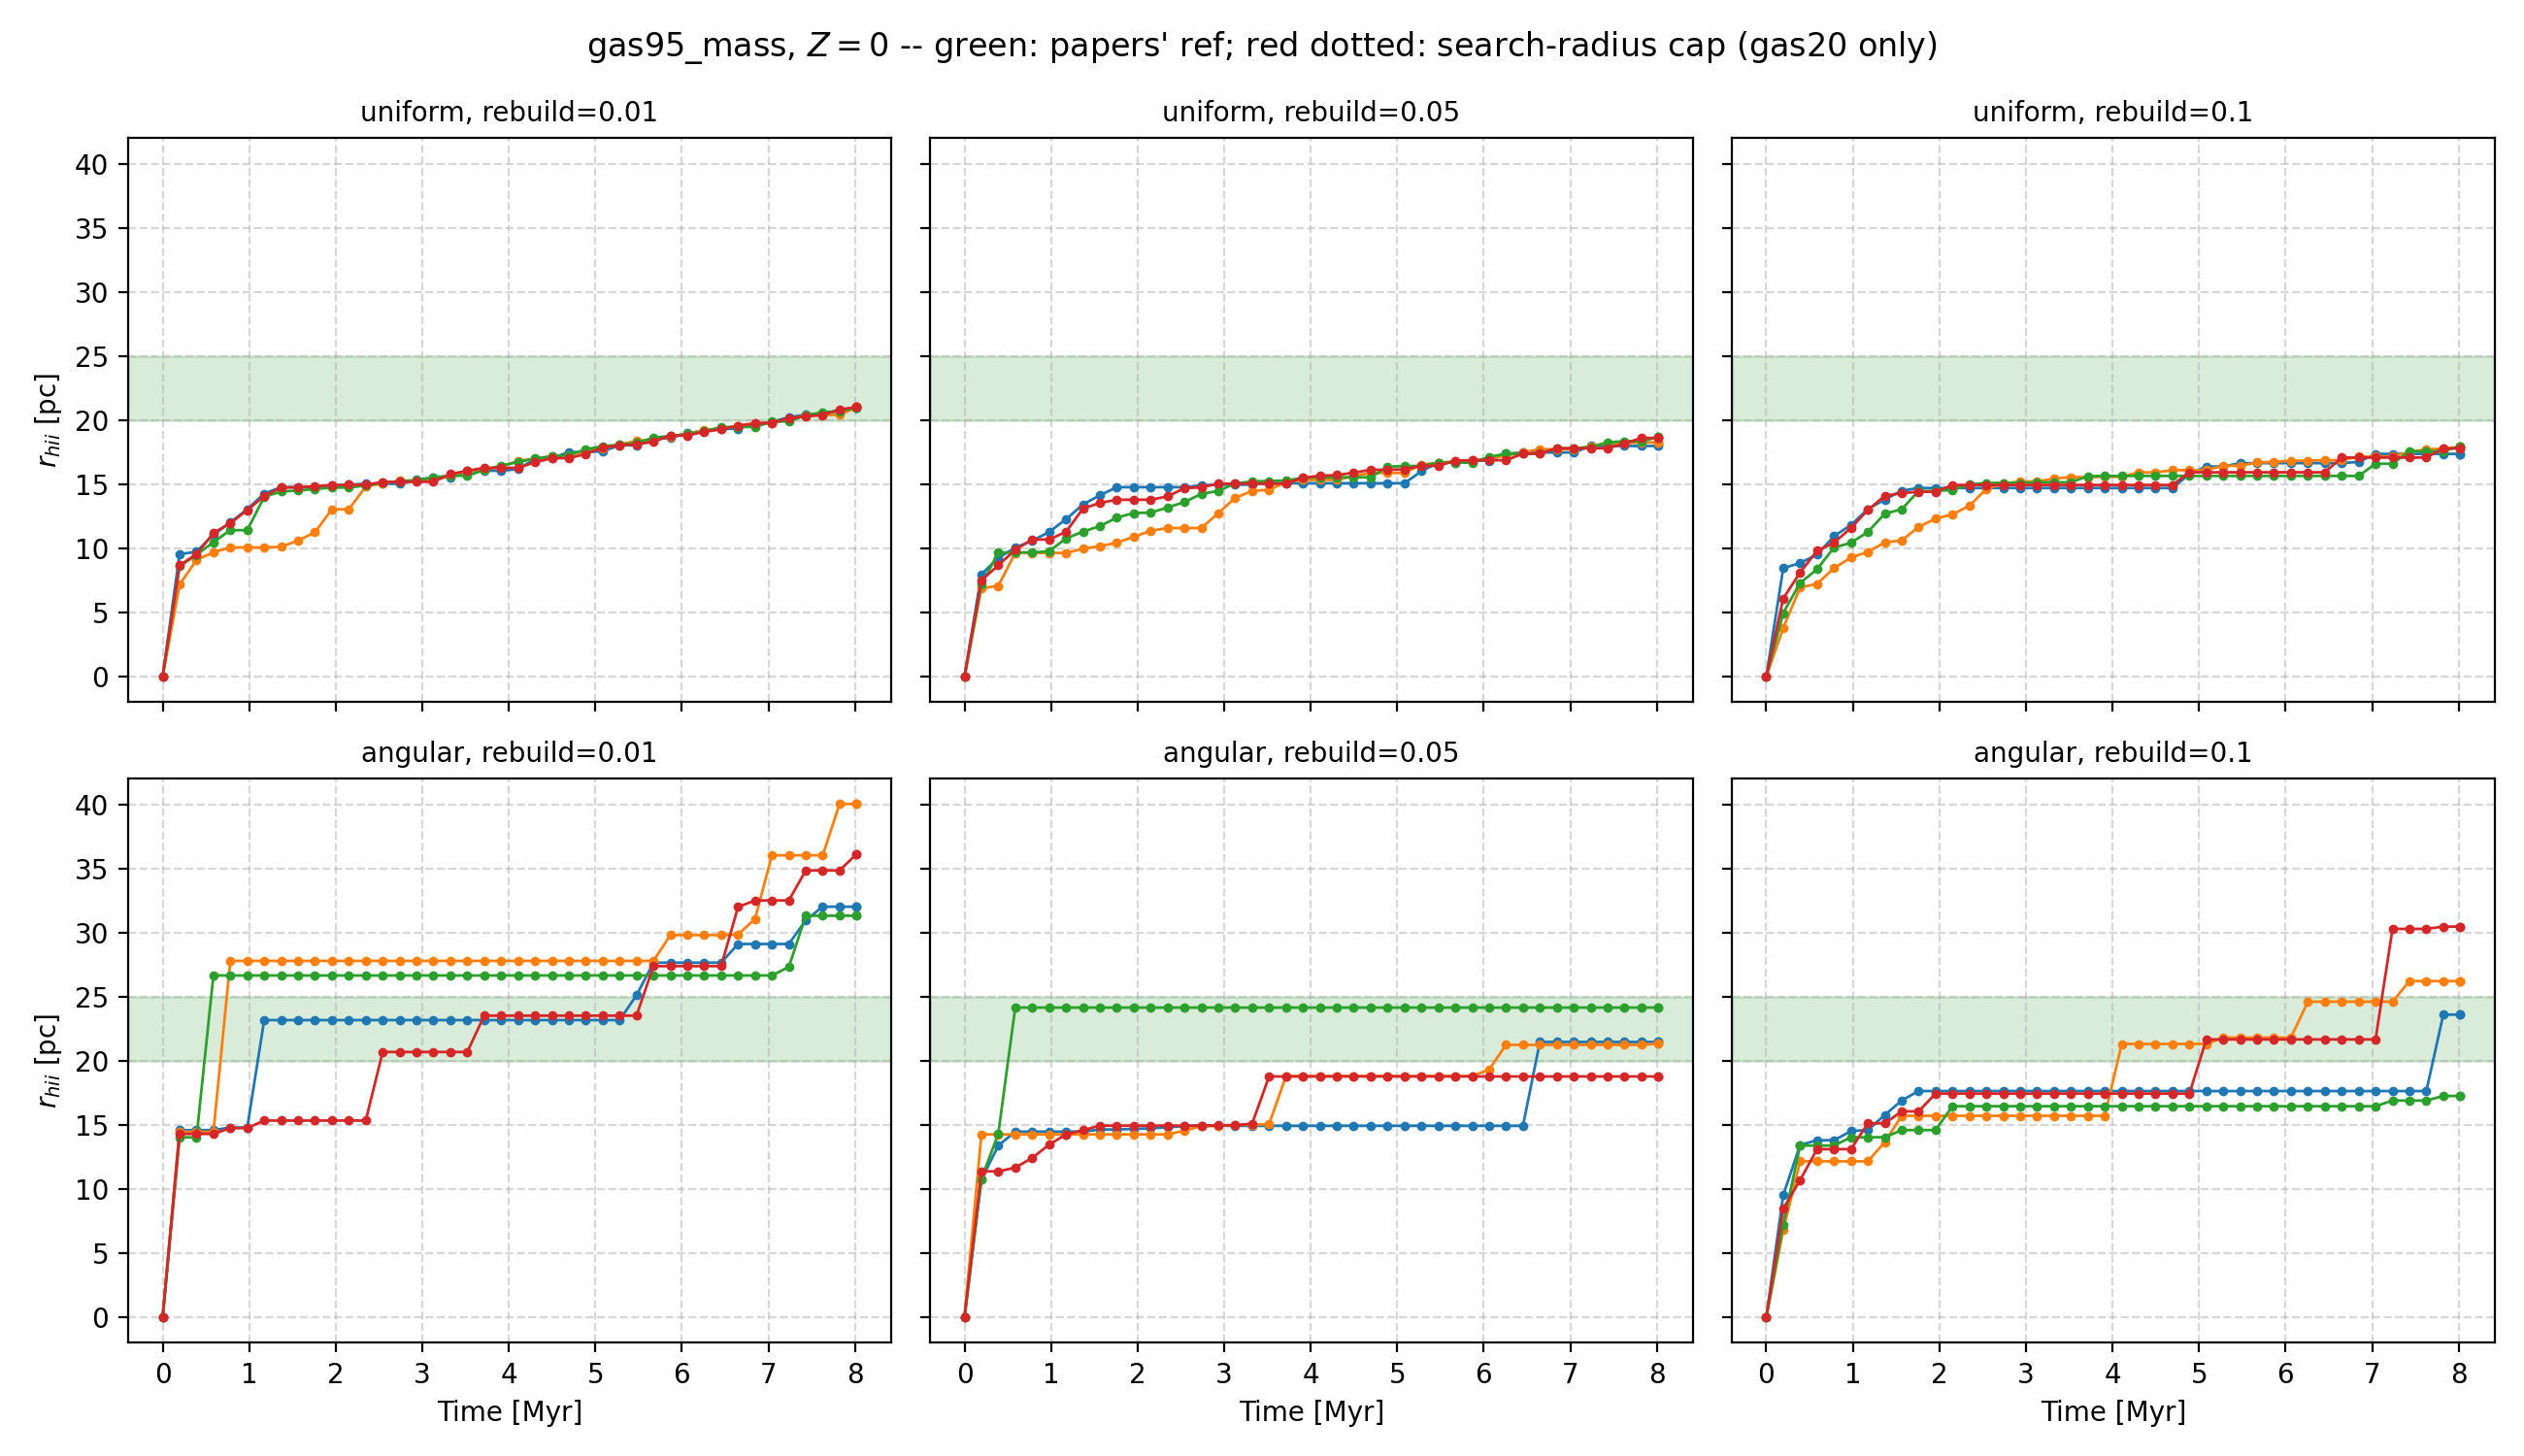
\includegraphics[width=\linewidth]{Figures/gas95_z0_matrix}
  \caption{Per-star $r_{\rm HII}(t)$ at \texttt{gas\_mass=95}, $Z=0$,
    for all six configurations. Green band: the papers' reference.}
  \label{fig:gas95-z0-growth}
\end{figure}

\begin{figure}
  \centering
  \begin{tabular}{@{}c@{}c@{}c@{}}
    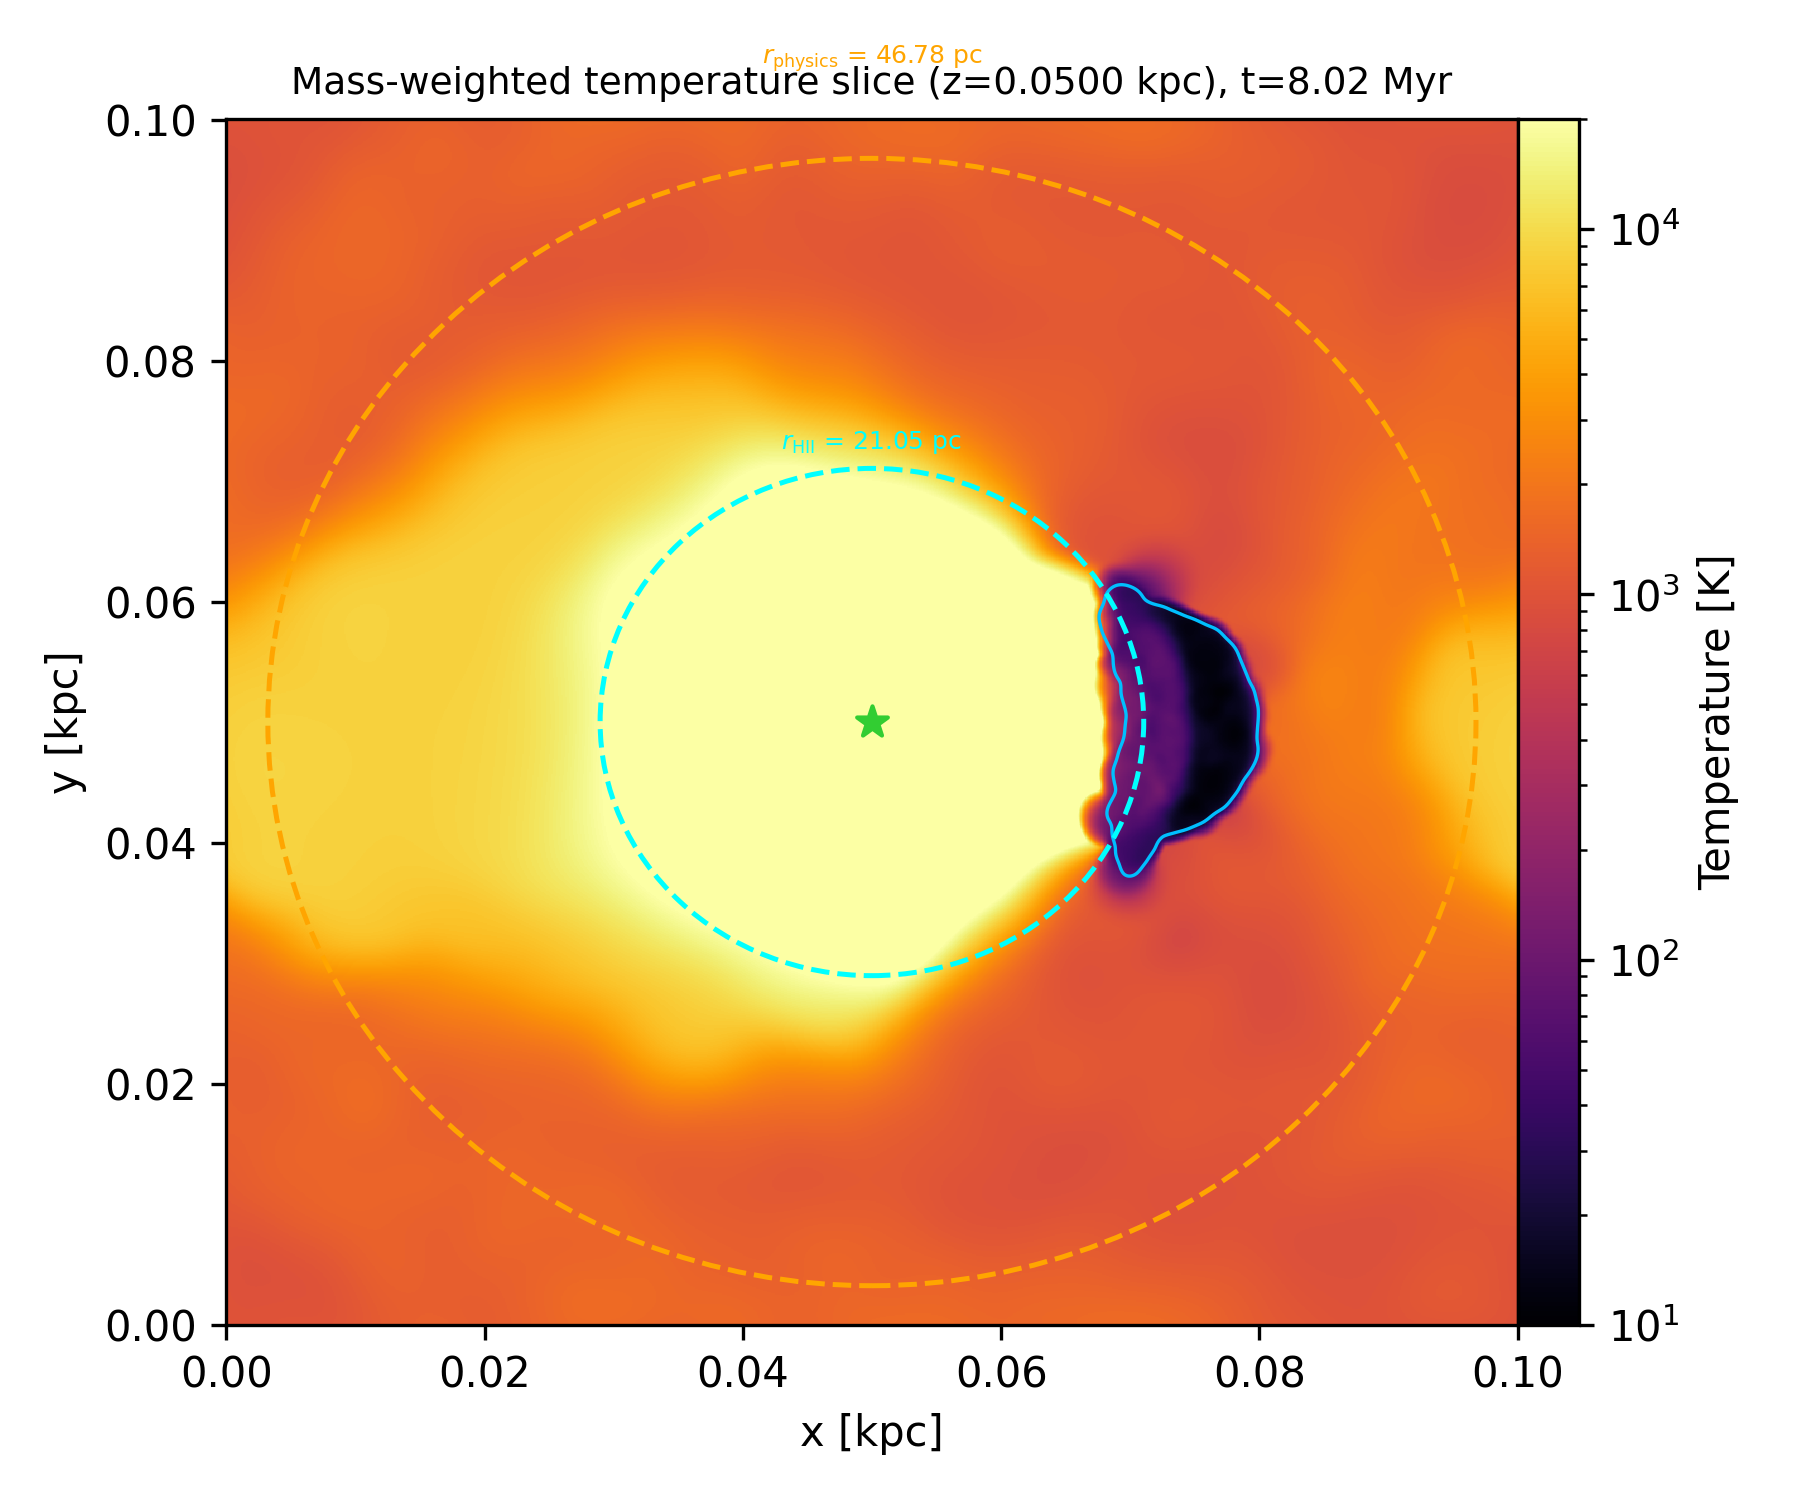
\includegraphics[width=0.325\linewidth]{Figures/tslice_gas95z0_nside0_rebuild0p01} &
    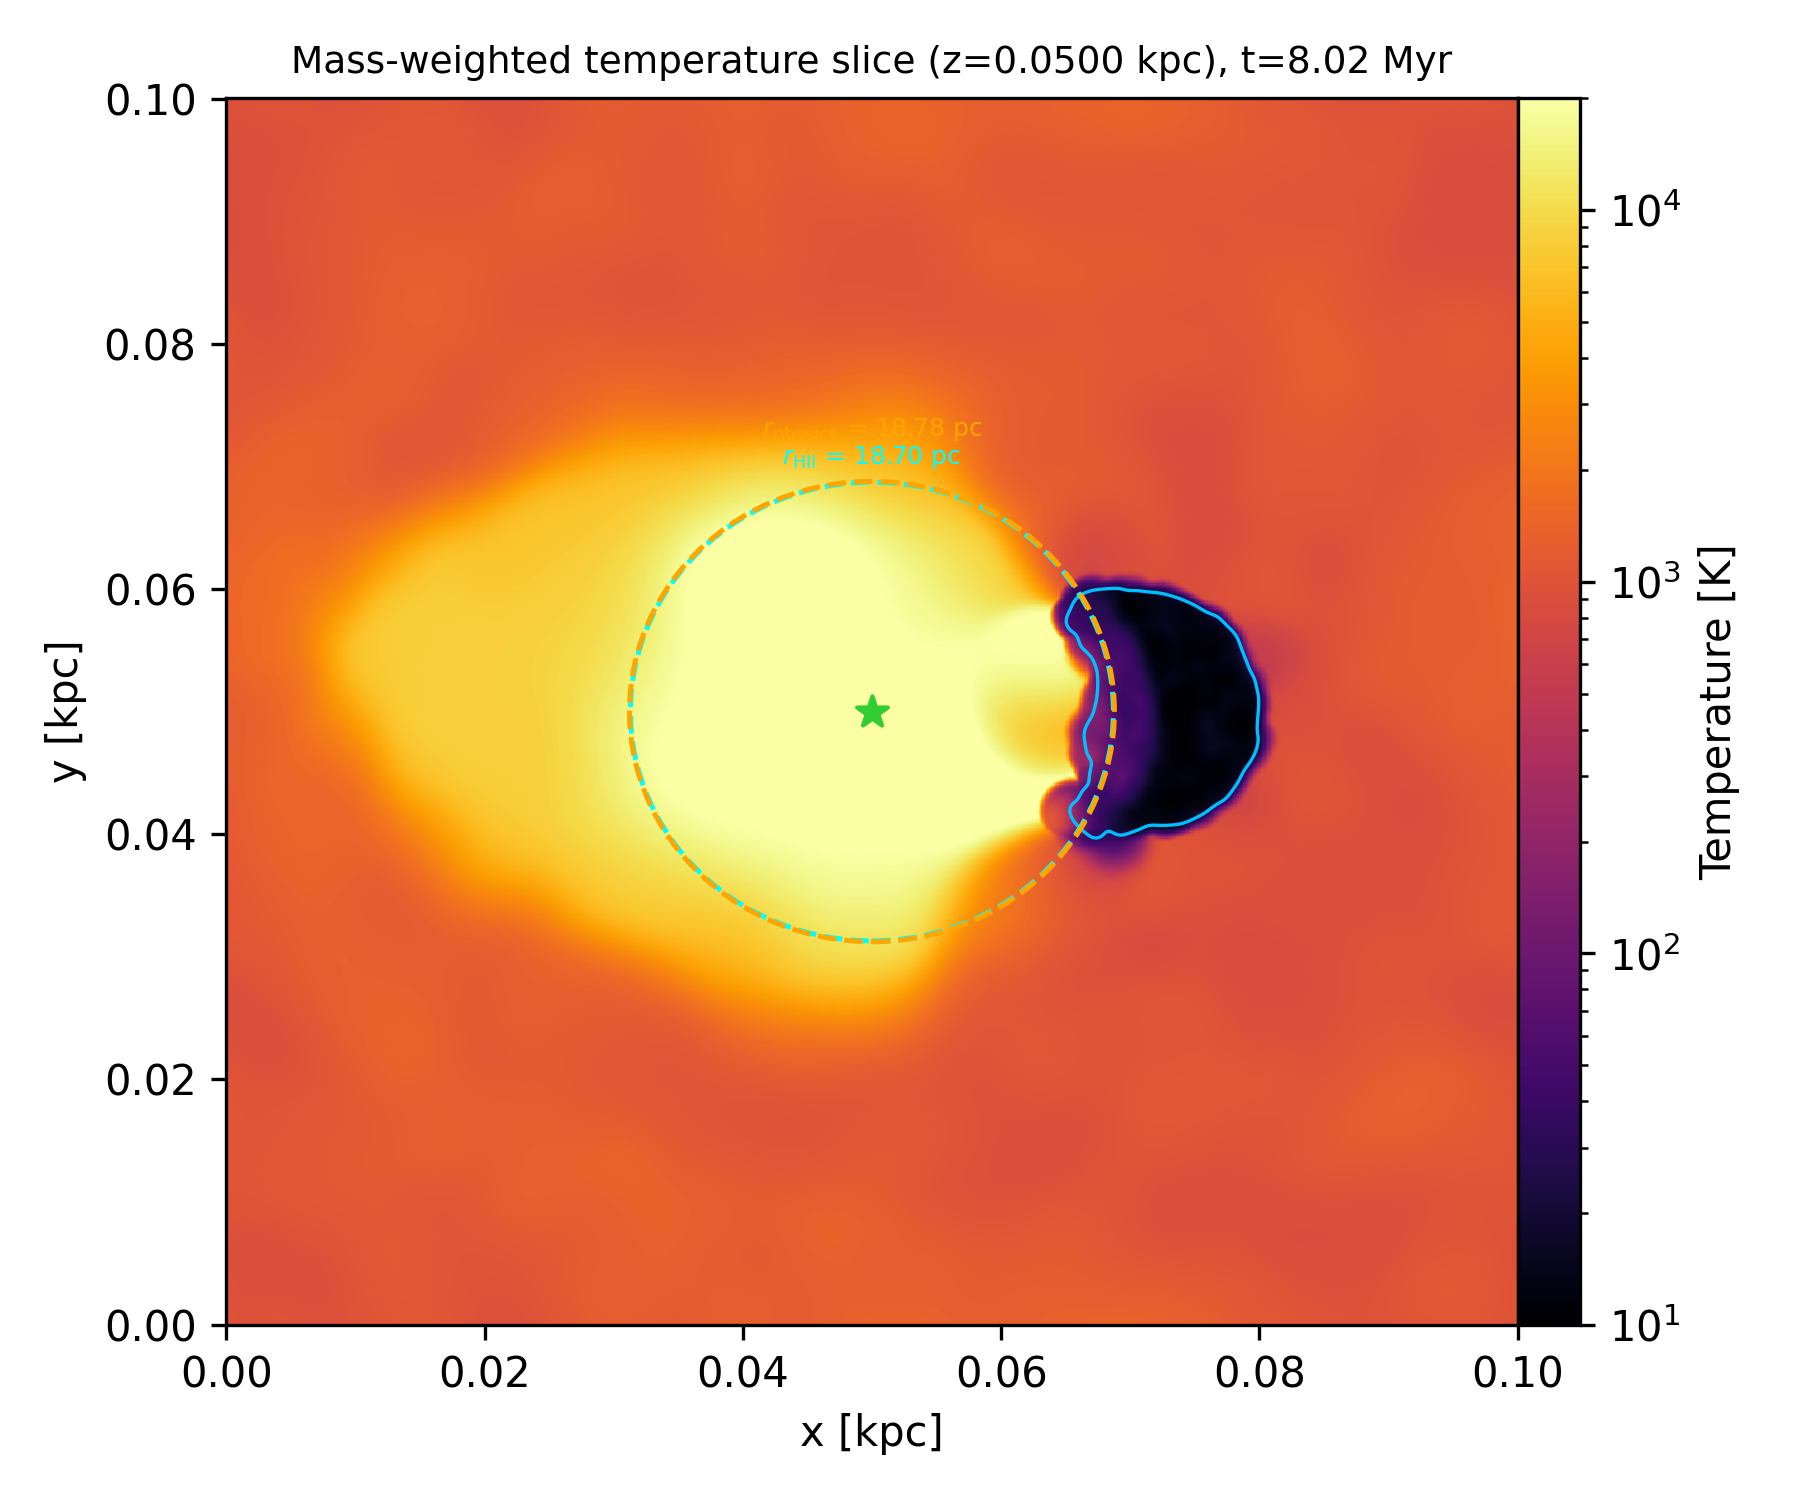
\includegraphics[width=0.325\linewidth]{Figures/tslice_gas95z0_nside0_rebuild0p05} &
    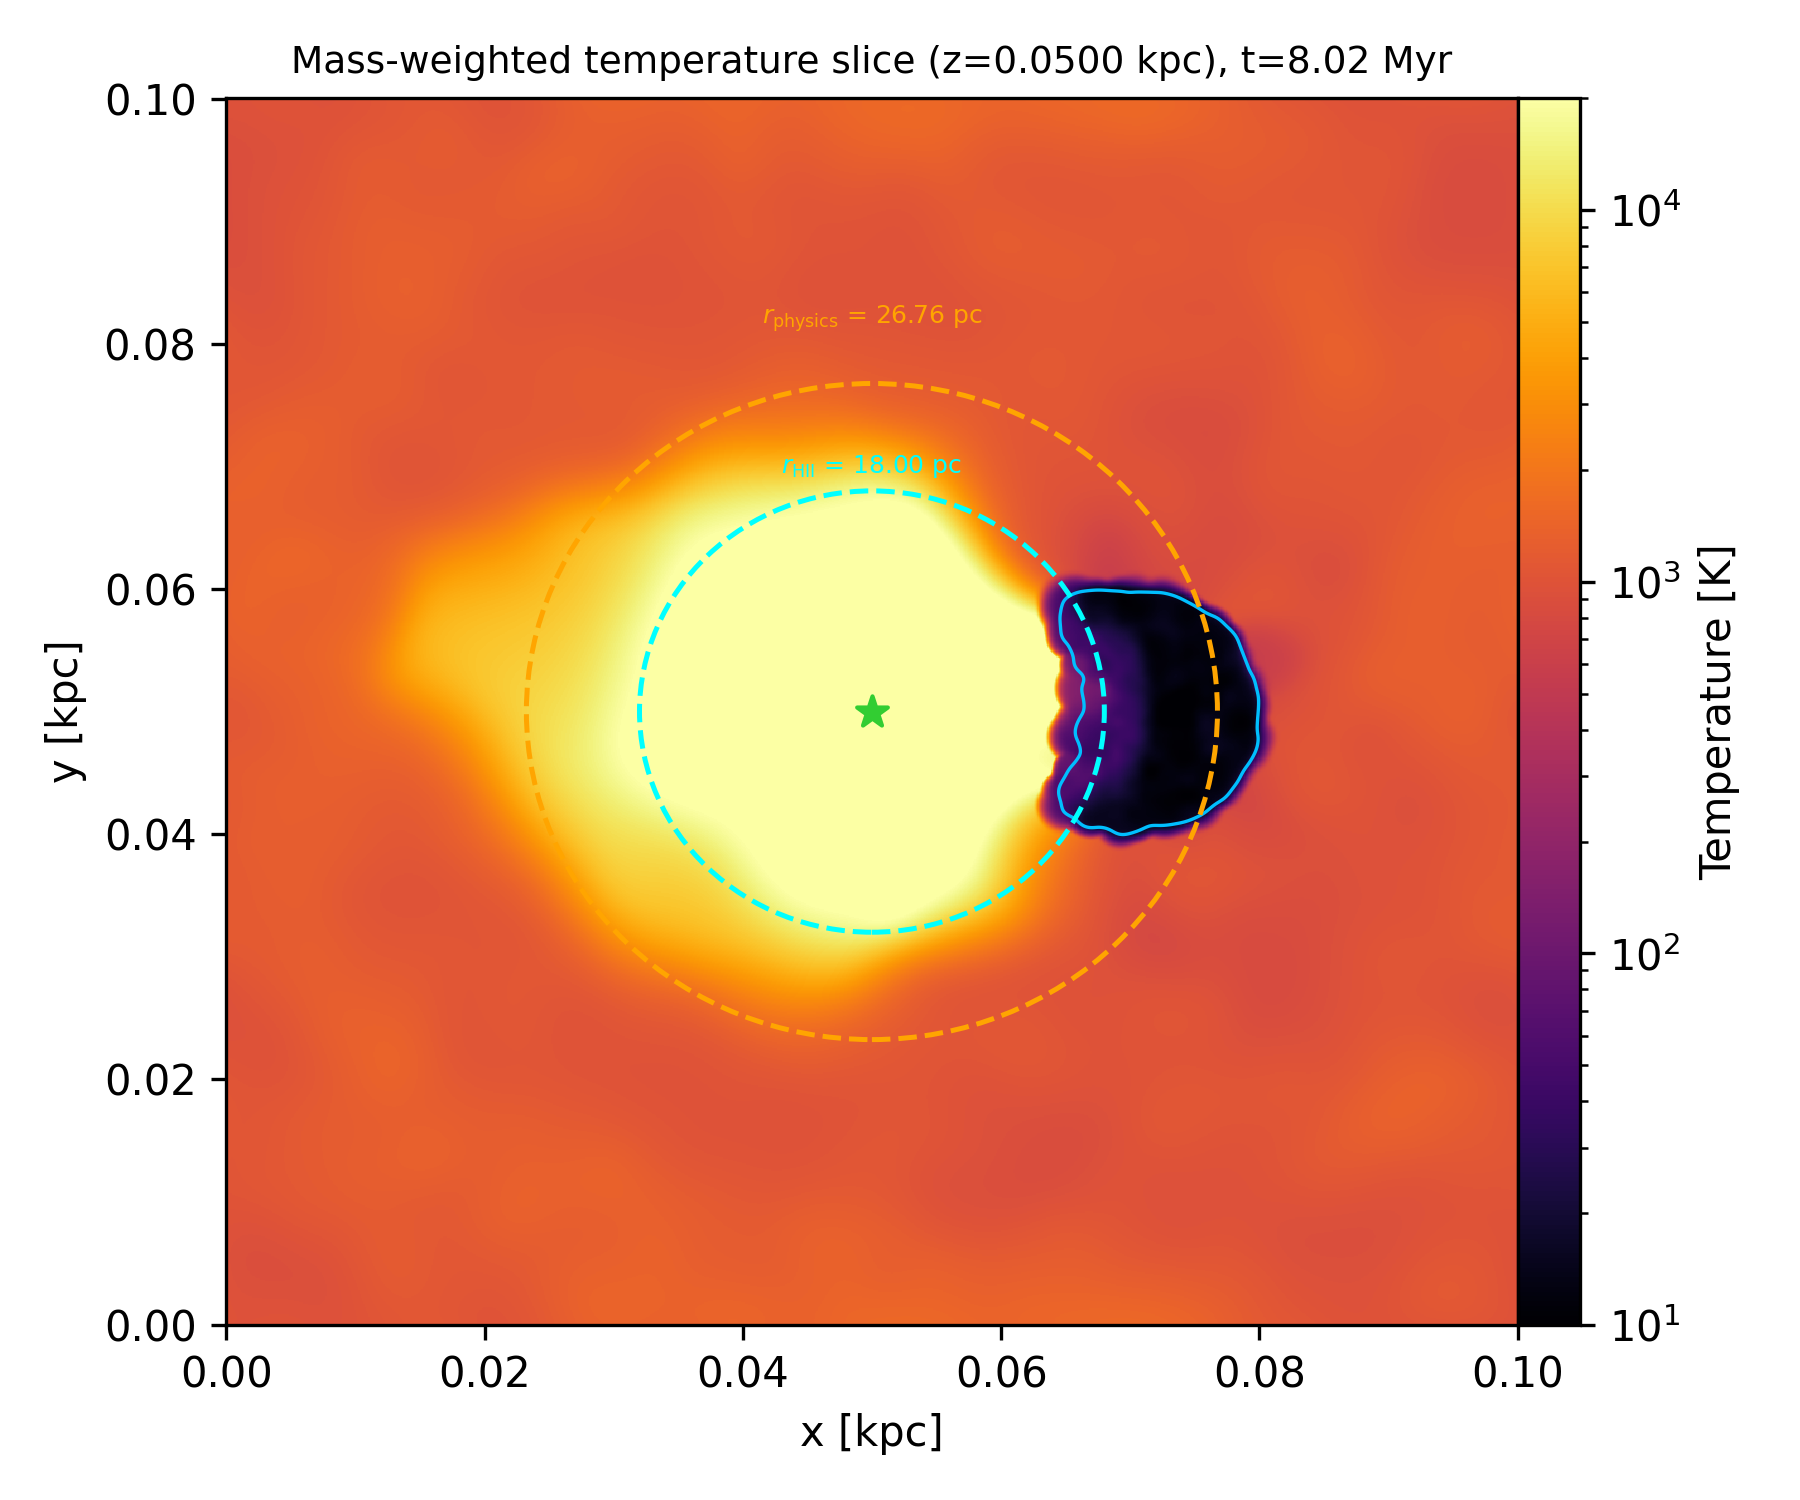
\includegraphics[width=0.325\linewidth]{Figures/tslice_gas95z0_nside0_rebuild0p1} \\
    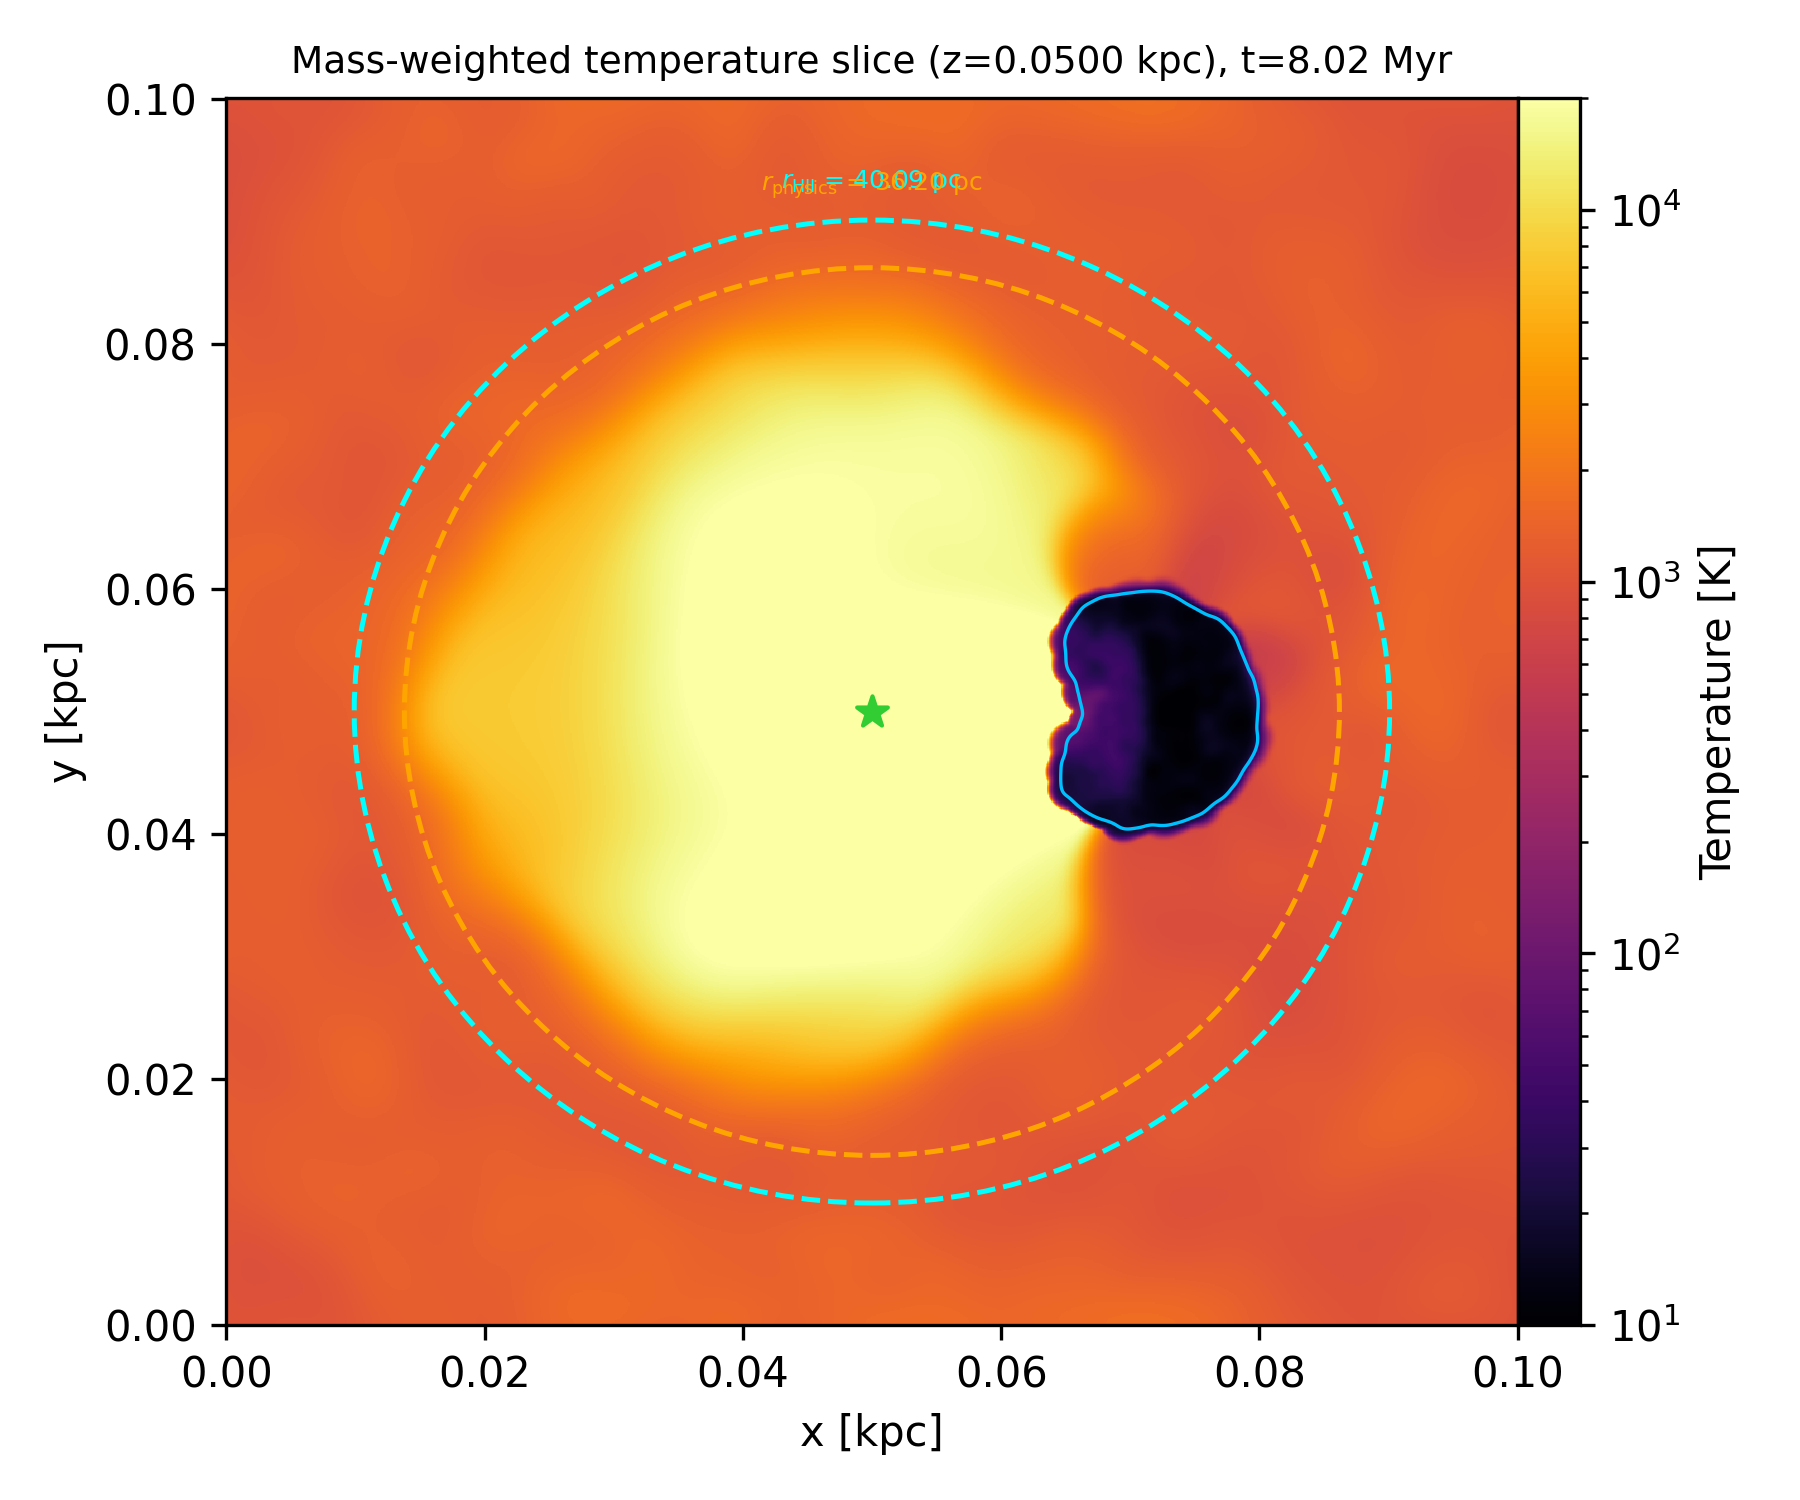
\includegraphics[width=0.325\linewidth]{Figures/tslice_gas95z0_nside1_rebuild0p01} &
    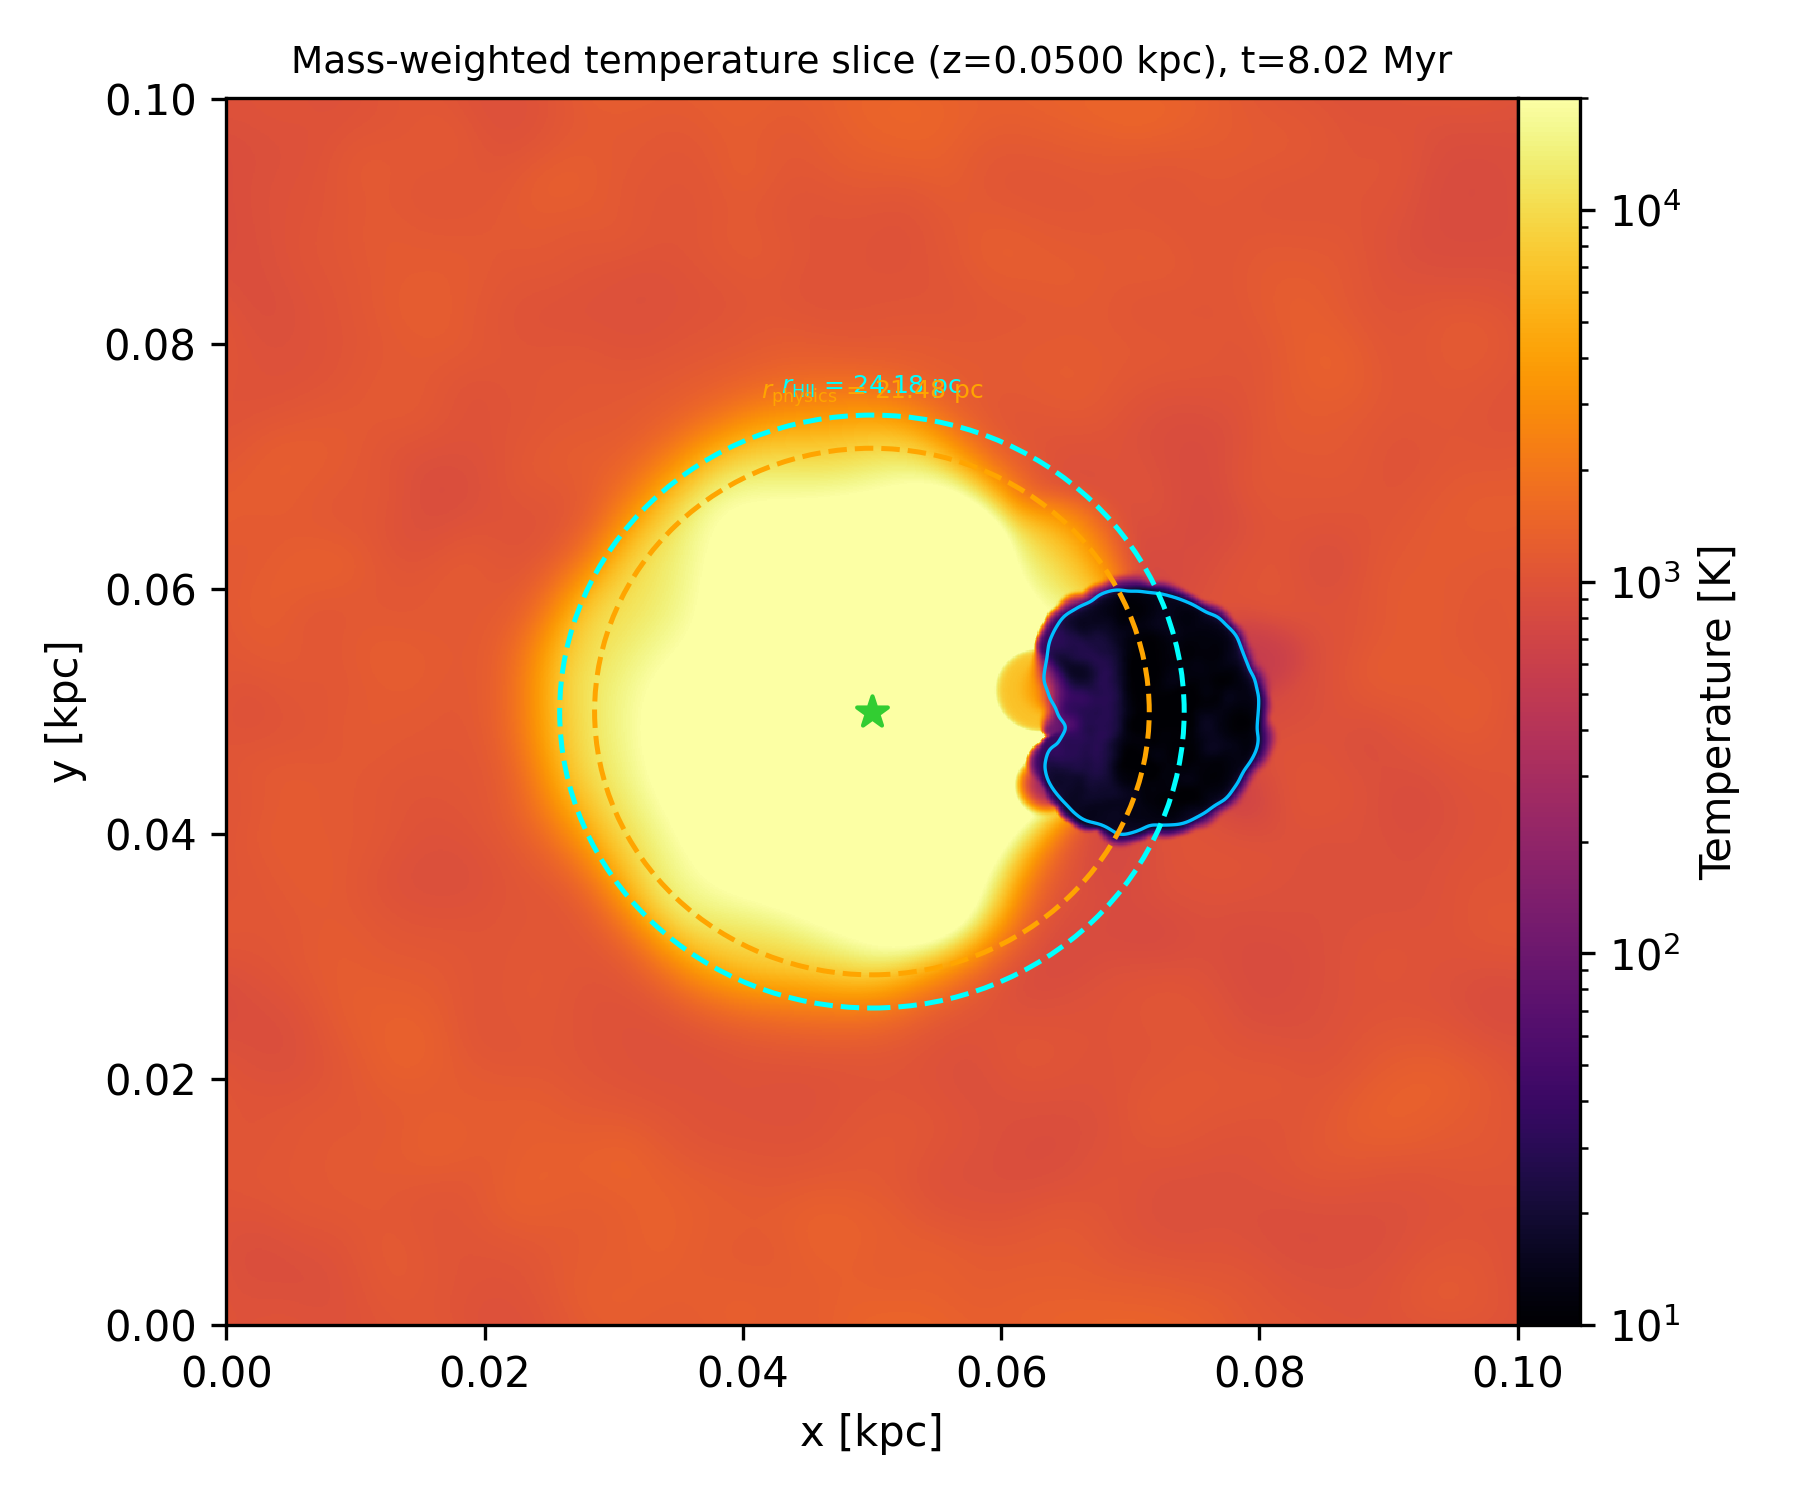
\includegraphics[width=0.325\linewidth]{Figures/tslice_gas95z0_nside1_rebuild0p05} &
    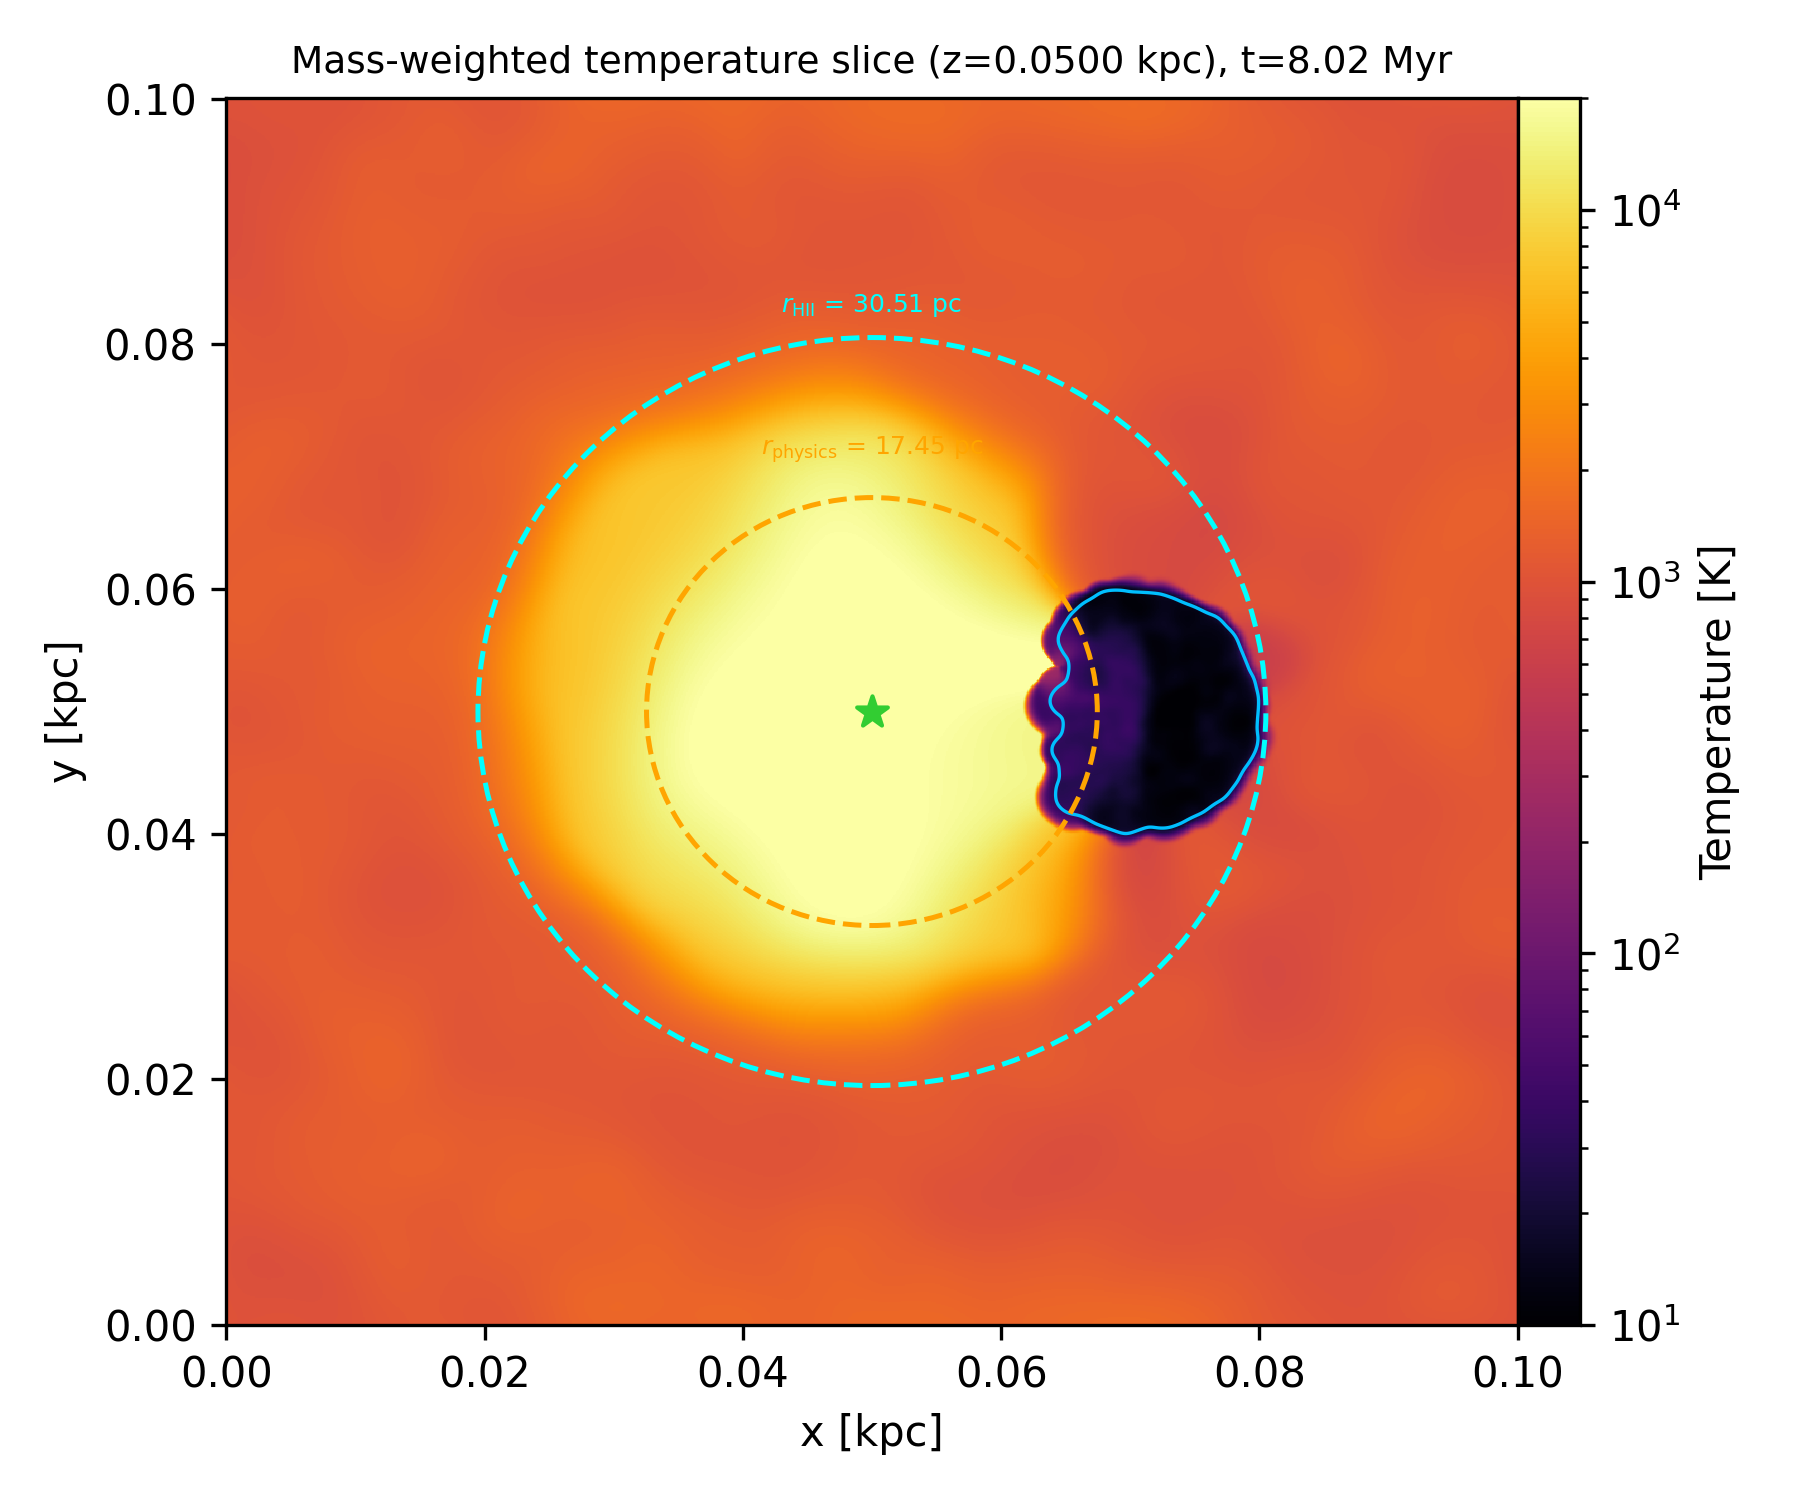
\includegraphics[width=0.325\linewidth]{Figures/tslice_gas95z0_nside1_rebuild0p1} \\
  \end{tabular}
  \caption{Temperature slices at $t=8\,$Myr, \texttt{gas\_mass=95},
    $Z=0$. Same layout and markers as
    Figure~\ref{fig:gas20-z0-slices}. Compare against
    Figure~\ref{fig:gas95-slices}.}
  \label{fig:gas95-z0-slices}
\end{figure}

\textbf{On the ``angular vs.\ uniform difference is not pronounced''
concern:} it is more pronounced at $Z=0$ in absolute terms --
Figure~\ref{fig:gas20-z0-growth} shows angular reaching 42--45\,pc
against uniform's $\approx$16--21\,pc (a factor of $\sim$2--2.5,
versus the $\sim$1.7$\times$ spread at
$Z/Z_\odot\approx0.231$, Figure~\ref{fig:gas20-growth}) -- but the
warm-background contamination described above means this spread is not
as visually clean in the temperature-slice panels
(Figure~\ref{fig:gas20-z0-slices}) as it is at
$Z/Z_\odot\approx0.231$ (Figure~\ref{fig:gas20-slices}), where the
clump notch and bubble edge stand out sharply against black. Both
effects raised above -- the lower $\beta(T)$ inflating both curves,
and cooling contamination blurring the visual contrast -- point the
same way: \textbf{$Z/Z_\odot\approx0.231$ remains the more diagnostic
configuration for judging the angular scheme's clump-erosion behaviour
by eye; the $Z=0$ matrix here is this example's actual default
behaviour, not a cleaner comparison.}

\subsection{D-type growth curve shape (e10)}
\label{sec:e10}

The matrix above compares only final-time values. \citet{Spitzer1978}'s
classical D-type expansion solution gives the full trajectory, not just
the endpoint:
\begin{equation}
  R(t) = R_{\rm st}\left(1 + \frac{7 c_s t}{4 R_{\rm st}}\right)^{4/7},
  \label{eq:dtype}
\end{equation}
where $R_{\rm st}$ is the equilibrium Str\"omgren radius and $c_s$ is
the isothermal sound speed of the ionized gas. \code{stromgren\_\allowbreak
analytic\_check.py} (sibling \code{StromgrenSphere} example)
reimplements this directly from the code's own $\dot N_{\rm ion}(m)$
fit (not an independently-guessed photon budget), using this run's
actual applied ionized temperature for both $\alpha_B$ and $c_s$
(Section~\ref{sec:metallicity}) rather than the classical $10^4\,$K
reference point, since using the latter would systematically
under-predict the analytic curve for any $Z=0$ run and make a real
match look like a mismatch.

A single-star run (no clump, no co-location, matching e10's
requirement) needed a box wide enough to contain the equilibrium
radius and a long enough \code{time\_end} to see the curve plateau
without extending past the star's own ionizing lifetime -- the
example's own defaults (25\,pc box half-width, $R_{\rm st}=26.4\,$pc
for the default $29.7\,{\rm M}_\odot$ star) do not satisfy the first
condition, so this run uses \code{boxsize=0.08} (80\,pc) and
\code{time\_end=1.2e-2} ($\approx$11.7\,Myr) instead, via new
\code{run.sh} overrides added for this check.

\todo{Run in progress at time of writing
(\code{run\_name=e10\_fixed\_box\_and\_time}). Fill in the
simulated-vs-analytic comparison, pass/fail, and a plot once it
completes.}
